\documentclass[twoside,11pt]{starlink}

% ? Specify used packages
% ? End of specify used packages

% -----------------------------------------------------------------------------
% ? Document identification
\stardoccategory    {Starlink User Note}
\stardocinitials    {SUN}
\stardocsource      {sun\stardocnumber}
\stardocnumber      {223.7}
\stardocauthors     {D.S. Berry \& T.M. Gledhill }
\stardocdate        {17th December 2012}
\stardoctitle       {POLPACK \\
                            An Imaging Polarimetry Reduction Package}
\stardocversion     {Version 3.2-0}
\stardocmanual      {Users' Manual}
\startitlepic {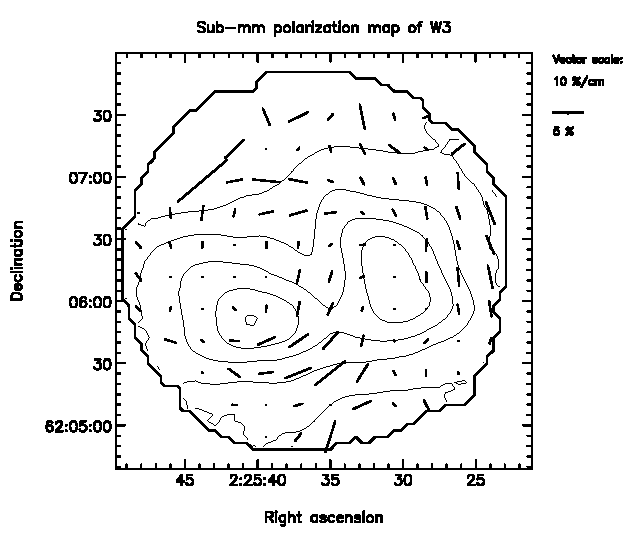
\includegraphics[clip,scale=1.0]{sun223_figures/fig}}
\stardocabstract  {POLPACK is a package of applications for
reducing imaging polarimetry or spectropolarimetry data. They cover
registration, sky subtraction, calculation of Stokes parameters, and
display of vector maps.

\emph{The polarization map on the front cover shows 850 $\mu$m dust grain
emission in the cloud core W3. The map shows large scale magnetic fields
in this region of high-mass star-formation. The data were obtained with
the SCUBA polarimeter on the James Clerk Maxwell Telescope  (operated by
the Joint Astronomy Centre in Hawaii), and reduced using SURF and POLPACK.
}
}

% ? End of document identification
% -----------------------------------------------------------------------------
% -----------------------------------------------------------------------------
% ? Document specific \providecommand or \newenvironment commands.

% centre an asterisk
\providecommand{\lsk}{\raisebox{-0.4ex}{\rm *}}

% Environment for indenting and using a small font.
\newenvironment{myquote}{\begin{quote}\begin{small}}{\end{small}\end{quote}}

% In-line typed text, buttons and menu items.
\providecommand{\butt}[1]{{\small \bf \tt #1}}
\providecommand{\menu}[1]{{\small \bf \em #1}}
\providecommand{\wlab}[1]{{\small \bf #1}}
\providecommand{\text}[1]{{\small \tt #1}}

% Quick routine descriptions
\providecommand{\quickdes}[3]{
                         \parbox{1.1in}{\textbf{#1}}
                         \parbox{4.4in}{\raggedright #2 \dotfill}
                         \parbox{0.6in}{\pageref{#3}}
                         \vspace*{0.2in}}

% Quotes for SST.
\providecommand{\qt}[1]{\texttt{"}#1\texttt{"}}
\providecommand{\qs}[1]{\texttt{'}#1\texttt{'}}



% Routines with descriptions in the appendix.
\providecommand{\routine}[1]{\textsc{#1}}
\providecommand{\xroutine}[1]{\htmlref{\textsc{#1}}{#1}}

% degrees symbol
\providecommand{\dgs}{\hbox{$^\circ$}}

\providecommand{\dash}{--}


\providecommand{\STARURL}{http://www.starlink.ac.uk}
\providecommand{\TCLURL}{http://www.scriptics.com/}
\providecommand{\IRAFURL}{http://www.starlink.ac.uk/iraf/web/iraf-homepage.html}
\providecommand{\STORE}{http://www.starlink.ac.uk/cgi-bin/storetop}

\providecommand{\latexonlysection}[1]{\section{#1}}

% ? End of document specific commands
% -----------------------------------------------------------------------------
%  Title Page.
%  ===========
\begin{document}
\scfrontmatter

\section{\xlabel{introduction}Introduction}
POLPACK is a package of applications for mapping the linear or circular
polarization of extended astronomical objects, either in a single
waveband, or in multiple wavebands (spectropolarimetry). Data from both
single and dual beam polarimeters can be processed\footnote{At the
moment, circular polarization can only be measured when using dual-beam
data.}.

POLPACK processes data in \emph{NDF} format. This is the standard data
format used by most Starlink software, and is described fully in
\xref{SUN/33}{sun33}{}. However, other astronomical data formats may also
be processed using transparent on-the-fly data conversion facilities
provided by the NDF subroutine library, and the CONVERT package. The use of
these facilities is described \slhyperref{here}{in section }{}{SEC:CONVERT},
and more fully in \xref{SUN/55}{sun55}{}.

The facilities provided by POLPACK include:
\begin{itemize}
\item alignment of images on the sky.
\item extraction of $O$ and $E$ images from individual frames of dual-beam
data.
\item sky subtraction.
\item calculation of Stokes parameters.
\item binning of Stokes parameters.
\item creation of catalogues of polarization vectors.
\item graphical display of vector maps.
\end{itemize}

POLPACK does not provide facilities for performing instrumental
corrections such as flat-fielding, de-biassing, \emph{etc}. Such corrections
should be applied to the data before using POLPACK, so that POLPACK can
assume that pixel values are proportional to the combined intensity of
sky and object. Further comments on these corrections can be found
\slhyperref{here}{in section }{}{SEC:CCDPACK}.

Slightly different facilities are available when using single-beam or
dual-beam data, as described in the following sections\footnote{It is
hoped to rationalize the differences between these two modes in future
releases.}.

\subsection{Single-beam Facilities}

\begin{itemize}

\item Data from polarimeters or spectropolarimeters containing the following
optical components can be processed:

\begin{enumerate}
\item A fixed analyser and a rotating half-wave plate.
\item Multiple fixed analysers.
\item A single rotating analyser.
\end{enumerate}

\item Only linear polarization can be measured.

\item Different target exposures can be rotated with respect to one
another. That is, the linear mapping between corresponding positions in
any two target
exposures can include rotation, as well as magnification and a shift of
origin (shear is not allowed).

\item The transmission and efficiency of non-perfect analysers can be
taken into account, if known values for these quantities are available.

\item Estimates of the variance in the observed intensity images can be made
if necessary. This is useful if your data does not have usable variance
information associated with it. Variances on the reduced quantities
(Stokes vectors, polarization vectors, \emph{etc.}) can then be calculated
on the basis of these estimated input variances.

\item The observed intensity images must all have the same normalization.
That is, the ``exposure times'' are all assumed to be equal.

\end{itemize}

\subsection{Dual-beam Facilities}

\begin{itemize}

\item It is assumed that the polarimeter or spectropolarimeter contains a
fixed analyser and a rotating half or quarter wave-plate which is stepped
in units of 45\dgs.

\item Both linear and circular polarization can be measured.

\item Different target exposures must not be rotated with respect to one
another. That is, the linear mapping between corresponding positions in any two target
exposures can only include magnification and a shift of origin (rotation
and shear are not allowed).

\item The analyser is assumed to be perfect (\emph{i.e.} the transmission and
efficiency of the analyser are both assumed to be $1.0$).

\item Variances can only be calculated for the reduced quantities (Stokes
vectors, polarization vectors, \emph{etc.}) if the observed intensity
images have usable variances associates with them (\emph{i.e.} these
input variances cannot be estimated for dual-beam data).

\item Corrections can be applied when calculating the Stokes vectors which
take account of any differences in the exposure times between raw frames,
and any difference in the sensitivity of the two channels of the
dual-beam polarimeter. They rely on redundancy in the supplied data, and
require a specific set of analyser positions to be used (described
\slhyperref{here}{in section }{} {SEC:DETCOR}) when obtaining the data.

\end{itemize}

\section{\label{SEC:DBPOL}\xlabel{dualbeampolarimetry}Dual-beam Polarimetry}
This section gives a brief introduction to the general principles of
dual-beam polarimetry. It explains words and concepts used later, and
defines the data model used by POLPACK. A well established example of a
dual-beam polarimeter is described by Scarrott et al. (\emph{Mon. Not. R.
astr. Soc.} (1983) \textbf{204}, 1163 - 1177).

Single waveband polarimetry is described here but the principles can be
extended to imaging spectropolarimetry (see \slhyperref{here}{section }{}{SEC:SPEC}).

\subsection{The Polarimeter}
A dual-beam polarimeter suitable for measuring linear polarization usually
contains the following optical components:

\begin{enumerate}
\item A focal-plane \emph{mask}.
\item A \emph{half-wave plate}.
\item An \emph{analyser}.
\item A \emph{detector}.
\end{enumerate}

The light collected by the telescope passes through these components in
the order listed (see Figure~\ref{fig:optical}).
Each component is described more fully below.

  \begin{figure}[htb]
  \begin{center}
  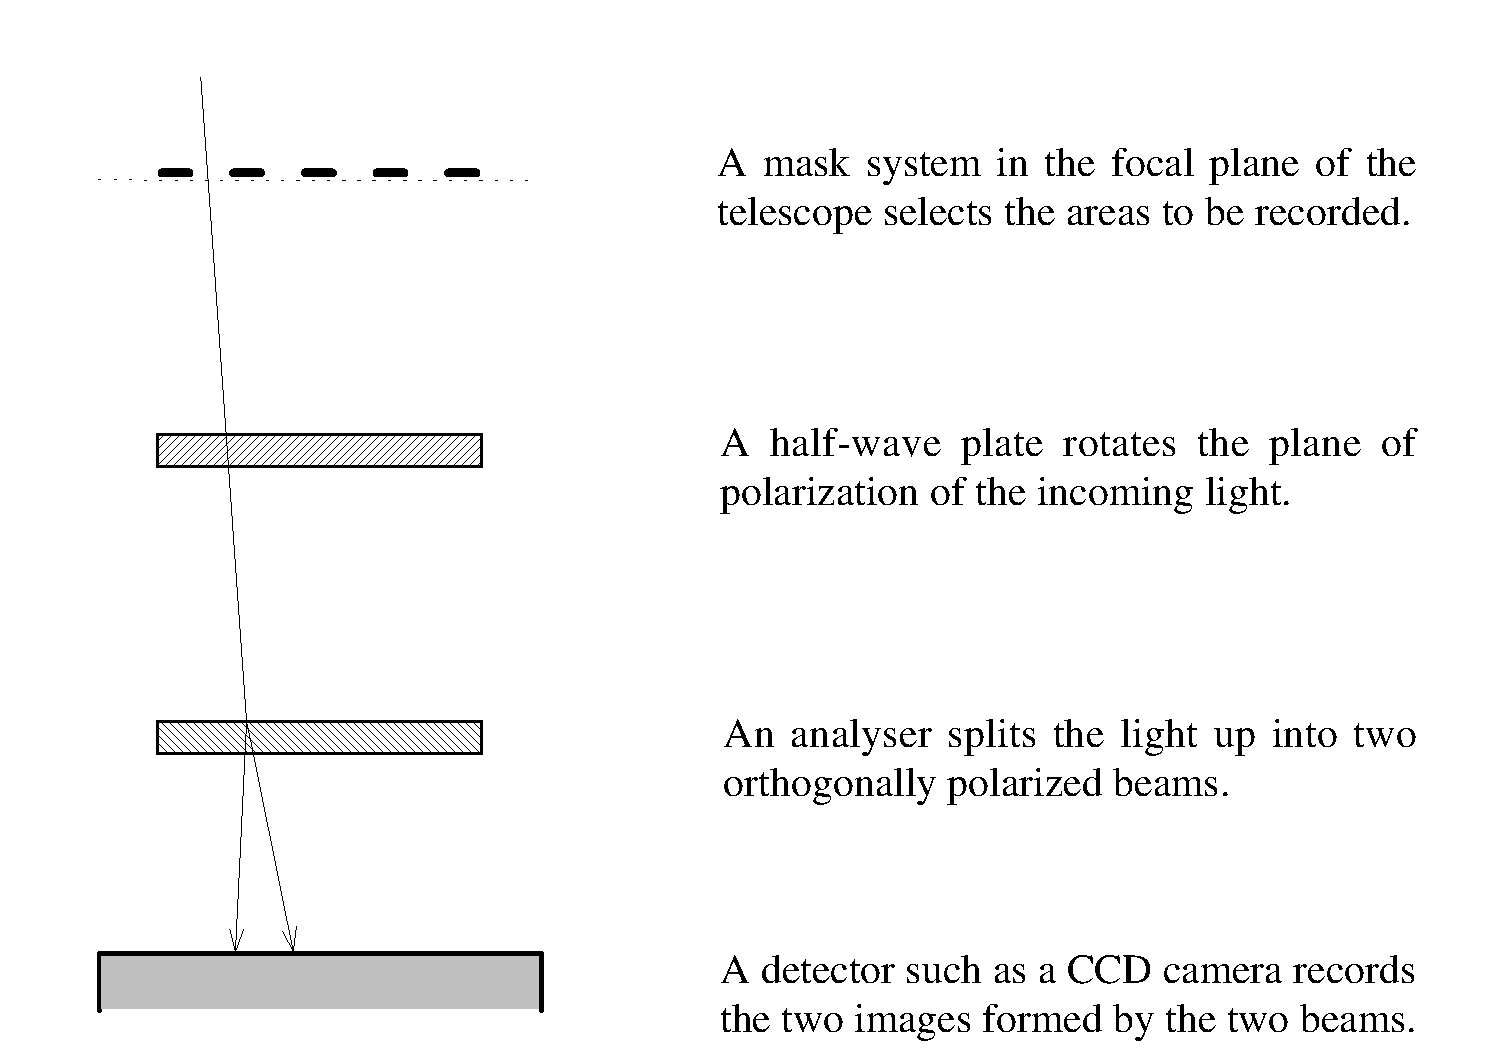
\includegraphics[clip,scale=0.5]{sun223_figures/optical}
  \caption{The main optical components in a typical dual-beam imaging polarimeter.}
  \label{fig:optical}
  \end{center}
  \end{figure}

The heart of the polarimeter is the \emph{analyser}, which splits incoming
partially plane polarized light up into two beams; one (called the
ordinary, or $O$ ray) contains the component of the incoming light
which is polarized parallel to the axis of the analyser, and the other
(called the extraordinary, or $E$ ray) contains the component of the
incoming light which is polarized orthogonally to the axis of the
analyser. These two beams are recorded simultaneously on a suitable
detector such as a CCD. The advantage of this system over a single-beam
instrument (in which only one state of polarization is recorded on a
given exposure), is that variations in sky background between exposures
affect both states of polarization equally, and so can be eliminated.

In an imaging polarimeter, the two beams form two images on the detector,
displaced by some distance determined by the design of the instrument;
both images representing the same area of the sky. A \emph{masking system}
is used to prevent any overlap between the two images. In some
instruments this takes the form of a series of parallel, equally spaced
bars in the focal plane of the telescope (see
Figure~\ref{fig:grids}). In
this case, the instrument is designed so that the displacement between
the two images formed by the $O$ and $E$ rays is perpendicular to the
bars, and equal in size to the width of a bar. Thus, the two images form
two inter-leaving sets of bars. There are several other systems (such as
a mask containing only a single aperture), but the principle is the same.

  \begin{figure}[p]
  \begin{center}
  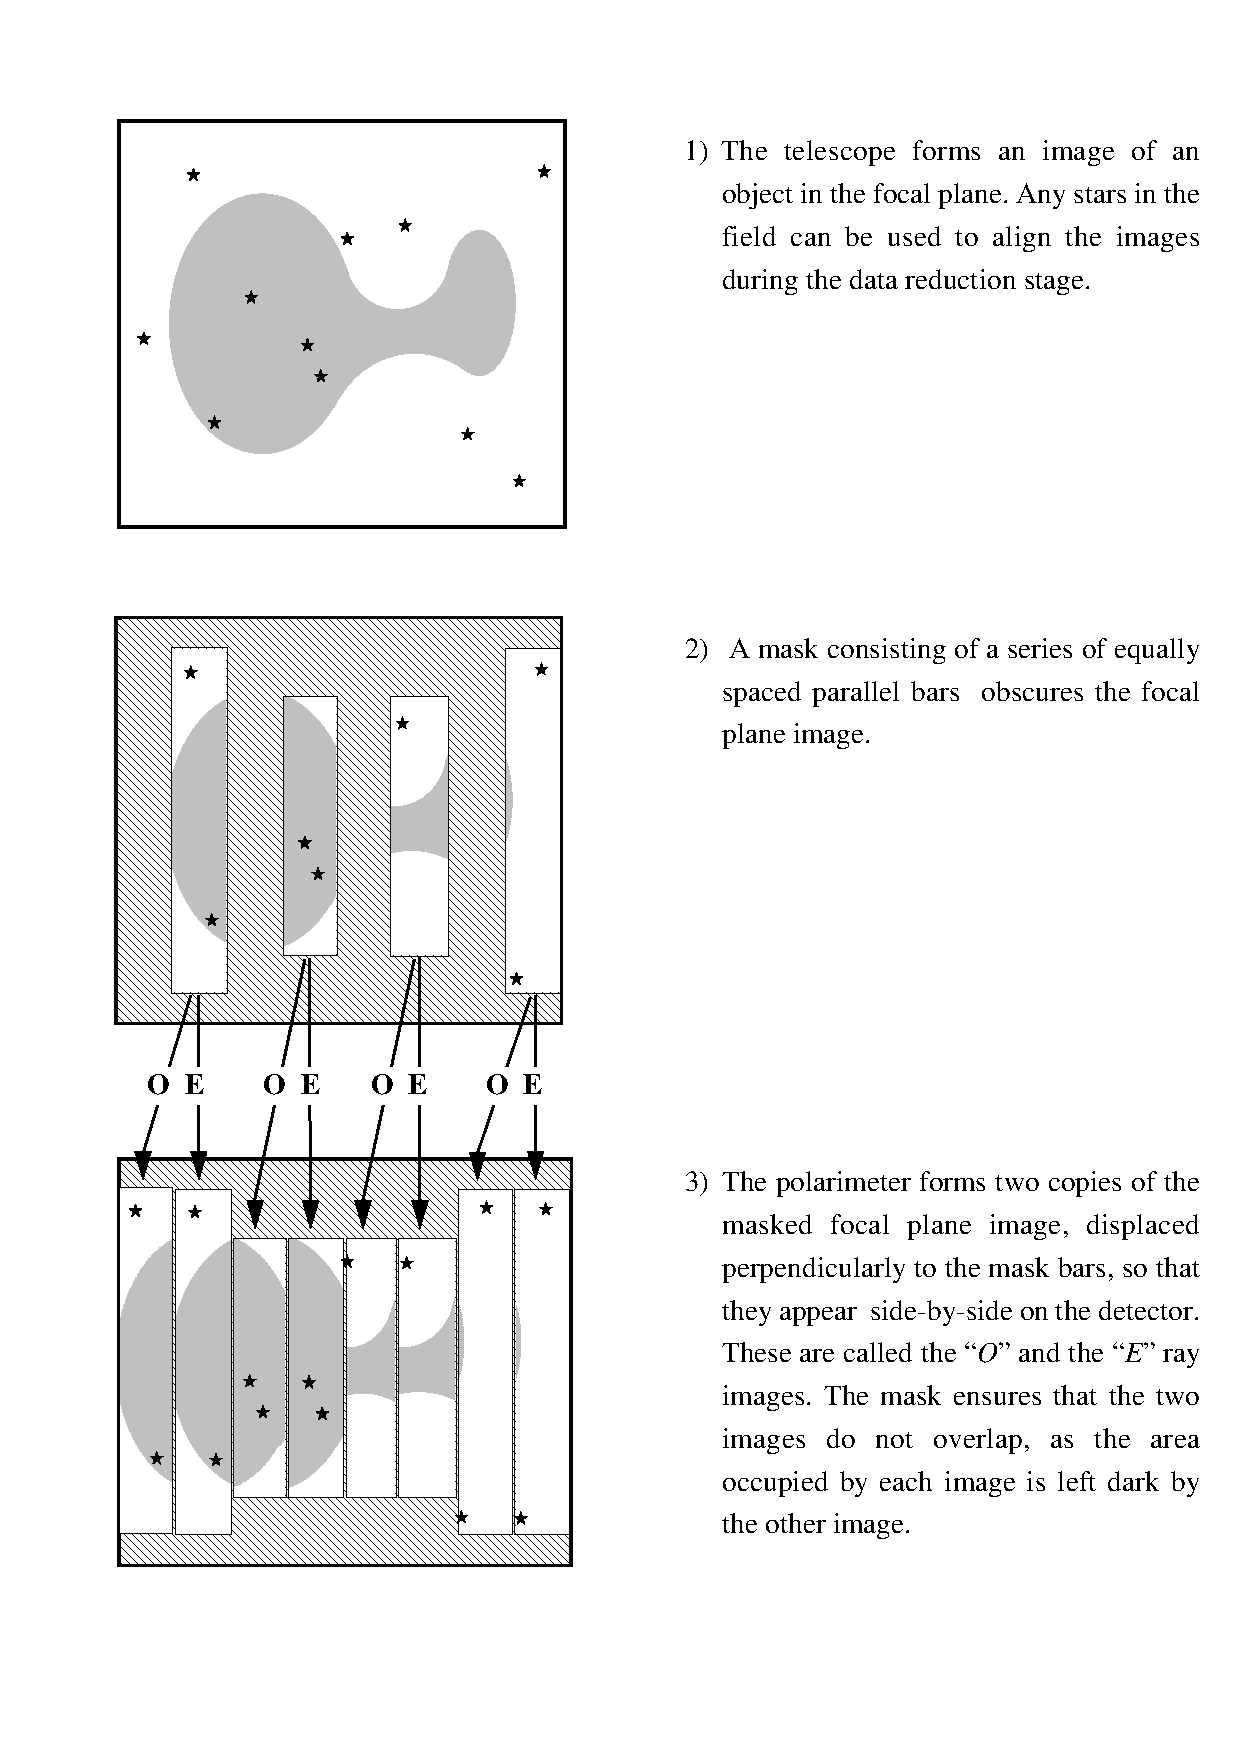
\includegraphics[clip,scale=0.8]{sun223_figures/grids}
  \caption{An example of a masking system used in a dual-beam imaging polarimeter.}
  \label{fig:grids}
  \end{center}
  \end{figure}

If the incoming light is only partially polarized, then at least two
exposures are required to estimate both the degree and the orientation of
the polarization, each exposure recording the intensity in two orthogonal
states of polarization as described above. The analyser axis is rotated
in steps of 45\dgs\ between these exposures. In practice, physically rotating
the analyser would result in the displacement between the $O$ and
the $E$ ray images also rotating. This would cause the images to overlap
on the detector and would make the data reduction process much harder (if
not impossible). For this reason, the analyser is usually left in a fixed
position, and the plane of polarization of the incoming light is rotated
instead. This is achieved by placing a \emph{half-wave plate} in
front of the analyser, and rotating it in steps of 22.5\dgs, resulting in
a rotation of the plane of polarization of 45\dgs. Using this scheme the
positions of the $O$ and $E$ ray images on the detector are unchanged.

The orientation of the plane of polarization of the incoming light is
measured relative to a fixed ``reference'' direction. The analyser axis
and the 0\dgs\ position of the half-wave plate are usually parallel to
this direction.

\subsection{\label{SEC:OBS}\xlabel{theobservationalprocedure}The Observational Procedure}
At least two exposures are required to estimate the degree and
orientation of the polarization, taken with half-wave plate positions of
0\dgs\ and 22.5\dgs\ (see \slhyperref{here}{appendix }{}{APP:POL}). For ease
of reference, these exposures are referred to here as $T_{0}$ and
$T_{22.5}$. The $O$ and $E$ ray images in $T_{0}$ measure the intensities
parallel and perpendicular to the reference direction. $T_{22.5}$ has an
effective analyser angle of 45\dgs\ (twice the half-wave plate angle) and
so measures the intensities at angles of 45\dgs\ and 135\dgs\ to the
reference direction

Usually, a further two exposures are taken at half-wave plate positions
of 45\dgs\ and 67.5\dgs\ (referred to here as exposures $T_{45}$ and
$T_{67.5}$). These provide some redundancy in the data and enable
internal consistency checks to be made during the data reduction stage.

These exposures are denoted by the letter $T$ to indicate that they are
\emph{target} exposures. In addition to these target exposures, some \emph{flat-field} exposures are also required. These are used to correct for
any spatial variation in the sensitivity of the system, and consist of
exposures of a photometrically flat surface. Ideally, the flat-field
source should be unpolarized. However, if the additional target exposures
$T_{45}$ and $T_{67.5}$ are taken, then a spatially constant polarization
across the flat-field source can be corrected for during data reduction.
Since the polarization of the flat-field surface is rarely known to be
zero, these additional target exposures should always be taken.

It is important that the flat-field has a good signal-to-noise ratio.
For this reason, it is common practice to take one or more flat-field
exposures at each half-wave plate position, and stack them together into a
single master flat-field (although it is not strictly necessary to use
different half-wave plate positions). Further discussion of the flat-fielding
procedure is given \slhyperref{here}{in section }{}{SEC:DETCOR}.

\subsection{\label{SEC:DBRED}\xlabel{thedatareduction}The Data Reduction}
Several steps are involved in the production of a polarization map from
the raw exposures recorded by the detector. An over-view of these steps
is given here. Details of how they may be implemented in practice using
POLPACK are given in later sections of this document.

\subsubsection{\label{SEC:DETCOR}Corrections Related to the Detector}
These convert the raw data numbers measured by the detector into values
which are proportional to the combined sky and object intensity
transmitted by the analyser (plus noise of course). The details of these
corrections will depend on the nature of the detector. For a CCD camera,
they will usually involve at least flat-fielding, and de-biassing.

Flat-fielding is worthy of some extra discussion, since it can be
complicated by the presence of the polarimeter in the light path. The
purpose of flat-fielding is to ensure that there are no spatial
variations in the sensitivity of the detector. This is normally achieved
by taking images of a photometrically flat surface such as the inside of
the observatory dome, or the twilight sky\footnote{In the near infra-red
flat-fields are normally taken on the night sky which at these wavelengths
is bright enough to give a good signal to noise ratio.}. Since the
brightness of this surface is constant, any variations in the recorded
image (the ``flat-field'' image) must be due to variations in the
sensitivity of the detector. These variations can then be removed from the
target observation by dividing every pixel value in the target image by
the corresponding pixel value in the flat-field image.

Introducing a polarimeter into the light path can complicate this if the
flat-field is taken in polarized light (such as is produced by reflective
surfaces in the dome, or by light scattering in the atmosphere). In this
case the intensity of the light reaching the detector will not be
constant across the field, but will depend on the polarization.

If the polarization of the flat-field is non-zero and spatially constant,
then the $O$ and $E$ ray flat-field images will have different mean
values (visible as sharply defined dark and light areas in the flat
field). If such a flat-field is used to correct the target exposures,
then the different mean values in the flat-field will result in an
apparent difference in sensitivity between the two channels of the
polarimeter (known as the ``F-factor''). Such a difference in sensitivity
can be corrected for when calculating the polarization if the additional
target exposures \slhyperref{$T_{45}$ and $T_{67.5}$}{$T_{45}$ and
$T_{67.5}$ (see section }{)}{SEC:OBS} are available.

\emph{Note, the same flat-field should be used to flat-field all target
exposures, irrespective of half-wave plate position.}

A mathematical description of the flat-fielding and F-factor corrections
is given \slhyperref{here}{in appendix }{}{APP:FFCOR}.

\subsubsection{Extraction of the \emph{O} and \emph{E} Ray Images}
Each exposure contains two images of the same area of the sky: the $O$
and the $E$ ray images. Once any detector corrections have been applied,
these images need to be identified and extracted into two separate arrays for
further processing.

  \vspace{5mm}
  \begin{figure}[htbp]
  \begin{center}
  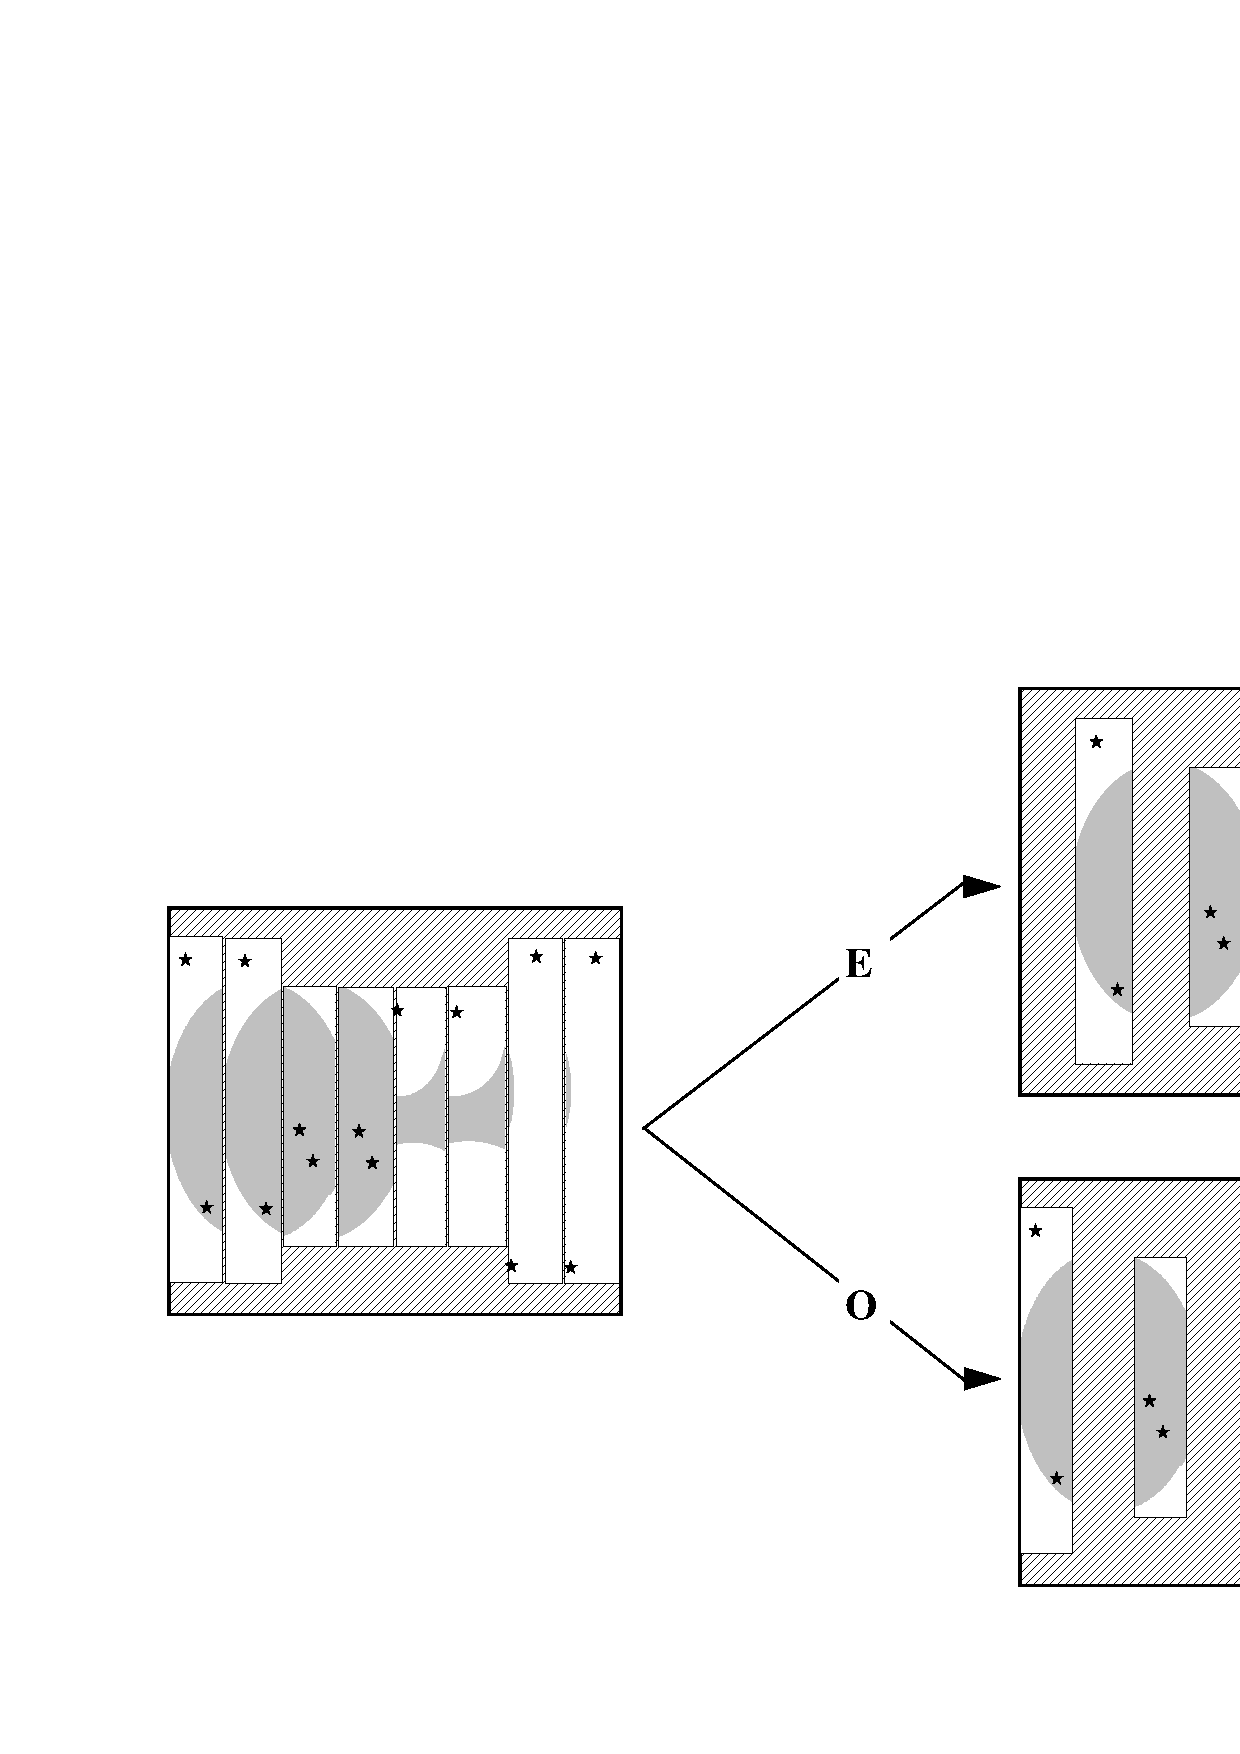
\includegraphics[clip,scale=0.5]{sun223_figures/extract}
  \caption{Extraction of the \emph{O} and \emph{E} ray images.}
  \label{fig:extract}
  \end{center}
  \end{figure}

\subsubsection{Image Alignment}
The arrays holding the extracted $O$ and $E$ ray images now need to be
aligned so that the same pixel in each array corresponds to the same
position on the sky. This can usually be achieved by aligning stars
within the arrays.

\subsubsection{Sky Subtraction}
The intensity of the background night sky now needs to be estimated and
subtracted from each of the aligned arrays. The sky may be polarized, and
so this needs to be performed independently within each of the aligned arrays.

\subsubsection{Estimation of the Stokes Parameters}
The \emph{Stokes parameters} $I$, $Q$ and $U$ are all measures of intensity,
and together provide a useful description of the polarization of the object
being studied. Since $I$, $Q$ and $U$ all have the same units, this
description is generally easier to use than the more obvious description
given by the degree of polarization and the orientation of the plane of
polarization. The mathematical connection between the Stokes parameters
and the sky-subtracted intensities is described \slhyperref{here}{in
appendix }{}{APP:POL}. The output from this stage of the reduction process
is a \emph{Stokes vector} (\emph{i.e.} a set of $I$, $Q$ and $U$ values) for each
measured pixel on the sky.

\subsubsection{Binning of the Stokes Parameters}
One consequence of the fact that the Stokes parameters $I$, $Q$ and $U$
are all measures of intensity, is that they can be binned spatially. This
not only produces less confusing polarization maps (due to the reduced
number of measurements), but also improves the signal-to-noise ratio.

\subsubsection{Calculation of the Degree and Orientation of the Polarization}
The use of Stokes parameters to describe polarization has mathematical
advantages, but is not easy to represent in a graphical manner. For human
interpretation therefore, polarization is usually described by the degree
of polarization, $p$, (\emph{i.e.} the ratio of polarized to total intensity),
and the orientation of the plane of polarization, $\theta$. Note,
$\theta$ is the angle between the plane of polarization and the reference
direction of the polarimeter. To convert this to a position angle on the
sky, the position angle of the reference direction must be known. The
simplest way to derive these parameters from the Stokes parameters is as
follows:

\begin{myquote}
\begin{eqnarray*}
  I_{p} & = & \sqrt{ Q^{2} + U^{2} } \\
  p & = & I_{p}/I \\ \\
  \theta & = & 0.5.\arctan (U/Q)
\end{eqnarray*}
\end{myquote}

where $I_{p}$ is the \emph{polarized intensity}. However, the estimation
of $p$ is complicated by the non-symmetric noise statistics produced by
squaring and adding $Q$ and $U$. For low polarizations, the squaring of
the noise will tend to shift the mean of the distribution of $p$ to
higher values, thus resulting in an over-estimation of $p$. The use of
the following expression for $I_{p}$ reduces the effect of this
statistical bias:

\begin{myquote}
\begin{eqnarray*}
  I_{p} & = & \sqrt{ Q^{2} + U^{2} - \sigma^{2}} \\
\end{eqnarray*}
\end{myquote}

where $\sigma^{2}$ is the variance on $Q$ or $U$ (which are assumed
equal). A description of the statistical behaviour of polarization
parameters is given by Serkowski (\emph{Advances in Astronomy and
Astrophysics}, ed. Z. Kopal, Academic Press, New York, London (1962),
\textbf{1}, 304).

\subsubsection{Display of the Final Polarization Data}
The final polarization parameters are usually presented graphically in
the form of a \emph{polarization map} (see the first page of this document
for an example). Each measurement is represented as a vector parallel to
the plane of polarization. The length of the vector is proportional to
the degree of polarization, which varies from 0\% to 100\%. The Stokes
vectors can be binned to reduce the number of vectors in the map to a
manageable number. The map is often overlayed on a total intensity image
or contour map of the object to emphasize any correlation between the
visual appearance of the object and the morphology of the polarization
map.

\section{\label{SEC:SBPOL}\xlabel{singlebeampolarimetry}Single-beam Polarimetry}
This section gives a brief introduction to the general principles of
single-beam polarimetry. It explains words and concepts used later, and
defines the data model used by POLPACK.

Single waveband polarimetry is described here but the principles can be
extended to imaging spectropolarimetry (see \slhyperref{here}{section }{}{SEC:SPEC}).

\subsection{\label{SEC:SBPOLARIM}The Polarimeter}
An exposure from a single-beam polarimeter consists of an image of the sky
in a single state of polarization. Some form of \emph{analyser} within
the polarimeter removes all but the required state of polarization from
the incoming light, which then goes on to be recorded on a suitable
imaging device such as a CCD camera. A series of exposures is usually taken
with a different state of polarization being recorded by each exposure.
These exposures allow both the degree and orientation of the polarization
to be estimated.

Several analyser arrangements are commonly used. POLPACK can handle data
from the following forms:

\begin{enumerate}

\item A single analyser which passes only light polarized parallel to a
specified axis. The analyser is rotated to measure light polarized in
different directions.

\item Several fixed analysers, each of which passes only light polarized
parallel to its axis. The required analyser is inserted into the light path
to measure light polarized in different directions.

\item A single fixed analyser which passes light polarized parallel to its axis.
A \emph{half-wave plate} is placed in the light path in front of the
analyser to rotate the plane of polarization of the incoming light
before it reaches the analyser. Light polarized in different directions
can thus be measured by rotating the half-wave plate.

A half-wave plate has a preferred axis. Light polarized parallel to this
axis passes through the half-wave plate unchanged. Light polarized
perpendicular to the axis is retarded by half a wavelength. The net
effect of this is to  rotate the plane of polarization of the light so
that the axis of the half-wave plate bisects the angle between the planes
of polarization in the incoming and outgoing light.

This form of polarimeter is shown diagrammatically in
Figure~\ref{fig:singopt}.

  \vspace{2mm}
  \begin{figure}[htb]
  \begin{center}
  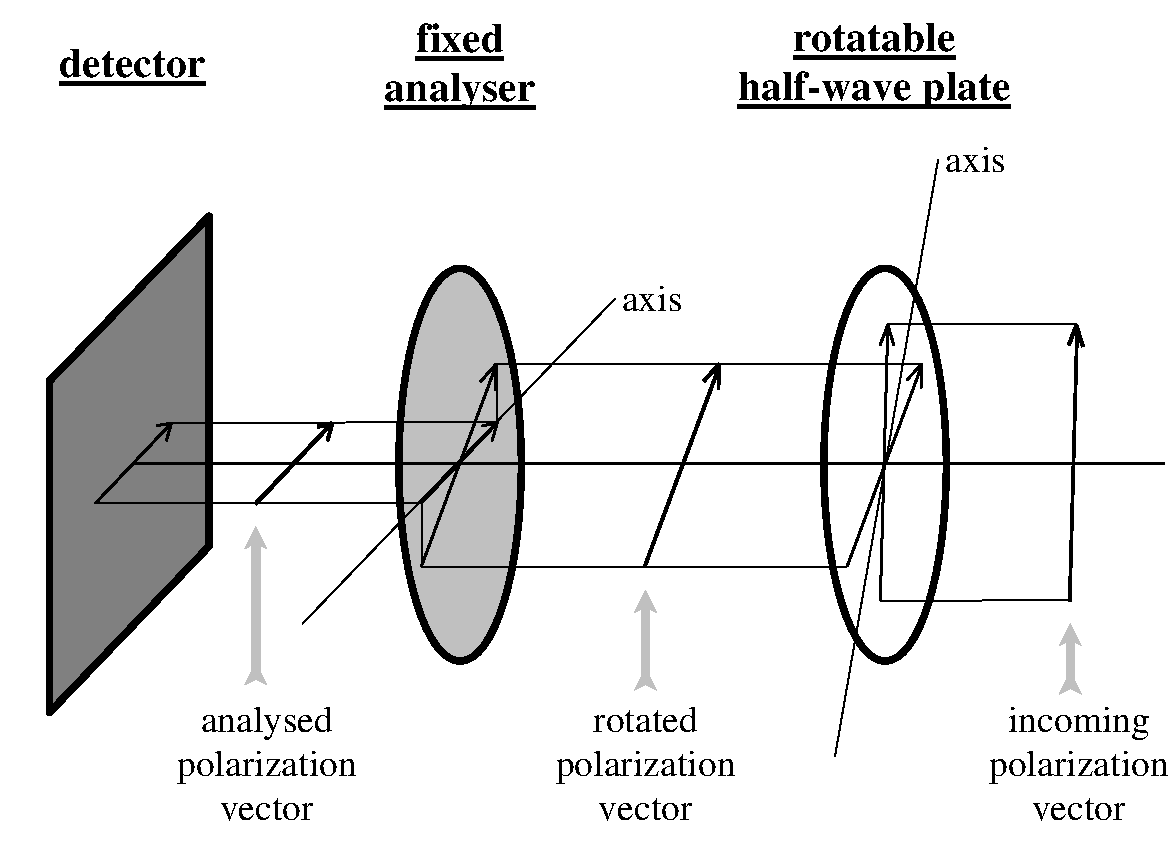
\includegraphics[clip,scale=0.5]{sun223_figures/singopt}
  \caption{The main optical components in a typical single-beam imaging polarimeter.}
  \label{fig:singopt}
  \end{center}
  \end{figure}

\end{enumerate}

There will be a \emph{reference direction} within the focal plane. The
orientation of the rotating analyser or half-wave plate is specified by
giving the
angle between the reference direction and the analyser (or half-wave
plate). In POLPACK, the reference direction is specified by giving the
anti-clockwise angle from the first image axis to the reference
direction. This angle is usually referred to as $ANGROT$, and is specified in
degrees.

The combination of a fixed analyser and a rotating half-wave plate can be
thought of as equivalent to a single rotating analyser, in which the
analyser rotates twice as fast as the half-wave plate. If the
anti-clockwise angle from the reference direction to the half-wave plate
is $WPLATE$, then the \emph{effective analyser position} is given by:

\begin{myquote}
\begin{eqnarray*}
  \phi & = & 2.WPLATE
\end{eqnarray*}
\end{myquote}

This is the angle from the reference direction to a hypothetical analyser
which would give the same effect as the combination of the fixed analyser
and half-wave plate (see Figure~\ref{fig:effan}).

  \begin{figure}[htpb]
  \begin{center}
  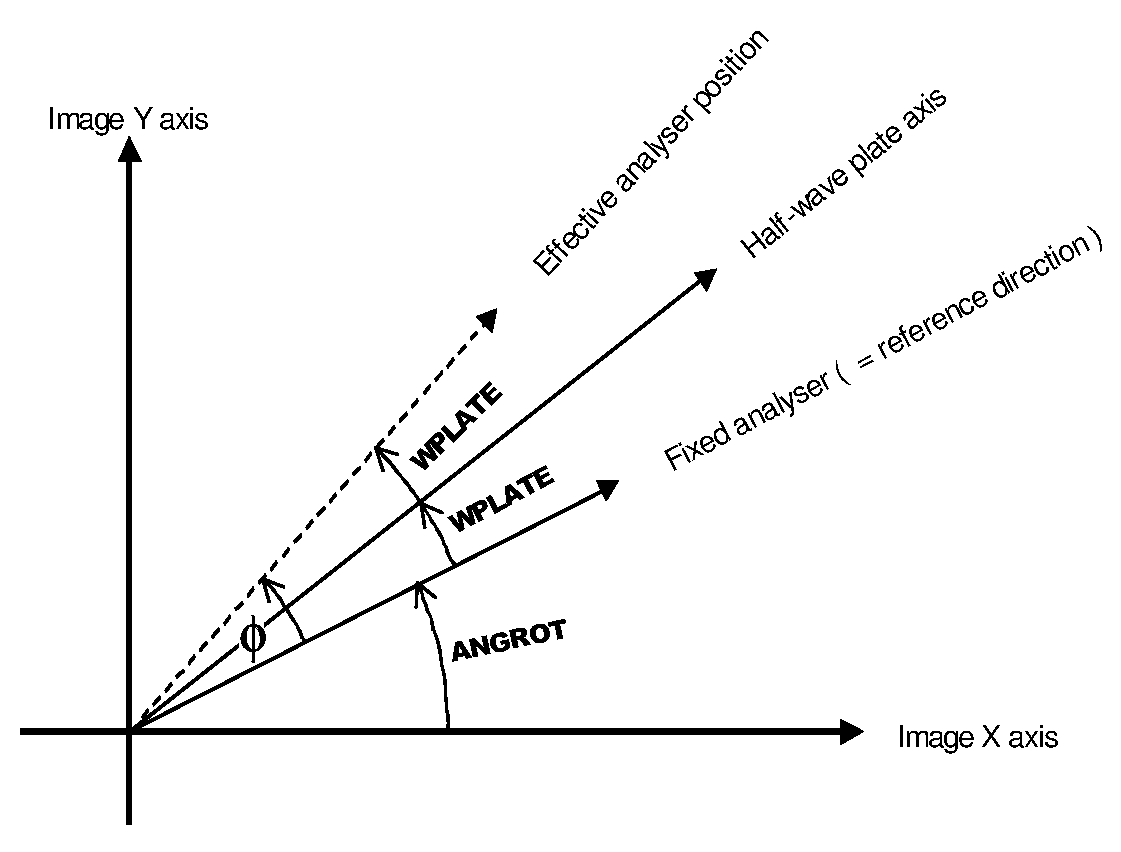
\includegraphics[clip,scale=0.5]{sun223_figures/effan}
  \vspace{4mm}
  \caption{The effective analyser position for a rotating half-wave plate.}
  \label{fig:effan}
  \end{center}
  \end{figure}

The recorded intensity for an analyser position (or effective analyser
position) of $\phi$ will be:

\begin{myquote}
\begin{eqnarray}
\label{EQN:IREC}
  I_{rec} & = & \frac{t}{2}( I + \epsilon.( Q.\cos 2\phi + U.\sin 2\phi ) )
\end{eqnarray}
\end{myquote}

Here $I$, $Q$ and $U$ are the \emph{Stokes parameters} describing the
incoming partially plane polarized light. $I$ is the total intensity,
\emph{i.e.} the sum of the polarized and unpolarized intensities. If a
fraction $p$ of the incoming light is totally plane polarized, then:

\begin{myquote}
\begin{eqnarray*}
  I_{p} & = & I.p \\
  I & = & I_{p} + I_{u}
\end{eqnarray*}
\end{myquote}

where $I_{p}$ is the polarized intensity, and $I_{u}$ is the unpolarized
intensity. Q measures the intensity polarized parallel to the reference
direction, and U measures the intensity polarized perpendicular to the
reference direction. They are given by:

\begin{myquote}
\begin{eqnarray*}
  Q & = & I_{p}.\cos 2\theta \\
  U & = & I_{p}.\sin 2\theta
\end{eqnarray*}
\end{myquote}

Here, $\theta$ is the anti-clockwise angle from the reference direction to
the direction of polarization of the incoming light.

The two other values, $t$ and $\epsilon$ in the above expression for the
record intensity, $I_{rec}$, are the \emph{analyser transmission} and the
\emph{analyser efficiency}. The transmission measures the total
throughput of the analyser, and the efficiency measures the ability of
the analyser to select a single state of polarization. A perfect analyser
would have a value of $1.0$ for both. A perfectly \emph{bad} analyser
such as a piece of high quality glass, would have a transmission of $2.0$
and an efficiency of zero. If you know the transmission and efficiency of
your analysers, then POLPACK can take account of them when estimating the
values of the Stokes parameters, $I$, $Q$ and $U$. If you do not known
them, then don't worry... just use the default values of $1.0$ for both.
These will probably be acceptable since instrument makers usually go to
some trouble to make their analysers as perfect as possible. If in doubt,
you could try re-processing your data with different values for the
analyser transmission and efficiency. This will give you some idea of how
sensitive the final results are to the values used.

\subsection{The Observational Procedure}
At least three exposures with different analyser or half-wave plate
positions are required to estimate the degree and orientation of the
polarization. However, if you can, you should take some extra analyser
positions. Not only does this reduce the noise, but it also allows
consistency checks to be performed, since the recorded intensity should
be a \slhyperref{sinusoidal function}{sinusoidal function (see equation }
{)}{EQN:IREC} of analyser or half-wave plate position. POLPACK provides
facilities to reject data values which are more than a given distance from
the best fitting sine curve (\slhyperref{more details here}{see appendix }{}
{APP:SNGBM}).

\subsection{The Data Reduction}
There are many similarities between the reduction of single-beam
dual-beam data. The basic differences are that each target exposure
contains only a single image of the sky, instead of the two images
produced by a dual-beam polarimeter, and that rotation between images is
allowed. The various steps involved are
summarised below. For more details \slhyperref{go here}{see section }
{}{SEC:DBRED}. Details of how POLPACK can be used to implement these
ideas in practice are given in later sections of this document.

\section{\label{SEC:SPEC}\xlabel{spectropolarimetrydatareduction}Spectropolarimetry
Data Reduction}
POLPACK assumes that spectropolarimetry data is identical to single
waveband polarimetry data, except that each data file has an extra pixel
axis giving spectral channel. Thus, analysed intensity data is stored in a
3 dimensional NDF in which the first two pixel axes are spatial axes, and the
third axis gives the spectral channel. Stokes vectors are stored in a 4
dimensional NDF in which axes 1 and 2 are spatial, axis 3 is spectral, and
axis 4 corresponds to Stokes parameter (1=I, 2=Q, 3=U, \emph{etc}).
Vector catalogues have an extra column (``Z'') giving the spectral channel.

The data in each spectral channel is processed as if it were data from a
single waveband polarimeter (\emph{i.e.} the processing of each spectral
channel is largely independent of the processing of the other spectral
channels). The one exception to this is that the \htmlref{POLBIN}{POLBIN}
application can bin adjacent spectral channels, as well as binning
adjacent spatial pixels.

In general, and unless otherwise stated, all POLPACK applications will handle
spectropolarimeter data in the same way that it handles single waveband
data. However, for ``historical reasons'' you may find a bias towards single
waveband data in the documentation. References to \emph{intensity images}
should be understood as meaning \emph{intensity images or cubes}, and
\emph{Stokes cubes} should be taken as \emph{Stokes cubes or 4D
hyper-cubes}.

\section{\label{SEC:POLRED}\xlabel{datareductionusingpolpack}Data Reduction Using POLPACK}
This section gives a detailed description of the steps involved in using
POLPACK to produce a vector map from single-beam or dual-beam polarimetry
or spectropolarimetry data. It is assumed that the data conforms to the model outlined in one
of the two previous sections. An over-view of the data reduction process
is given in Figure~\ref{fig:dataflow}.

  \begin{figure}[htpb]
  \begin{center}
  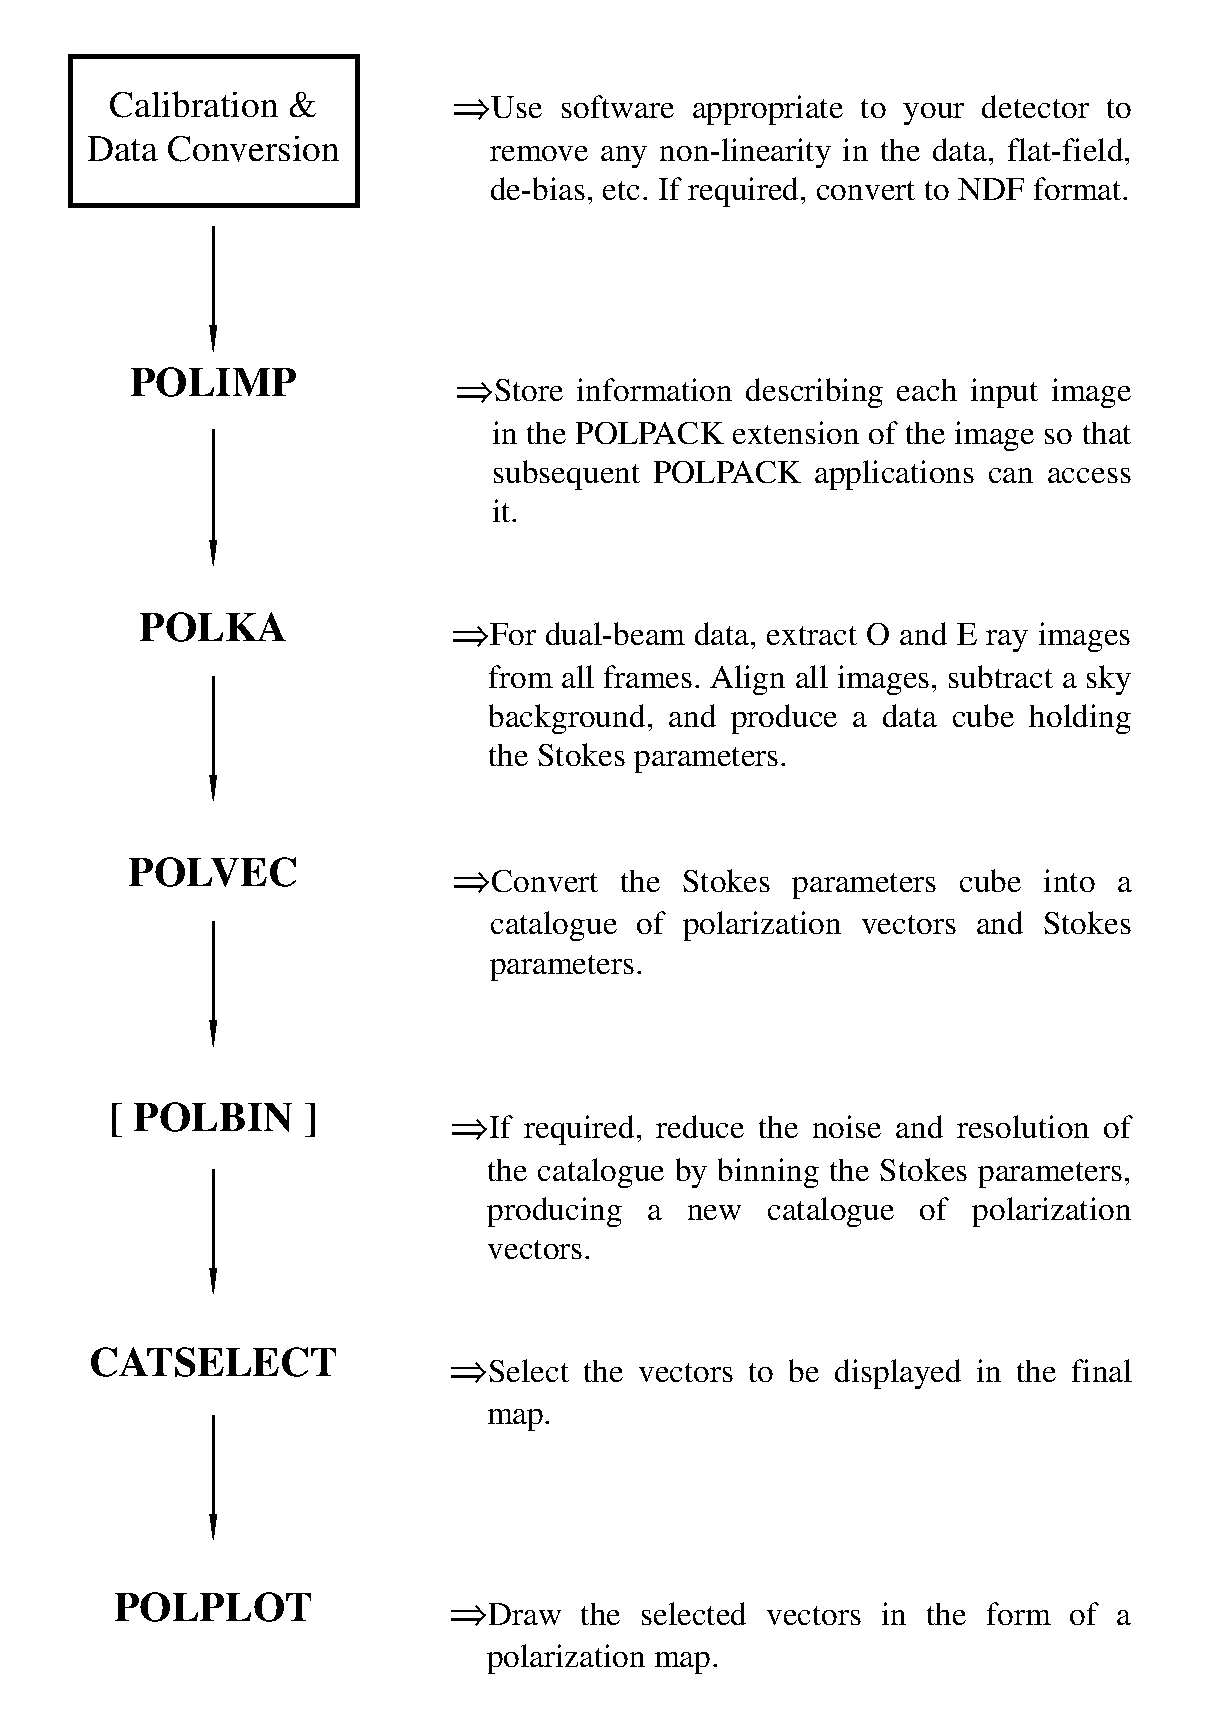
\includegraphics[clip,scale=0.7]{sun223_figures/dataflow}
  \vspace{4mm}
  \caption{The main steps in the production of a polarization map.}
  \label{fig:dataflow}
  \end{center}
  \end{figure}

All POLPACK applications use standard Starlink subroutine libraries for
accessing parameters, producing graphics, reporting errors, \emph{etc}. They
therefore look and feel very similar to applications in other Starlink
packages such as KAPPA and CCDPACK. The following sections in
\xref{SUN/95}{sun95}{} (the KAPPA manual) should therefore be consulted for general
information about these issues:

\begin{itemize}
\item ``\xref{Parameters}{sun95}{se_param}''
\item ``\xref{Graphics Devices and Files}{sun95}{se_graphdev}''
\item ``\xref{Plotting Styles and Attributes}{sun95}{se_style}''
\item ``\xref{Data Structures}{sun95}{se_datastr}''
\item ``\xref{NDF Sections}{sun95}{se_ndfsect}''
\item ``\xref{NDF History}{sun95}{se_ndfhistory}''
\item ``\xref{The Graphics Database}{sun95}{se_agitate}''
\item ``\xref{Using World Co-ordinate Systems}{sun95}{se_wcsuse}''
\item ``\xref{Procedures}{sun95}{se_procedures}''
\end{itemize}

\subsection{\label{SEC:CONVERT}\xlabel{formatconversion}Format Conversion}

The first step is to ensure that your data files are in a format which
POLPACK can process. The native data format used by POLPACK is the
Starlink \xref{NDF}{sun33}{} format (note, NDF structures are usually
stored in files with a file type of \verb+.sdf+). If your data is already
in this format, then you can proceed immediately to the next step. Otherwise,
you have two options:

\begin{enumerate}

\item You can convert your data files into NDF format explicitly at the
beginning, and use the NDF versions there-after. The \xref{CONVERT}{sun55}{}
package (see SUN/55) provides facilities for converting to and
from most common astronomical data formats. For instance, if your data is
in the form of a set of FITS files, you could use commands similar to the
following to convert them into NDFs:

\begin{terminalv}
% convert
% fits2ndf "*.fit" "*"
\end{terminalv}

Note that the \texttt{\%} represents the C-shell prompt and should not be typed.
The first command initialises the commands required to use the CONVERT
package. The second command converts all FITS files with a file type of
\verb+.fit+ within the current directory, into equivalent NDFs with the
same file names, but a file type of \verb+.sdf+\footnote{The double quotes
are needed to prevent the asterisks being expanded by the shell. The
expansion of these file templates is performed internally, within
fits2ndf.}. The \verb+.sdf+ files can then be given as inputs to
any application from POLPACK, CCDPACK or KAPPA.

\item Alternatively, you can rely on the facilities of the NDF library to perform
automatic on-the-fly data conversions as and when necessary. Using this
technique, POLPACK, CCDPACK and KAPPA all appear to process your data files
directly without you needing to do any explicit data conversion. All you
need to do to enable these facilities is to initialise the CONVERT
package using the single command:

\begin{terminalv}
% convert
\end{terminalv}

If you adopt this approach, you may still see references to ``NDFs''
appearing on the screen. There is usually no significance in the use of
the term ``NDF'' in this context (unless there are indications to the
contrary), and you should understand these as referring to your own
non-NDF data files.

\end{enumerate}

For spectropolarimetry data, the spectral channel must vary along pixel
axis 3, and pixel axes 1 and 2 must be spatial axes. The KAPPA
application \xref{PERMAXES}{sun95}{PERMAXES} can be used to rearrange
axes into the required order. If your data is one dimensional
(\emph{i.e.} has no spatial coverage) then you can use PERMAXES as
follows to add two spatial axes each covering a single pixel:

\begin{terminalv}
% permaxes in="data-1d(,1,1)" out=data-3d perm="[2,3,1]"
\end{terminalv}

where \texttt{data-1d.sdf} is the 1-dimensional input file, and \texttt{data-3d.sdf} is the 3-dimensional output file. The section specifier
``\texttt{(,1,1)}'' indicates that \texttt{data-1d} should be treated as if it
had 2 extra trailing axes each spanning a single pixel. PERMAXES then
rearranges the axes so that the spectral axis (previously axis 1) becomes
the last axis (axis 3). Of course, since there is no spatial coverage,
you will not be able to display such data using \htmlref{POLPLOT}{POLPLOT}
(use \htmlref{POLIMAGE}{POLIMAGE} and KAPPA \xref{LINPLOT}{sun95}{LINPLOT}
instead).

\subsection{\label{SEC:CCDPACK}Corrections for Instrumental Effects}
POLPACK expects your data to be calibrated so that the pixel values are
proportional to the analysed intensity. You should therefore correct your
data for any known instrumental effects such as non-linearity, variation
of sensitivity across the detector, zero point offsets, \emph{etc.}, before
proceeding to use POLPACK. The details will obviously depend on your
detector, but if you are using a CCD camera, then the \xref{CCDPACK}{sun139}{}
package (see SUN/139) will usually be able to perform these corrections.

If you are using dual-beam data, and target exposures are available at
half-wave plate positions of
45.0\dgs\ and 67.5\dgs\ (as well as 0\dgs\ and 22.5\dgs), then POLPACK can
make corrections for the following effects when calculating the Stokes
vectors:

\begin{enumerate}
\item Differences in exposure times between the target exposures
\item A constant difference in sensitivity between the $O$ and $E$ ray
channels.
\end{enumerate}

These effects therefore do not need to be calibrated out of the raw data.

One aspect of calibration common to most detectors is flat-fielding. If
your flat-fields are obtained in polarized light (such as produced by
reflection or scattering, for instance), then the mean signals measured
in the $O$ and $E$ ray images of dual-beam data will be different. When
such a flat-field
is used to calibrate your target exposures, these different mean levels
will introduce an apparent difference in sensitivity between the $O$ and
$E$ ray channels. If the \emph{same} flat-field is used for all target
exposures, then this difference in sensitivity will be constant and can
be removed while calculating the Stokes parameters (provided you have
target exposures at half-wave plate positions of 0, 22.5, 45 and 67.5
degrees). \slhyperref{Go here for}{Appendix }{ contains}{APP:FFCOR} a
mathematical description of the flat-fielding process for dual-beam data,
and the corrections applied by POLPACK when calculating the Stokes parameters.

Whether you are using dual-beam or single-beam data, \emph{do not forget to
use the same flat-field to correct \textbf{all} target exposures}. This
will usually be a master flat-field formed by co-adding several
individual flat-field exposures. This reduces the noise in the master
flat-field. This is important for two reasons:

\begin{enumerate}
\item Any noise in the flat-field gets passed directly into the final results.
\item Any noise in the flat-field appears in each of the flat-fielded
intensity images, resulting in a degree of correlation between the noise in
these images. This can cause any variance estimates for the final
polarization parameters (see next paragraph) to be wrong. This is because
the variance calculations assume that there is no correlation between the
noise in different images.
\end{enumerate}

Another aspect of instrumental calibration is the estimation of the
uncertainty on every pixel value. If you know the noise characteristics
of your detector, you may be able to store this information with your
data in the form of an NDF VARIANCE component. This is an array
holding an estimate of the variance at every pixel in your data. If
present, POLPACK will process this information to obtain estimates of the
uncertainty in the final polarization parameters. If you use CCDPACK to
calibrate your data, then the \xref{DEBIAS}{sun139}{DEBIAS} application
can be used to create a VARIANCE component.

If you are using single-beam data, there is an option to estimate the
variances associated with the input data while calculating the Stokes
vectors.
This enables variances to be found for the Stokes vectors even if your
input data has no usable variance information. \slhyperref{Go here}{See section }
{}{APP:SNGBM} for details.

\subsection{\label{SEC:START}\xlabel{startup}Starting up POLPACK}

The applications within POLPACK are made available from the C shell using the
command:
\begin{terminalv}
% polpack
\end{terminalv}

This command must be issued before attempting to use any POLPACK
applications. POLPACK is also available from the \xref{ICL}{sg5}{}
(see SG/5) command language, and the IRAF cl.

\subsection{\label{SEC:IMPORT}Importing Header Information}
POLPACK needs to know certain items of header information about each of
the supplied data files. These include the half-wave plate position, the
orientation of the reference direction, \emph{etc}. Different instruments may
store this information in different ways, and for this reason, POLPACK
includes an application which finds the required items of information and
stores them away in a standard place within the data file from where the
other POLPACK applications can extract them when needed. This standard
place is known as the ``POLPACK extension''. The process of copying this
information from its original, instrument specific location, into the
POLPACK extension is known as ``importing'' the data, and is performed by
the \htmlref{POLIMP}{POLIMP} application\footnote{Once imported, the POLPACK
extension is propagated through the entire data reduction sequence, with
new items being added at various points to describe the intermediate
stages of processing.}, or the \htmlref{POLEXT}{POLEXT} application (if
you have no FITS headers available).

You tell POLIMP where to find each required item of information by
supplying it with a ``control table''. This is a text file containing a
line for each item of information to be imported into the POLPACK
extension. Each such item has a name by which other POLPACK applications
refer to it (these are described \slhyperref{here}{in
appendix }{}{APP:POLEXT}). As well as the name of a POLPACK extension
item, each line of the control table should contain a description of where to
obtained the corresponding value. This description is given in terms of
FITS keywords. For instance, the line

\begin{terminalv}
WPLATE HWPANG
\end{terminalv}

tells POLIMP to find the value of the FITS keyword \verb+HWPANG+ and
store it as item ``WPLATE'' in the POLPACK extension (this is the
half-wave plate position angle).

If your data are supplied in the form of a set of FITS files, then the
\verb+HWPANG+ value would simply be obtained from the primary header. If your
data is supplied in the form of a set of NDF structures, then the value
would be read from the FITS extension in the NDF structure (which should
have been created by the data acquisition system). For other data formats,
the origin of the keyword value depends on how the data conversion is
performed. \xref{SUN/55}{sun55}{} contains details of how FITS keywords
are created from foreign data files.

The POLIMP control table also allows POLPACK extension items to be
derived from one or more FITS keyword values, combined together to form a
Fortran-like mathematical expression. For instance, this may be useful if
the FITS keyword uses a different set of units, or has a different sign
convention. When used in this way, each FITS keyword must be ``declared''
earlier in the control table. This declaration tells POLIMP what sort of
data values the keyword can take. For instance:

\begin{terminalv}
_REAL  ROTA
ANGROT 57.29578*ROTA
\end{terminalv}

converts the value of the FITS keyword \verb+ROTA+ from radians to
degrees, and assigns the result to the item ANGROT.
The first line informs POLIMP that the keyword \verb+ROTA+ should be
treated as a single precision floating point value. The recognized data
types are:

\begin{quote}
\begin{description}
\item[\texttt{\_BYTE}]		- Single byte signed integer values.
\item[\texttt{\_CHAR}]		- Character strings.
\item[\texttt{\_DOUBLE}]       	- Double precision floating point values.
\item[\texttt{\_INTEGER}]	- Single precision integer values.
\item[\texttt{\_REAL}]		- Single precision floating point values.
\item[\texttt{\_WORD}]		- Two byte signed integer values.
\end{description}
\end{quote}

See the description of the \htmlref{POLIMP}{POLIMP} application for
further details of the syntax of the control table.

There is also a \htmlref{POLEXP}{POLEXP} application which reverses the
importing process. It copies the information stored in the POLPACK
extension into named FITS keywords. The primary purpose of POLEXP is
to allow the automatic format conversion facilities of the NDF library to
convert a POLPACK NDF structure back into a foreign data file.
It is generally not necessary for users to call POLEXP explicitly.

The \htmlref{POLEXT}{POLEXT} application allows the contents of the
POLPACK extension to be set to explicit values supplied by the user. This
can be useful if your data does not contain any FITS headers. POLEXT will
also list the contents of the POLPACK extension. If your data is stored
in NDF format, you can also use the \xref{\texttt{hdstrace}}{sun102}{}
command to list the contents of the NDF extension. For instance, to check
the contents of the POLPACK extension in the NDF \verb+partproc.sdf+, do:

\begin{terminalv}
% hdstrace partproc.more.polpack
\end{terminalv}

\subsection{Reference Directions}
The reference direction within each image is recorded by adding a new
co-ordinate Frame to the World Co-ordinate System (WCS) information
stored with the image (see \slhyperref{here}{section }{}{SEC:WCS}). The new
Frame has the Domain name \verb+POLANAL+,
and its first axis is parallel to the reference direction. This Frame
will be updated by any POLPACK application which produces a change in the
orientation of the reference direction. This will happen
for instance if \htmlref{POLKA}{POLKA} introduces a rotation into the
images during the alignment process\footnote{Rotation is currently only
possible when processing single-beam data.}. If you process your images
using applications from another package, then be aware that the POLANAL Frame
may be lost or invalidated. Basically,
you will probably be safe if you only use packages which correctly
propagate WCS information in form of Starlink AST FrameSets (see
\xref{SUN/210}{sun210}{}). KAPPA, for instance, is such a package.

You specify the reference direction when you run POLIMP or POLEXT by
giving a value for the ANGROT item (the anti-clockwise angle in degrees
from the first image axis to the reference direction). In versions of
POLPACK prior to V2.0, ANGROT was stored explicitly as a floating point
value within the POLPACK extension. As of V2.0, ANGROT is no longer
stored in the POLPACK extension. Instead, its value is implied by the
orientation of the \verb+POLANAL+ Frame within the WCS information.
However, you can consider this an ``implementation detail'' -- as far as
the general user is concerned, ANGROT can be treated like any of the
genuine extension items. In particular, it can be set or examined using
POLIMP, POLEXT and POLEXP just like any other POLPACK header item.

\subsection{Creation of Stokes Parameters}
The creation of Stokes vectors from the calibrated, imported
target exposures involves the following steps:

\begin{itemize}
\item The extraction of the $O$ and $E$ ray images in each target
exposure into separate files (dual-beam data only).
\item The alignment of all images, so
that a given pixel position corresponds to the same place on the sky in
all images.
\item The subtraction of a sky background from each image.
\item The calculation of the Stokes vectors from these sky-subtracted
images.
\end{itemize}

The first three of these steps can be performed using applications from
KAPPA and CCDPACK, and the final step is performed by the POLPACK
application \htmlref{POLCAL}{POLCAL}. However, this is a fairly involved
process since the available applications are somewhat low-level. For this
reason, POLPACK includes a tool called \htmlref{POLKA}{POLKA} which
simplifies the process. POLKA is effectively a script which calls the
KAPPA, CCDPACK and POLPACK applications required to perform all four of
the steps listed above\footnote{The final step - calculating the Stokes
parameters - is optional. This allows POLKA to be used as a general
purpose image alignment tool for non-polarimetric data.}. While some
options are provided to allow the user to customise the exact recipe
used, POLKA does not provide as much versatility or control over the
processing as would be available if the individual applications were
called ``by hand''. If you hit a problem which POLKA cannot handle, then
you may need to adopt this alternative approach.

One specific restriction on POLKA is that it can only be used with
2-dimensional intensity images (\emph{i.e.} not 3-dimensional
spectropolarimetry data). To create Stokes vectors from 3-dimensional
intensity cubes, the cubes must first be aligned in both the spatial and
the spectral domain (\emph{e.g.} using CCDPACK and KAPPA applications
``by hand''), and then \htmlref{POLCAL}{POLCAL} should be used to create
a 4-dimensional hyper cube containing Stokes vectors.

POLKA requires you to identify the following features within the supplied
images:

\begin{itemize}
\item The areas containing the $O$ and $E$ ray images (dual-beam data only).
\item The sky areas.
\item Any star-like features which can be used to align the images.
\end{itemize}

A Graphical User Interface (GUI) is created for this purpose, including
an image display area in which any of the input images may be displayed,
and controls to select any of the above features (see Figure
~\ref{fig:polka}). Note, if you find the image display area uncomfortably
small, it can be made larger by assigning a suitable value to the DPI
parameter when POLKA is started. Once the required features have been
supplied, POLKA commences the processing of the supplied data frames.
This may take a significant length of time depending on your hardware,
and the size and number of your images. A window displays the progress
being made during this phase.

  \begin{figure}[htpb]
  \begin{center}
  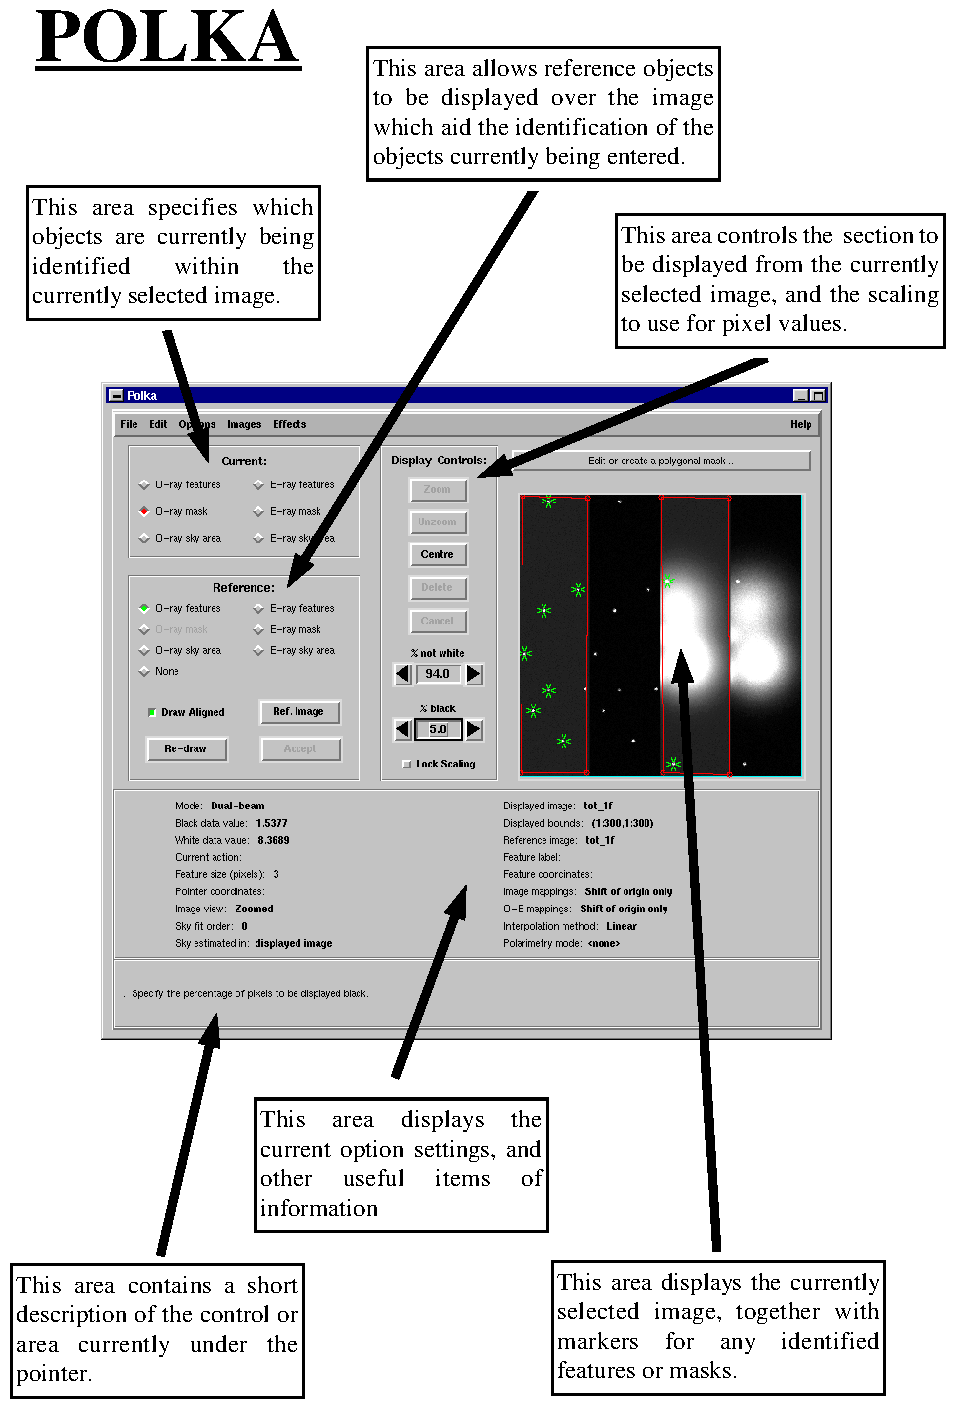
\includegraphics[clip,scale=0.85]{sun223_figures/polka}
  \vspace{4mm}
  \caption{The Graphical User Interface presented by POLKA.}
  \label{fig:polka}
  \end{center}
  \end{figure}

Once complete, a 3D cube is created in which the x-y plane corresponds to
pixel positions within the extracted, aligned intensity images. Each
plane in the cube contains a single Stokes parameter. The lowest plane is
always the total intensity. The other planes contain either Q and U for
linear polarization, or V for circular polarization\footnote{POLPACK can
currently only measure circular polarization for dual-beam data.}. In
addition, the separate aligned, sky-subtracted intensity images on which
the Stokes parameters were based may be saved once the processing is
complete.

The reference direction (see \slhyperref{this section}{section }
{}{SEC:SBPOLARIM}) for the Stokes vectors in the output cube will
not in general be the same as the reference direction in the input
intensity images. The output reference direction is chosen as follows:

\begin{itemize}
\item If the input data has World Co-ordinate System (WCS) information
which describes a celestial co-ordinate system such as RA/DEC, galactic
longitude/latitude, \emph{etc.}, then the reference direction in the output cube
will be north within the same celestial co-ordinate system.
Instructions on setting up such WCS information is available
\slhyperref{here}{in section }{}{SEC:WCS}.

\item If the input data does not contain WCS information for a celestial
co-ordinate system, then the reference direction will be the second pixel
axis within the image (\emph{i.e.} ``Y'', or ``upwards'' if the image is
displayed normally).
\end{itemize}

The POLKA application has many parameters. The values used for some of
these may be changed from within the GUI. However, some may not be
changed and should be assigned appropriate values when invoking POLKA.
Of these, the most important will usually be:

\begin{quote}
\begin{description}
\item [IN]	- A list of the input target frames. These should have been
calibrated and imported. The list may be supplied in several forms
(described \slhyperref{here}{in section }{}{SEC:GRPEXP}).
\item [MODE]	- Indicates what sort of polarization you are measuring. It
can be ``CIRCULAR'' or ``LINEAR''.
\item [OUT]	- If you have single-beam, or non-polarimetric data, this
parameter is used to obtain a list of the output images to receive the
aligned, sky-subtracted images. If a null value (!) is supplied, these
images are not saved. For dual-beam data, parameters OUT\_E and OUT\_O
are used instead.
\item [OUT\_E]	- A list of the output images to receive the extracted,
aligned, sky-subtracted $E$ ray images. If a null value (!) is supplied,
these images are not saved. Only used in dual-beam mode.
\item [OUT\_O]	- This is like OUT\_E, but refers to the $O$ ray images
instead of the $E$ ray images. Only used in dual-beam mode.
\item [OUT\_S]	- The name of the output cube to receive the Stokes
parameters. If a null value (!) is supplied, no Stokes parameters are
created.
\item [POL]	- This should be set to FALSE if you want to use POLKA as a
general purpose image alignment tool for non-polarimetric data. If this
is done, the aligned, sky-subtracted images should be specified using parameter
OUT (parameters OUT\_S, OUT\_E and OUT\_O are then not used). In this mode,
the supplied images are treated like $O$ ray images, and the controls
related to the $E$ ray images are disabled.
\item [SKYFRAMES] - POLKA provides two methods of sky subtraction. If a
list of frames is supplied for parameter SKYFRAMES, then these frames are
subtracted pixel-by-pixel from the target intensity frames. If a null
parameter value (!) is supplied for SKYFRAMES, then you must use the GUI to
identify areas of sky within each of the input target frames. A smooth
surface is then fitted to these areas and used as the sky background.

\end{description}
\end{quote}

A separate guide is available describing POLKA in detail. It
contains a step-by-step tutorial, detailed descriptions of
each control in the GUI, answers to some common questions, \emph{etc}. It may be
accessed using the \verb+Help+ menu within the GUI. When POLKA is
activated, the tutorial is automatically displayed in a WWW browser (this
may be disabled using the STARTHELP parameter when running POLKA). If you
are new to POLKA, it is  a good idea to work your way through the
tutorial first.


\subsection{\label{SEC:DISP}Displaying the Results}
Linear polarimetry results are usually expressed in terms of the
percentage polarization and the orientation of the plane of polarization.
Vectors may be used to represent these quantities graphically. The
following POLPACK applications can be used to produce a map of vectors
describing the polarization at different points on the sky:

\begin{quote}
\begin{description}
\item [\htmlref{POLVEC}{POLVEC}] - This converts a 3 or 4D NDF containing
Stokes parameters (such as produced by POLKA or POLCAL) into a catalogue
of polarization vectors containing the following columns:

\begin{quote}
\begin{description}
\item [X] - X pixel co-ordinates within the supplied cube.
\item [Y] - Y pixel co-ordinates within the supplied cube.
\item [Z] - Z pixel co-ordinates within the supplied cube (only produced
            for spectropolarimetry data).
\item [I] - Total intensity.
\item [Q] - Stokes parameter Q.
\item [U] - Stokes parameter U.
\item [P] - Percentage polarization.
\item [ANG] - The anti-clockwise angle from the reference direction to
the plane of polarization, in degrees.
\end{description}
\end{quote}

For circular polarimetry, the Q and U columns are replaced by a single V
column. If variance information is available (see \slhyperref{here}{section
} {}{SEC:CCDPACK}) then columns are also produced holding the standard
deviations associated with each of the above quantities (except X, Y and
Z). Each pixel in the x-y plane of the supplied cube produces one or more
rows in the catalogue, the number being equal to the number of spectral
channels in the data. So for single waveband polarimetry, the catalogue
will contain one row for each pixel in the x-y plane, but for
spectropolarimetry data with (say) 100 spectral channels, there will be
100 rows for each pixel in the x-y plane. The reference direction for the
$Q$, $U$ and $ANG$ columns is chosen in the same way as when producing
the Stokes vectors (\emph{i.e.} north, if WCS information is available to
define north, or the second image axis otherwise).

POLVEC can also produce a set of 2 or 3D NDFS holding the above quantities.

\item [\htmlref{POLBIN}{POLBIN}] - This accepts a catalogue containing Stokes
parameters as input (such as produced by POLVEC), and creates a new
output catalogue in the same format, but containing fewer rows (\emph{i.e.}
fewer polarization vectors). The output catalogue is formed by binning the
Stokes vectors in the input catalogue within a grid of equally sized
rectangular bins. Corresponding values for the P and ANG columns are
calculated on the basis of the binned Stokes parameters.
Spectropolarimetry data can be binned independently in the spatial and
spectral axes.

\item [\htmlref{POLPLOT}{POLPLOT}] - This displays a map of polarization
vectors in a single spectral channel, obtained from a catalogue produced
by POLVEC or POLBIN (the catalogue must contain more than a single
spatial position). If the data contains more than one spectral channel,
the specific spectral channel to display can be selected. If the map is
drawn over an existing picture, then the vectors can be aligned with the
previously displayed picture.

\end{description}
\end{quote}

In addition, the catalogues produced by POLBIN and POLVEC can be examined
and interactively edited using the polarimetry toolbox within
\xref{GAIA}{sun214}{} (SUN/214).

Since the polarization parameters are stored in a catalogue, the
\xref{CURSA}{sun190}{} package (see SUN/190) can be used to
examine and manipulate them. One particularly useful facility within
CURSA is the \xref{CATSELECT}{sun190}{SELECT} application, which
allows rows within a catalogue to be selected on the basis of an
arbitrary mathematical expression. For instance the following commands
create a new catalogue called \verb+selcat.FIT+ which contains all the
vectors from \verb+bincat.FIT+ for which the polarization is less than
30\% and has a standard deviation less than 5\%:

\begin{terminalv}
% cursa
% catselect catin=bincat catout=selcat norejcat seltyp=e "expr='p<30 & dp<5'"
\end{terminalv}

The \xref{XCATVIEW}{sun190}{XVIEW} application allows you to examine the
data in a catalogue, using a Graphical User Interface to control the
operation and display the results.

Note, the \htmlref{POLIMAGE}{POLIMAGE} application can be used to extract
the values from a specified column of a catalogue into an image. The image
can be either a simple 1-dimensional list of the column values, or it can
be a 2-dimensional image in which the spatial position of each value is
retained. In this case, the image is formed by binning the column values
into a grid of pixels.

A typical recipe for using the above applications (together with KAPPA)
to display a spatial vector map would involve the following steps:

\begin{enumerate}

\item Convert the 3D NDF in file \verb+cube.sdf+ containing Stokes vectors
(created by POLKA) into a catalogue stored in file \verb+cat.FIT+:

\begin{terminalv}
% polvec cube cat
\end{terminalv}

\item Bin the catalogue to reduce the noise and decrease the density
of vectors in the final map. The bins used in this example are 8 by
8 pixels (measured in
the x-y plane of the Stokes parameter NDF \verb+cube.sdf+), and the
Stokes parameters are combined using a median. The binned catalogue is
stored in file \verb+bincat.FIT+:

\begin{terminalv}
% polbin cat bincat 8 method=med
\end{terminalv}

\item Create a new catalogue (in file \verb+selcat.FIT+) containing just
the vectors with polarizations of less than 50\% and standard deviations of
less than 5\%:

\begin{terminalv}
% cursa
% catselect catin=bincat catout=selcat norejcat seltyp=e "expr='p<50 & dp<5'"
\end{terminalv}

\item \label{STEP:DEVICE} Start up KAPPA, and then select the graphics
device and the image display device (both are set to an X windows display
in this example):
\begin{terminalv}
% kappa
% gdset xwindows
% idset xwindows
\end{terminalv}

\item Clear the screen:
\begin{terminalv}
% gdclear
\end{terminalv}

\item \label{STEP:PICDEF} Create a ``picture'' to contain a grey-scale display of the total
intensity. A picture is an area of the screen in which subsequent graphics
will appear. The one we create here is centred on the screen and occupies
three quarters of its height and width. This leaves a border available
for annotation round the display:
\begin{terminalv}
% picdef mode=cc fraction=0.75
\end{terminalv}

\item \label{STEP:DISPLAY} Display the total intensity image contained in the bottom plane of
the Stokes vector cube, and ensure it is displayed with the standard
monochrome colour table:
\begin{terminalv}
% display "cube(,,1)" mode=per percentiles="[5,95]"
% lutgrey
\end{terminalv}

\item \label{STEP:PICLIST} Re-select the ``base picture''. This is a
picture which corresponds to the whole screen. We need to do this because
output from graphics applications such as POLPLOT is usually restricted
to the current picture. At the moment, the current picture is the one
created by PICDEF above which contains the grey-scale image. We want the
key produced by POLPLOT to appear outside this picture. We therefore need
to select the base picture so that POLPLOT has room for the key within
the current picture:
\begin{terminalv}
% piclist picnum=1
\end{terminalv}

\item \label{STEP:POLPLOT} Display the vector map, retaining the existing picture so that the
vectors appear in alignment with the previously displayed total intensity
image. The vectors are drawn in blue. A default scale will be used for the
vectors, but this can be over-ridden if necessary by specifying a value for
parameter \htmlref{VSCALE}{POLPLOT}:
\begin{terminalv}
% polplot selcat noclear "style='colour(vect)=blue'"
\end{terminalv}

\end{enumerate}

The above basic recipe can be modified in many ways. For instance:

\begin{itemize}

\item If you want to display only a sub-section of the map, specify the
sub-section in step \ref{STEP:DISPLAY} by including bounds for the
first and second axes of input cube. For instance, to restrict the
display to X pixel co-ordinates 50 to 100, and Y pixel co-ordinates 300
to 380, do:

\begin{terminalv}
% display "cube(50:100,300:380,1)" mode=per percentiles="[5,95]"
\end{terminalv}

\item If you do not want the vectors to be overlaid on a total
intensity image, then omit steps \ref{STEP:PICDEF} and
\ref{STEP:DISPLAY}, and remove the \verb+noclear+ setting from the
POLPLOT command line in step \ref{STEP:POLPLOT}.

\item If you want the vectors overlaid on a contour map instead of a
grey-scale image, replace step \ref{STEP:DISPLAY} with:

\begin{terminalv}
% contour "cube(,,1)" mode=per percentiles="[90,93,96,99]" noaxes nokey
\end{terminalv}

\item If you want your output in the form of a PostScript file, there is
an extra step. This is because graphics applications such as DISPLAY,
CONTOUR, POLPLOT, \emph{etc.}, produce separate output PostScript files which
then need to be combined into a single file using the
\xref{\texttt{psmerge}}{sun164}{} command. In step \ref{STEP:DEVICE},
specify the device as \verb+epsf_l+ (Encapsulated PostScript, landscape
mode) instead of \verb+xwindows+. The first graphics applications to be
run will then write its output to the file \verb+gks74.ps+, and
subsequent graphics applications will write their output to files
\verb+gks74.ps.1+, \verb+gks74.ps.2+, \emph{etc.}\footnote{The sequence number
added to the end of the file name is always one higher than in any
existing files.}. To produce a contour map with overlaid vectors, replace
steps \ref{STEP:DISPLAY} and \ref{STEP:POLPLOT} with:

\begin{terminalv}
% rm gks74.ps*
% contour "cube(,,1)" mode=per percentiles="[90,93,96,99]" noaxes nokey
% mv gks74.ps.1 contour.ps
% polplot selcat noclear
% mv gks74.ps.1 polplot.ps
% psmerge polplot.ps contour.ps > total.ps
\end{terminalv}

Note, CONTOUR produces two PostScript files (\verb+gks74.ps+ and
\verb+gks74.ps.1+). Make sure you use \verb+gks74.ps.1+\footnote{If you are
unsure about which PostScript file is which, don't forget that you can
examine the individual files using \texttt{ghostview}.}.

The file \verb+total.ps+ then  contains the combined PostScript data
which can be printed on a suitable printer.

\end{itemize}

These are just a few examples of the possibilities for varying the above
recipe. Familiarity with the parameters of the relevant KAPPA and POLPACK
applications will suggest many more.

\subsubsection{\label{SEC:SPECDISP}Displaying Spectropolarimetry Data}
The techniques used in the examples in the previous section can also be
used to display a single spectral channel when using spectropolarimetry
data, but only if the data has some spatial coverage (\emph{i.e.} has
more than 1 pixel in the x-y plane). To do this, specify the spectral
channel to be displayed by POLPLOT, using parameter ZAXVAL or
ZCOLVAL. These two parameters specify the spectral channel in different
ways:

\begin{itemize}

\item ZCOLVAL requires the spectral channel to be given as a value for
the Z column in the catalogue. This column usually holds floating point
pixel coordinates which describe a position on the third pixel axis of
the original intensity NDFs. These will usually have a fractional part of
0.5, indicating that the position refers to the \emph{centre} of a pixel.

\item ZAXVAL requires the spectral channel to be given as a value for the
third axis in the current Frame of the WCS component of the original
intensity NDFs. If the spectral axis has been calibrated, this axis may
specify the spectral channel in some physical units such as Hertz,
Angstroms, nanometres, microns, km/s, \emph{etc}. If the spectral channel
has \emph{not} been calibrated, then ZAXVAL will usually require a value
in pixel coordinates to be supplied (just like ZCOLVAL). The units
required by ZAXVAL can be determined by entering a colon (``:'') when
prompted for ZAXVAL. This will produce a description of the current
coordinate Frame (you should supply a value for axis 3). The details of
the description depend on the nature of the WCS calibration supplied in
the original NDFs (which is outside the control of POLPACK).

\end{itemize}

If a ZAXVAL value is supplied, it is converted into the corresponding
ZCOLVAL value. Either way, only vectors for which the Z column value
in the catalogue equals the specified ZCOLVAL value are plotted. If
the catalogue contains no vectors with the specified ZCOLVAL, then the
nearest ZCOLVAL for which some vectors are available is used instead of
the supplied ZCOLVAL. The value actually used is reported to the user
and included in the default title for the plot.

An alternative method for displaying spectropolarimetry data is to use
KAPPA \xref{LINPLOT}{sun95}{LINPLOT} to display line plots of the
quantities of interest, as a function of spectral channel. This method
has the advantage that, unlike POLPLOT, it can be used even if your data
has no spatial coverage (\emph{i.e.} covers only a single pixel in the
x-y plane). Before using LINPLOT you need to create an NDF containing the
data to be plotted. To do this, use \htmlref{POLIMAGE}{POLIMAGE}. As an
example, to plot polarization against wavelength at ( x=1.5, y=2.5 ) for
the data in catalogue \texttt{mycat.FIT}, do:

\begin{terminalv}
% polimage in=mycat out=pdata coldat=p colvar="dp*dp" box="[5,5,3\]"
% linplot ndf="pdata(2,3,)" errbar
\end{terminalv}

POLIMAGE creates the file \texttt{pdata.sdf} which is a 3D NDF containing
the values from the ``P'' column in \texttt{mycat.FIT}. The VARIANCE
component of the NDF is filled with the square of the values in the
``DP'' column (do not supply a value for parameter COLVAR if the
catalogue does not contain a suitable error column). The values assigned
to the BOX parameter should usually be the same as the bin sizes used to
create the catalogue (use 1,1,1 if the catalogue has not been binned).
The LINPLOT command then plots the NDF data values at X and Y pixel
indices of 2 and 3 (\emph{i.e.} pixel \emph{coordinates} ( 1.5, 2.5 ) ),
and covering the entire third (Z) axis. If the catalogue contains data
only for a single x-y position, then the LINPLOT parameter NDF could be
assigned the value ``pdata'' (without any section specified) since there
is no ambiguity about which x-y pixel to use. The ERRBAR parameter
indicates that error bars are to be plotted (this would not be possible
if we had not assigned a value to the COLVAR parameter when running
POLIMAGE).

There are many other options for using these applications. See there
reference documentation for details.

\subsection{\xlabel{gettinghelp}Getting Help}
Information describing all POLPACK commands is available in several forms:
\begin{itemize}
\item As simple text in the command-line window. Type:

\begin{terminalv}
% polhelp
\end{terminalv}

Additional arguments may be given indicating the subject on which help is
required. For instance:

\begin{terminalv}
% polhelp polka parameters
\end{terminalv}

will enter the help library at the point containing information on the
parameters available for application POLKA.

\item As hypertext in a separate browser window. Type:

\begin{terminalv}
% showme sun223
\end{terminalv}

\item In response to prompts issued by applications for parameter values.
Entering a single question mark will display help on the parameter being
prompted for, and then return you to the parameter prompt. Entering two
question marks also displays help on the parameter, but will leave you in the
help library, allowing you to navigate through any other necessary
topics. Leaving the help library returns you to the parameter prompt.

\item Additional information describing the detailed use of the POLKA
GUI is available from the \emph{Help} menu within the GUI.

\end{itemize}

\subsection{\label{SEC:WCS}\xlabel{usingradecinformation}Using RA/DEC Information}
Information describing spatial co-ordinate Frames can be stored within the
WCS component of the standard NDF structure. All NDFs know about ``pixel
co-ordinates'', but additional co-ordinate Frames can be added. In the context
of POLPACK, the co-ordinate Frames most likely to be of interest are celestial
co-ordinate systems such as RA/DEC. This information can be used in two
ways:
\begin{enumerate}
\item To annotate the axes of vector maps produced using \htmlref{POLPLOT}{POLPLOT}.
\item To align vector maps with other images obtained from elsewhere.
\end{enumerate}

\subsubsection {Adding an RA/DEC Calibration to your Data}
If you are using dual-beam data, the simplest method is probably to define the
RA/DEC calibration once the $O$ and $E$ ray images have been extracted into
separate images (\emph{i.e.} after running POLKA). With single-beam data,
you can define the RA/DEC calibration at any point. So, the procedure is:

\begin{itemize}

\item For dual-beam data, extract and align the $O$ and $E$ ray intensity
images using \htmlref{POLKA}{POLKA}. Specify the output images using
parameters OUT\_O and OUT\_E, and give a null value (``!'') for parameter
OUT\_S since we will be using \htmlref{POLCAL}{POLCAL} to create the Stokes
parameters later.

\item Add an RA/DEC calibration to one of the aligned images
created by POLKA (it doesn't really matter which one). This will usually
require you to know the RA and DEC of at least two features in the image.
See \slhyperref{here}{appendix }{}{APP:GAIA} for a simple description of how
to use \xref{GAIA}{sun214}{} (SUN/214) to do this.

\item Create a cube of Stokes vectors using \htmlref{POLCAL}{POLCAL}. Any
WCS information is copied from the first input image (given for parameter IN)
to the output cube. For this reason, the first input image supplied to
POLCAL for parameter IN should be the one containing the RA/DEC calibration
created in the previous step.

\item Continue to create a catalogue of polarization vectors as normal using
\htmlref{POLVEC}{POLVEC}, \htmlref{POLBIN}{POLBIN}, \emph{etc}.

\end{itemize}

\subsubsection {Annotating Axes with RA/DEC Values}
After following the above procedure, you should find that
\htmlref{POLPLOT}{POLPLOT} automatically annotates your vector map with
RA/DEC values. If you want to annotate the axes in pixel co-ordinates for
any reason, specify the value ``PIXEL'' for the FRAME parameter when running
POLPLOT. You can also choose to annotate the axes in several other common
celestial co-ordinate Frames by supplying suitable values for parameter
FRAME. Some examples:

\verb+FRAME=GAL+ - this will result in the axes being annotated with
galactic co-ordinates.

\verb+FRAME=ECL+ - this will result in the axes being annotated with
ecliptic co-ordinates (referred to the B1950.0 equinox).

Ecliptic and equatorial (RA/DEC) co-ordinates are referred to a specified
equinox. The required equinox can be included, in parentheses, following the
co-ordinate system name. For instance:

\verb+FRAME=EQU(J2000)+ - this will result in the axes being annotated with
RA/DEC referred to the J2000.0 equinox. The RA/DEC calibration stored
with the catalogue will be precessed if necessary.

\verb+FRAME=ECL(B1983.4)+ - this will result in the axes being annotated with
ecliptic co-ordinates referred to the B1983.4 equinox.

\subsubsection {Aligning Vector Maps with Other Images}
If you are using KAPPA V0.13 or later, and have an image containing a
calibration in a suitable celestial co-ordinate system, then you can plot
the polarization vectors in alignment with the image. If you follow the
procedure described \slhyperref{here}{in section }{}{SEC:DISP}, then the
vectors will be aligned automatically with the image. One niggle to watch
out for is that both DISPLAY and POLPLOT draw annotated axes, potentially
resulting in a bit of a mess! You should normally disable the production of
one set of axes by setting parameter AXES to ``NO'' when running either
DISPLAY or POLPLOT.

\section{Running from the C-shell}
When using POLPACK from the C-shell (or any other shell) care needs to be
taken with some special characters. Wild-card characters \texttt{*,?,[a-z]},
quoted strings \texttt{""} and vector braces \texttt{[ ]} must be protected
by using either the escape character {\small \verb+\+} or by single
quotes (wild-card characters must be protected as these are expanded
internally by POLPACK, rather than by the shell).

\section{Running from the IRAF cl}
POLPACK is written for the \xref{Starlink software environment}{sg5}{},
but may also be run from the \htmladdnormallink{IRAF}{\IRAFURL} cl,
reading and writing IRAF \texttt{.imh} image files using the `on-the-fly'
data-conversion facilities described \slhyperref{here} {in section }{}
{SEC:CONVERT}.

Assuming that all the \htmlref{required software}{required_software}
has been installed in the \xref{recommended way}{sun217}
{installing_the_starlink_software} and IRAF initialised as usual, the
POLPACK may be loaded at the cl prompt by:

\begin{terminalv}
cl> polpack
\end{terminalv}

the menu of commands will be displayed as for normal IRAF packages and
applications are invoked and help obtained in the normal way. However,
the IRAF Cl is not the Starlink software environment, and you will find
some differences in the way POLPACK behaves when run from the two
environments (other than the obvious ones like the way parameters are
prompted for). These include:

\begin{itemize}

\item The \htmlref{POLHELP}{POLHELP} command is not available. Use the
IRAF help system instead.

\item In transforming data from NDF to IRAF format, some information may
be lost. In particular, any VARIANCE component in an NDF will be lost and
so variance estimates will not be made by POLPACK. Also, bad pixels
within NDFs will be replaced by the value zero when converted to IRAF
format.

\item Some of the Starlink packages which you may be used to using with
POLPACK may not be available under IRAF. For instance, at the moment the
\xref{CURSA}{sun190}{} package which can be used to manipulate catalogues of
polarization vectors is not available under IRAF.

\end{itemize}

The experienced IRAF user will also detected some differences between the
way POLPACK runs under cl and the way standard IRAF packages run under cl
\dash\ in the areas of graphics and parameter handling for instance. Some
general guidance on running Starlink applications from IRAF cl is given in
\xref{SUN/217}{sun217}{}. A description, intended for programmers, of the
way Starlink packages are set up for use with IRAF, and some technical
detail about how the system works is in \xref{SSN/35}{ssn35}{}.

\subsection{Required Software\label{required_software}}
To run POLPACK applications from IRAF cl you will require the following
Starlink software items in addition to POLPACK:

\begin{description}

\item[\xref{IRAFSTAR}{ssn35}{}] The IRAF/Starlink inter-operability
infrastructure.

\item[\xref{TCLSYS}{sun200}{}] The Starlink distribution of
\htmladdnormallink{Tcl}{\TCLURL} and associated items.

\item[\xref{STARTCL}{sun186}{}] Starlink extensions to Tcl \dash\ including
the TCL/GWM Xdisplay Widget.

\item[RUNTIME] Miscellaneous items of software required by most applications
at runtime.

\item[\xref{CONVERT}{sun55}{}] The data-conversion software required if the
automatic data-conversion facilities are to be used.

\item[\xref{HTX}{sun188}{}] Document cross-referencing software required during
installation of Starlink software.

\end{description}

More details on this, including how to obtain and install the software are in
\xref{SUN/217}{sun217}{installing_the_starlink_software}
Appendix A.

\section{\label{SEC:GRPEXP}\xlabel{groupexpressions}Group Expressions}
Several of the POLPACK applications have parameters which are described
in appendix \ref{APP:DESCRIPTION} as being associated with
\emph{groups} (or \emph{lists}) of objects. For instance, the
\htmlref{POLKA}{POLKA} parameter ``IN'' specifies a group of input data
files, and the \htmlref{POLPLOT}{POLPLOT} parameter ``STYLE'' specifies a
group of plotting attributes. A \emph{group expression} is the string
typed in by the user in response to a prompt for such a parameter. It
should identify the members of the required group in any of the following
ways:

\begin{itemize}
\item As a comma separated list ( \emph{e.g.} ``12.1, 23.2, 1.3''
     or ``HH1\_B1S1,HH2\_B1S2'' ).

\item By reading them from a text file (see
     ``\htmlref{Indirection}{SEC:IND}'').

\item By modifying an existing group of objects using editing
     specified within the group expression (see
     ``\htmlref{Modification}{SEC:MOD}'').
\end{itemize}

If the supplied group expression is terminated with a minus
sign, the user is re-prompted for another group expression. The
objects specified by this second group expression are added to
those specified by the first. This re-prompting continues until
a group expression is supplied which does not end with a minus
sign.

Certain classes of objects have additional features, for
instance if the objects are the names of data files, then wild-card characters
are allowed in the supplied values (see \slhyperref{here}{section }{}{SEC:NDF})

\subsection{\label{SEC:IND}Indirection}
It is sometimes convenient to store the strings specifying the objects to
be used within a text file. The name of the text file can then be given
in response to a prompt for a group expression, rather than giving a long
list of explicit values. This is done by preceding the name of the text
file with an up-arrow (``\verb+^+'') character. For instance, the group
expression ``\^{}\verb+style.dat+'' would result in the file
\verb+style.dat+ being opened and the strings read from the file. Each
line within the file is considered to be a group expression, and is
processed in the same way as a group expression supplied directly. In
particular, a text file may contain references to other text files. If
the file
\verb+style.dat+ contained the following two lines:

\begin{terminalv}
grid=1,colour(grid)=red,border=1
colour(border)=red,^labels.dat
\end{terminalv}

then the strings \verb+grid=1+, \verb+colour(grid)=red+, \verb+border=1+
and \verb+colour(border)=red+ would be returned to the
application, and in addition the file \verb+labels.dat+ would be
searched for further strings. This nesting of text files can go
down to seven levels. Text files may also contain comments.
Anything occurring after a ``\verb+#+'' character is ignored. To ignore
an entire line the \verb+#+ character must be in column 1 (any blanks in
front of the \verb+#+ character are considered to be significant).

\subsection{\label{SEC:MOD}Modification}
A group of objects can be given by specifying some editing to
apply to another already existing group of objects. For instance,
if the string \verb+new_*b|_ds|_im|+ was given in response to a request
for a group expression, then the following steps occur:

\begin{itemize}
\item   Each element in some existing group of objects (identified in
     the description of the parameter concerned) is substituted
     in turn for the ``\lsk'' character.
\item  Any occurrences of the string ``\_ds'' is replaced by the string
     ``\_im''.
\item  The string ``b'' is added to the end of the string.
\item  The string ``new\_'' is added to the start of the string.
\end{itemize}

Thus if the existing group contained the strings \verb+file1_ds+ and
\verb+file2_ds+, the resulting group would be \verb+new_file1_imb+
and \verb+new_file2_imb+. Note, this facility is only available if
the parameter description identifies an existing group which will be used
as the basis for the modified strings.

\subsection{Groups of Data Files}
\label{SEC:NDF}
If a group expression is used to specify a list of input data files,
then file names may be specified which contain wild card characters
(``\lsk'' and ``?''). These  will be expanded into a list of explicit
file names before returning the group to the application. Note,
group expressions containing wild-cards must be enclosed
in quotes if they are supplied on the command line (this prevents the shell
from expanding the wild-cards itself).

If the final character in a group expression is a colon (:), then a list
of the data files represented by the group expression (minus the colon)
is displayed, but no data files are actually added to the group of files
to be processed. The user is then re-prompted for another group
expression. Note, this facility only applies to group expressions
representing existing data files, not data files which are to be created
by the application.

If an HDS container file\footnote{HDS container files can usually be
identified by the fact they have a file type of \texttt{.sdf}. They can be
used to store one or more standard Starlink NDF structures.} is supplied
which contains two or more NDF structures, then each NDF within the
container file is processed as a separate image. NDFs which are contained
within an extension of another NDF are not included.

If a group of output NDFs are created by modification of a group of
input NDFs (\emph{i.e.} if the supplied string includes an asterisk), then
the structure of each output container file will be
copied from the corresponding input container file. For instance, if
the container file \verb+o66_int.sdf+ contains 16 NDFs in components
\verb+I1+ to \verb+I16+, then specifying ``\verb+o66_int+'' when asked
for a group of input images will result in all 16 NDFs being used.
If the corresponding output images are specified using the string
``\verb+*_A+'' then a single output file named \verb+o66_int_A.sdf+ will be created.
The structure of this file will be copied from the input file, and will
therefore contain the 16 output NDFs in components \verb+I1+ to \verb+I16+.




\subsection{Examples}
\begin{itemize}
\item If an application asks for a group of input data files, the following
are all possible responses:

\begin{terminalv}
b1,b2,b3,b4
\end{terminalv}
\vspace{-3mm}

This means ``Use the NDFs stored in files \verb+b1.sdf+, \verb+b2.sdf+,
\verb+b3.sdf+ and \verb+b4.sdf+''. If automatic format conversion is being
used (see \slhyperref{here}{section }{}{SEC:CONVERT}), then an example such
as:

\begin{terminalv}
b1.fit,b2.fit,b3.fit,b4.fit
\end{terminalv}

is also legal, and reads the corresponding FITS files.

\begin{terminalv}
cena_b1-
\end{terminalv}
\vspace{-3mm}

This means ``Use \verb+cena_b1.sdf+ and then (because of the minus sign
at the end) ask the user for more data files''.

\begin{terminalv}
*
\end{terminalv}
\vspace{-3mm}
This means ``Use all accessible data files in the current directory''.

\begin{terminalv}
hh1_b1s*_ds
\end{terminalv}
\vspace{-3mm}
This means ``Use \verb+hh1_b1s1_ds.sdf+, \verb+hh1_b1s2_ds.sdf+, \emph{etc}''.

\begin{terminalv}
^files.lis
\end{terminalv}
\vspace{-3mm}
This means ``Read the names of data files from the text file
\verb+files.lis+.''

\begin{terminalv}
../data/*
\end{terminalv}
\vspace{-3mm}
This means ``Use all accessible data files contained in the directory
\verb+../data+''.

\item If an application asks for a group of output data files, the following
are possible responses:

\begin{terminalv}
file1,file2,file3
\end{terminalv}
\vspace{-3mm}
This means ``Create \verb+file1.sdf+, \verb+file2.sdf+ and \verb+file3.sdf+''.

\begin{terminalv}
^out.dat
\end{terminalv}
\vspace{-3mm}
This means ``Read the names of the output data files from
text file \verb+out.dat+''.

\begin{terminalv}
*_ds
\end{terminalv}
\vspace{-3mm}
This means ``Append the string ``\_ds'' to the end of all
                      the input data file names.

\begin{terminalv}
../bk/*|_ds|_bk|
\end{terminalv}
\vspace{-3mm}
This means ``Substitute the string ``\_bk'' for all  occurrences of the string
``\_ds'' in the  input data file names, and put the files in
directory \verb+../bk+''.
\end{itemize}

Group expressions can be used to specify objects other than data files.
For instance,  if an application asks for a group of pixels to
be specified by  their X and Y pixel indices, then the pixels (10,11),
(21,-10) and (0,0) could be specified in any of the following ways:

\begin{enumerate}
\item
\begin{terminalv}
10,11,21,-10,0,0
\end{terminalv}
\vspace{3mm}
This gives the indices as a comma separated list.
\vspace{3mm}

\item
\begin{terminalv}
10,11-
21,-10-
0,0
\end{terminalv}
\vspace{3mm}
Ending each line with a minus  sign causes the user to be re-prompted for more
values.
\vspace{3mm}

\item
\begin{terminalv}
^pixels.dat
\end{terminalv}
\vspace{3mm}
The file \verb+pixels.dat+ is read. The file could contain the  following four
lines:

\item
\begin{terminalv}
#  Approximate star centres.
10,11
21,-10
0,0
\end{terminalv}
\end{enumerate}

\section{\label{SEC:TROUBLE}\xlabel{troubleshooting}Trouble-shooting}
This section contains a few hints and tips which may be useful when
unexpected behaviour is encountered while using POLPACK:

\begin{description}

\item [``POLPLOT cannot align the vector map with a previously displayed
image''] - If you use the CURSA application \xref{XCATVIEW}{sun190}{XVIEW}
to create a catalogue, you should ensure that textual information is
stored with the output catalogue. This is done by selecting the
appropriate option when you use the \texttt{Save} command  in the
\texttt{File} menu. The textual information stored with a POLPACK
catalogue contains the information describing how to align the vectors with
other co-ordinate systems, and so failure to copy this information will
mean that the output catalogue cannot be aligned with other images.

\item [``\texttt{Command not found}''] - Have you started up POLPACK
as described \slhyperref{here}{in section }{}{SEC:START}?

\item [``POLIMP will not accept my IRAF/FITS/\emph{etc.} data files''] - Have
you started up the CONVERT package has described \slhyperref{here}{in section }
{}{SEC:CONVERT}?

\item [``\texttt{Rendezvous file has disappeared!}''] - If this message
appears while using \htmlref{POLKA}{POLKA}, you may have run out of disk
space in your \emph{ADAM directory}. Your ADAM directory is used to store
files related to the operation of the ADAM parameter and message systems,
and is usually a sub-directory named \texttt{adam} within your home
directory. It may be changed to a new directory by assigning an
alternative directory path to the environment variable ADAM\_USER.

\item [``POLKA cannot create any intermediate files''] - This may be due
to lack of disk space. Intermediate files created by POLKA are stored
in a sub-directory within the directory given by environment variable
HDS\_SCRATCH. Your current directory is used if HDS\_SCRATCH is not
defined. Check to see if the disk containing the appropriate directory is
nearly full, or if your quote has been exceeded. If so, you can specify a
different directory by setting HDS\_SCRATCH to hold the required directory
path. For instance,

\begin{terminalv}
% setenv HDS_SCRATCH /scratch5a/dsb/temp
\end{terminalv}

would cause POLKA to put its intermediate files in \texttt{/scratch5a/dsb/temp}.

\item [``POLKA seems to run very slowly''] - This can happen if the
directory in which POLKA stores intermediate files is attached to a remote
computer. Try changing the directory to one on your local disk by setting
the HDS\_SCRATCH environment variable before running POLKA.

\item [``No browser appears when I try to use hypertext help in POLKA''] -
The scheme used to activate the hypertext browser may not work for all
combinations of browsers and operating systems. You may be able to get
round this by specifying a different browser using the HTX\_BROWSER
environment variable. For instance, some revisions of \texttt{netscape V4}
fail to appear using POLKA under Digital UNIX V4. If you have a copy of
\texttt{netscape V3} you could use it instead by setting HTX\_BROWSER to
its path:

\begin{terminalv}
% setenv HTX_BROWSER /usr/local/bin/netscape.v3
\end{terminalv}

replacing the example path with the correct path for your machine.

\item [``POLKA always uses a private colour map''] - POLKA
requires its own private colour table if there are other colour-greedy
applications running when POLKA tries to create the image display area.
The \texttt{netscape} hypertext browser is a common example. Shutting down
such applications before running POLKA should get round the problem.

Note, if the parameter STARTHELP has a true value when running POLKA,
then a hypertext browser will be created automatically \emph{before} the
image display area is created. If this causes a private colour map to be
used, then you could disable the automatic creation of the hypertext
browser by setting STARTHELP to a false value when running POLKA:

\begin{terminalv}
% polka starthelp=no
\end{terminalv}

This need only be done once. Subsequent invocations of POLKA will use the
same value for STARTHELP until a new value is specified on the command
line. If necessary, you can still access the hypertext help using the
\texttt{Help} menu button at the top right corner of the POLKA interface.

\item [``The catalogue produced by POLVEC has lots of zero polarized
intensity values in it''] - POLVEC can apply a correction to to the values
of percentage polarization and polarized intensity to remove statistical
bias introduced by the squaring and adding of the Stokes parameters $Q$ and
$U$ (see \htmlref{POLVEC}{POLVEC} parameter DEBIAS). This can result in
corrected percentage polarization values which are identically equal to zero
if the original percentage polarizations are small and the corresponding
variances are large. These zero percentage polarization values then result in
zero polarized intensity values. Note, the $Q$ and $U$ values are
\emph{not} corrected in any way, since they already give unbiased
estimates of the required quantities.

\end{description}

\section{Acknowledging this Software}
Please acknowledge the use of this software in any publications arising
from research in which it has played a significant role. Please also
acknowledge the use of any other Starlink resources (hardware or
software) in such publications. The following is suggested as a suitable
form of words:

\begin{center}
\begin{quote}
\emph{The authors acknowledge the data analysis facilities provided by
the Starlink Project which is run by CCLRC on behalf of PPARC. In
addition, the following Starlink packages have been used: POLPACK,} ...
\end{quote}
\end{center}


\newpage
\appendix
\section{ \label{APP:DESCRIPTION}Description of the POLPACK applications}

\subsection{Alphabetic list of POLPACK routines.}
%
% set up a mini table of contents for this section pointing into next section.
%
\quickdes{POLBIN}{Bins a catalogue containing Stokes vectors.}{POLBIN}

\quickdes{POLCAL}{Calculates Stokes vectors from a set of aligned intensity images.}{POLCAL}

\quickdes{POLEXP}{Exports POLPACK information within an NDF to a FITS extension.}{POLEXP}

\quickdes{POLEXT}{Sets explicit values in the POLPACK extension.}{POLEXT}

\quickdes{POLIMP}{Imports POLPACK information into an NDF from a FITS
extension.}{POLEXP}

\quickdes{POLHELP}{Displays textual help information for POLPACK.}{POLHELP}

\quickdes{POLIMAGE}{Converts a catalogue into an NDF.}{POLIMAGE}

\quickdes{POLKA}{An X-based GUI which converts raw photometric images
into Stokes vectors.}{POLKA}

\quickdes{POLPLOT}{Displays polarization vectors supplied in a
catalogue.}{POLPLOT}

\quickdes{POLROTREF}{Rotates the reference direction for a pair of Q and
U images.}{POLROTREF}

\quickdes{POLSIM}{Produces intensity images corresponding to given Stokes
vectors.}{POLSIM}

\quickdes{POLSTACK}{Stack a set of intensity images.}{POLSTACK}

\quickdes{POLVEC}{Converts a Stokes vector cube into a catalogue of
polarization vectors.}{POLVEC}

\subsection{Complete routine descriptions \label{descriptions}}

The POLPACK routine descriptions are contained in the following pages.
These descriptions follow the style used in \xref{SUN/95}{sun95}{ap_full}
for NDF applications.

\newpage
\newpage
\sstroutine{
   POLBIN
}{
   Bins a catalogue containing Stokes parameters
}{
   \sstdescription{
      This application creates a new catalogue of polarization vectors by
      binning the Stokes parameters in the supplied catalogue. The columns in
      the supplied catalogue should correspond to those created by POLVEC.

      The bins used form a grid of equally sized rectangular cells, the
      dimensions of each cell being specified by the parameter BOX in
      terms of the X and Y columns in the catalogue. Spectropolarimetry
      data can also be binned in the frequency axis (see parameter ZBOX).
      The grid contains sufficient cells to include all the vector
      positions included in the input catalogue. Each position in the output
      catalogue corresponds to one of these cells. The Stokes parameters for
      the cell are formed by combining together the Stokes parameters of all
      input positions which fall within the cell, using the method specified
      by the parameter METHOD. The degree of polarization, angle of
      polarization, and polarized intensity are then derived from these
      combined Stokes parameters. The vector position in the output catalogue
      is the position at the centre of the corresponding cell.
   }
   \sstusage{
      polbin in out box [method]
   }
   \sstparameters{
      \sstsubsection{
         BOX( 2 ) = \_REAL (Read)
      }{
         The x and y bin sizes. These values refer to the coordinate Frame
         defined by columns \texttt{"}X\texttt{"} and \texttt{"}Y\texttt{"} and will usually be in units of pixels.
         This parameter is not accessed if parameter INTEGRATE is TRUE.
         Parameter ZBOX specifies binning along the frequency axis when
         dealing with spectropolarimeter data.
      }
      \sstsubsection{
         DEBIAS = \_LOGICAL (Read)
      }{
         TRUE if a correction for statistical bias is to be made to
         percentage polarization and polarized intensity. The returned
         variance values are unchanged. This correction only applies to
         calculations of linear polarization, and cannot be used if the
         input catalogue does not contain variance values. If a null value
         (!) is supplied, then the correction is applied if output variances
         are being created, and not otherwise.           [!]
      }
      \sstsubsection{
         IN = LITERAL (Read)
      }{
         The name of the input catalogue. A file type of .FIT is assumed
         if none is provided.
      }
      \sstsubsection{
         INTEGRATE = LOGICAL\_ (Read)
      }{
         If TRUE, then all the input vectors are placed in a single bin.
         In this case, parameter BOX is not used and the output catalogue
         will contain only a single vector. [FALSE]
      }
      \sstsubsection{
         METHOD = LITERAL (Read)
      }{
         The method to be used when binning Stokes parameters. This may be
         set to any unique abbreviation of the following:
         \sstitemlist{

            \sstitem
               MEAN      -- Mean of the input data values

            \sstitem
               MEDIAN    -- Median of the input data values

            \sstitem
               SIGMA     -- A sigma clipped mean
            [MEDIAN]
         }
      }
      \sstsubsection{
         MINVAL = \_INTEGER (Read)
      }{
         The minimum number of good input values which must be present in
         a cell to create a good output value. [1]
      }
      \sstsubsection{
         OUT = LITERAL (Read)
      }{
         The name of the output catalogue. A file type of .FIT is assumed
         if none is provided.
      }
      \sstsubsection{
         RADEC = \_LOGICAL (Read)
      }{
         If TRUE, columns holding the RA and DEC (FK5, J2000) are added
         to the output catalogue, if the input catalogue contains the
         necessary WCS information. If FALSE, no RA and DEC columns are
         written. For large catalogues, creating RA and DEC columns can
         cause a significant delay. [current value]
      }
      \sstsubsection{
         SIGMAS = \_REAL (Read)
      }{
         Number of standard deviations to reject data at. Only used if
         METHOD is set to \texttt{"}SIGMA\texttt{"}. [4.0]
      }
      \sstsubsection{
         ZBOX = \_REAL (Read)
      }{
         The bin size along the third (Z) axis in the input catalogue.
         a Z column. The supplied value should usually be in units of pixels.
         This parameter is not accessed if parameter INTEGRATE is TRUE, or
         if the input catalogue does not contain a Z column.
      }
   }
   \sstexamples{
      \sstexamplesubsection{
         polbin intab outtab 4
      }{
         Bins the Stokes parameters in catalogue \texttt{"}intab.FIT\texttt{"} and produces
         catalogue \texttt{"}outtab.FIT\texttt{"} containing binned Stokes parameters and
         corresponding polarization parameters. Each bin measures 4 pixels
         along both the X and Y axes, and has a value based on the median
         of the corresponding input Stokes values.
      }
   }
   \sstnotes{
      \sstitemlist{

         \sstitem
         The reference direction for the Stokes vectors and polarization
         vectors in the output catalogue will be north if the input catalogue
         has a celestial co-ordinate Frame within its WCS information. Otherwise,
         the reference direction will be the second pixel axis. The POLANAL
         Frame in the WCS information of the output catalogue is updated to
         describe the new reference direction.

         \sstitem
         The bottom left corner of each bin is chosen so that the origin
         of the (X,Y) Frame (or (X,Y,Z) Frame if the data is 3D) would
         correspond to a bin corner.
      }
   }
   \sstdiytopic{
      Copyright
   }{
      Copyright (C) 2001 Central Laboratory of the Research Councils
   }
}
\newpage
\sstroutine{
   POLCAL
}{
   Converts a set of analysed intensity images into a cube holding Stokes
   vectors
}{
   \sstdescription{
      This application converts a set of input NDFs holding analysed intensity,
      into an output NDF holding a Stokes vector at every pixel in the supplied
      input NDFs. If the input NDFs are 2-dimensional images, the output NDF
      will be 3-dimensional. If the input NDFs are 3-dimensional cubes
      (spectropolarimetry data for instance), the output NDF will be
      4-dimensional.

      Either dual or single beam data can be processed, with an
      appropriate algorithm being used in each case. There is also an
      option to process dual-beam data using the single beam algorithm
      (see parameter DUALBEAM).

      All the input images should be aligned pixel-for-pixel, and should
      have had the sky background removed. O and E ray images in
      dual-beam data should have been extracted into separate images.
      If the input arrays are 3D, the first two pixels axes must be the
      spatial axes, and all planes within each input cube must be spatially
      aligned. Corresponding 2D planes within 3D input cubes are processed
      independently of each other, using the same algorithm used for 2D
      input images.

      The final axis in the output array corresponds to Stokes parameter
      and has bounds 1:3 (this will be axis 3 if the inputs are 2D or axis
      4 if the inputs are 3D). Axis values 1, 2 and 3 correspond to I, Q
      and U respectively. Currently, circular polarimetry can only be
      performed by the dual-beam algorithm, in which case the final axis of
      the output has bounds 1:2, corresponding to I and V values (see
      parameter PMODE).
   }
   \sstusage{
      polcal in out
   }
   \sstparameters{
      \sstsubsection{
         DEZERO = \_LOGICAL (Read)
      }{
         This parameter is only accessed by the single-beam algorithm
         when parameter WEIGHTS is set to 3. If TRUE, a constant value
         is added to the data values read from each input data array
         to correct for any differences in zero points. The constant
         value used for each input array is chosen so that the residuals
         between the input array and the corresponding intensity values
         implied by the Stokes vectors produced on the previous iteration,
         have a mean value of zero. Set ILEVEL to 3 or more to see the
         values used. Selecting the DEZERO option can reduce the variances
         in the output cube, but usually slows down convergence of the
         iterative procedure. Thus you may have to give a larger value
         for parameter MAXIT, resulting in significantly longer run time.
         [FALSE]
      }
      \sstsubsection{
         DUALBEAM = \_LOGICAL (Read)
      }{
         If TRUE, then the input images are processed as dual-beam data.
         If FALSE they are processed as single-beam data. If a null (!)
         value is supplied, the dual-beam algorithm is used if all the input
         images contain a legal value for the RAY item in the POLPACK
         extension (i.e. either \texttt{"}E\texttt{"} or \texttt{"}O\texttt{"}). Otherwise, the single-beam
         algorithm is used. It is possible to process dual-beam data using
         the single-beam algorithm, so DUALBEAM may be set to FALSE even
         if the input images hold dual-beam data. However, the opposite
         is not true; the application will abort if DUALBEAM is set TRUE and
         any of the input images contain single-beam data. [!]
      }
      \sstsubsection{
         ETOL = \_REAL (Read)
      }{
         This parameter is only accessed by the dual-beam algorithm. The E
         factors are found using an iterative procedure in which the supplied
         intensity images are corrected using the current estimates of the E
         factors, and new estimates are then calculated on the basis of these
         corrected images. This procedure continues until the change in
         E-factor produced by an iteration is less than the value supplied
         for ETOL, or the maximum number of iterations specified by parameter
         MAXIT is reached. [0.01]
      }
      \sstsubsection{
         ILEVEL = \_INTEGER (Read)
      }{
         Specifies the amount of information to display on the screen.
         Zero suppresses all output. A value of 1 produces minimal output
         describing such things as warnings and the E and F factors
         adopted (in dual-beam mode). A value of 2 produces more verbose
         output including details of each iteration in the iterative
         processes used by both dual and single-beam modes. A value of
         3 produces additional details about each individual input image in
         single-beam mode. [1]
      }
      \sstsubsection{
         IN = NDF (Update)
      }{
         A group specifying the names of the input intensity images or
         cubes. This may take the form of a comma separated list, or any of
         the other forms described in the help on \texttt{"}Group Expressions\texttt{"}. Read
         access only is required unless the SETVAR parameter is assigned a
         TRUE value.
      }
      \sstsubsection{
         MAXIT = \_INTEGER (Read)
      }{
         This parameter is accessed by both single and dual-beam
         algorithm, but is used slightly differently in each case.

         In dual-beam mode, it specifies the maximum number of iterations
         to be used when inter-comparing pairs of input images to determine
         their relative scale-factor and/or zero-point. If the specified
         number of iterations is exceeded without achieving the accuracy
         required by the settings of the TOLS and TOLZ parameters, then a
         warning message will be issued, but the results will still be used.
         The value given for MAXIT must be at least one. The runtime
         default value is 30.

         In single-beam mode, it specifies the maximum number of iterations
         to be used when estimating input variances or rejecting aberrant
         input values. The default value depends on the value supplied for
         parameter WEIGHTS. If WEIGHTS indicates that estimates of the input
         variances are to be made (i.e. if WEIGHTS has the value 2 or 3),
         then the default value is 8. Otherwise, if variances in the input
         NDFs are to be used (i.e. if WEIGHTS is 1), the default is zero.
         This is because each iteration is a computationally expensive
         process, and so iterations should only be performed if they are
         really necessary. MAXIT is always fixed at zero if WEIGHTS is 4
         (i.e. if all input data are given constant weight). See also
         parameter TOLR. []
      }
      \sstsubsection{
         MINFRAC = \_REAL (Read)
      }{
         This parameter is only accessed by the single-beam algorithm
         when iteratively rejecting input values (i.e. if MAXIT is
         greater than zero). It controls how much good input data is
         required to form a good output pixel. It is given as a fraction
         in the range 0 to 1. The minimum number of good input values
         required to form a good output value at a particular pixel is
         equal to this fraction multiplied by the number of input NDFs
         which have good values for the pixel. The number is rounded to
         the nearest integer and limited to at least 3. If ILEVEL is
         greater than 1, then the percentage of output pixels which fail
         this test is displayed. [0.0]
      }
      \sstsubsection{
         NSIGMA = \_REAL (Read)
      }{
         This parameter is only accessed by the single-beam algorithm. It
         specifies the threshold at which to reject input data values. If
         an input data value differs from the data value implied by the
         current I, Q and U values by more than NSIGMA standard
         deviations, then it will not be included in the next calculation
         of I, Q and U. [3.0]
      }
      \sstsubsection{
         OUT = NDF (Read)
      }{
         The name of the output 3D or 4D cube holding the Stokes parameters.
         The x-y plane of this cube covers the overlap region of the
         supplied intensity images (but see parameter TRIMBAD). Pixel 1
         on the final axis contains the total intensity. The others
         contain either Q and U, or V, depending on the value of parameter
         PMODE.
      }
      \sstsubsection{
         PMODE = LITERAL (Read)
      }{
         This parameter is only accessed by the dual-beam algorithm. It
         gives the mode of operation; CIRCULAR for measuring circular
         polarization, or LINEAR for measuring linear polarization. In
         circular mode, the only legal values for the POLPACK extension
         item \texttt{"}WPLATE\texttt{"} are 0.0 and 45.0. Currently, the single-beam algorithm
         can only perform linear polarimetry. [LINEAR]
      }
      \sstsubsection{
         SETVAR = \_REAL (Read)
      }{
         This parameter is only accessed by the single-beam algorithm.
         If a TRUE value is supplied for SETVAR, and if the variances in
         the input images are being estimated (see parameter WEIGHTS), then
         the final mean variance estimate found for each input image will
         be stored as a constant value in the VARIANCE component of the input
         image. [FALSE]
      }
      \sstsubsection{
         SKYSUP = \_REAL (Read)
      }{
         This parameter is only accessed by the dual-beam algorithm. It is
         a positive \texttt{"}sky noise suppression factor\texttt{"} used to control the
         effects of sky noise when pairs of input images are
         inter-compared to determine their relative scale-factor. It is
         intended to prevent the resulting scale-factor estimate being
         biased by the many similar values present in the \texttt{"}sky
         background\texttt{"} of typical astronomical data.  SKYSUP controls an
         algorithm which reduces the weight given to data where there
         is a high density of points with the same value, in order to
         suppress this effect.

         A SKYSUP value of unity can often be effective, but a value
         set by the approximate ratio of sky pixels to useful object
         pixels (i.e. those containing non-sky signal) in a \texttt{"}typical\texttt{"}
         image will usually be better. The precise value
         is not critical. A value of zero disables the sky noise
         suppression algorithm completely. The default value for SKYSUP
         is 10. This is normally reasonable for CCD frames of extended
         objects such as galaxies, but a larger value, say 100, may give
         slightly better results for star fields. [10]
      }
      \sstsubsection{
         SMBOX = \_INTEGER (Read)
      }{
         This parameter is only accessed by the single-beam algorithm. It
         specifies the size (in pixels) of the smoothing box to use
         when estimating the variance of the input data. It is only
         accessed if parameter WEIGHTS is given the value 2 or 3 (i.e. if
         input variances are to be estimated from the spread of the input
         data values).

         The error of a given input intensity value can be estimated
         in two ways, by its deviation from the sine curve connecting
         analysed intensity and analyser position, or from its deviation
         from its local neighbours. The second method requires a spatial
         smoothing to be performed, the size of which is specified by
         SMBOX. However, spatial smoothing can introduce problems because
         it can cause spatial structure in the image to be interpreted as
         noise, resulting in over-estimates of the input variances. For
         this reason it is best to use a small smoothing size. If you
         have data for many analyser positions (say 8 or more) you could
         even set SMBOX to zero in order to prevent any spatial smoothing
         being performed. In this case, the errors are based purely on
         deviations from the expected sine curves. If you do not have
         this many analyser positions, you should use some spatial
         smoothing. For instance if you only had data for three analyser
         positions (the minimum possible number), then the sine curves
         would fit the supplied data exactly, no matter what the noise
         may be, and would consequently give no information about the input
         variances. In this case, a larger value of SMBOX (say 9) may be
         necessary. [3]
      }
      \sstsubsection{
         TITLE = LITERAL (Read)
      }{
         A title for the output NDF. [Output from POLCAL]
      }
      \sstsubsection{
         TOLR = \_INTEGER (Read)
      }{
         This parameter is only accessed by the single-beam algorithm. It
         specifies the convergence criterion for the iterative process
         which estimates the input variances, and rejects bad input values.
         If the number of pixels rejected from any input NDF changes by more
         than TOLR pixels between two successive iterations, then the process
         is assumed not to have converged and another iteration will be
         performed unless MAXIT iterations have already been performed. [0]
      }
      \sstsubsection{
         TOLS = \_REAL (Read)
      }{
         This parameter is only accessed by the dual-beam algorithm. It
         defines the accuracy tolerance to be achieved when inter-comparing
         pairs of input images to determine their relative scale-factor. The
         value given for TOLS specifies the tolerable fractional error in the
         estimation of the relative scale-factor between any pair of input
         NDFs. This value must be positive. [0.001]
      }
      \sstsubsection{
         TOLZ = \_REAL (Read)
      }{
         This parameter is only accessed by the dual-beam algorithm. It
         defines the accuracy tolerance to be achieved when inter-comparing
         pairs of input images to determine their relative zero-points. The
         value given for TOLZ specifies the tolerable absolute error in the
         estimation of the relative zero-point between any pair of input
         images whose relative scale-factor is unity. The value used is
         multiplied by the relative scale-factor estimate (which reflects the
         fact that an image with a larger data range can tolerate a larger
         error in estimating its zero-point). The TOLS value supplied must
         be positive. [0.05]
      }
      \sstsubsection{
         TRIMBAD = \_LOGICAL (Read)
      }{
         If a TRUE value is supplied, the bounds of the output data are
         trimmed to remove any margins of bad pixels round the data. [FALSE]
      }
      \sstsubsection{
         VARIANCE = \_LOGICAL (Read)
      }{
         This parameter should be set to a TRUE value if variances are to
         be included in the output cube. A null (!) value results in variance
         values being created if possible, but not otherwise. [!]
      }
      \sstsubsection{
         WEIGHTS = \_INTEGER (Read)
      }{
         This parameter is only accessed by the single-beam algorithm. It
         indicates how the weight and variance associated with each input
         intensity value should be chosen. It should be an integer in the
         range 1 to 4. These values select the following schemes:

         \sstitemlist{

            \sstitem
            1 -- Use the variances supplied with the input images. The
            reciprocal of these variances are used as weights. If any input
            images do not have associated variances then a constant weight of
            1.0 will be used for all input images.

            \sstitem
            2 -- Use the variances supplied with the input images. If any
            input images do not have associated variances then estimates of
            the variances are made for all input images based on the spread of
            data values. The reciprocal of these variances are used as weights.
            An error will be reported if parameter MAXIT is set to zero, thus
            preventing the iterative estimation of input variances.

            \sstitem
            3 -- Use estimates of the variances for all input images based
            on the spread of data values. The reciprocal of these variances
            are used as weights. Any variances supplied with the input images
            are ignored. An error will be reported if parameter MAXIT is set to
            zero, thus preventing the iterative estimation of input variances.

            \sstitem
            4 -- Use a constant weight of 1.0 for all input images. Any
            variances supplied with the input images are ignored. The
            iterative rejection of bad input values controlled by parameter
            MAXIT and TOLR is not available in this mode.

         }
         The dual-beam algorithm always uses scheme 1. [1]
      }
   }
   \sstexamples{
      \sstexamplesubsection{
         polcal \texttt{"}$*$\_O,$*$\_E\texttt{"} stokes
      }{
         This example uses all images in the current directory which have
         file names ending with either \texttt{"}\_O\texttt{"} or \texttt{"}\_E\texttt{"}, and stores the
         corresponding I, Q and U values in the 3d cube \texttt{"}stokes\texttt{"}. These
         images contain dual-beam data (indicated by the presence of the
         RAY item in the POLPACK extension), and so the dual-beam
         algorithm is used.
      }
      \sstexamplesubsection{
         polcal \texttt{"}$*$\_O,$*$\_E\texttt{"} stokes nodualbeam
      }{
         As above, but the data is processed as if it were single-beam data.
      }
   }
   \sstnotes{
      \sstitemlist{

         \sstitem
         An item named STOKES is added to the POLPACK extension. It is a
         character string identifying the quantity stored in each plane of
         the cube. For linear polarimetry, it is set to \texttt{"}IQU\texttt{"}, and for
         circular polarimetry it is set to \texttt{"}IV\texttt{"}.

         \sstitem
         The reference direction for the Stokes vectors and polarization
         vectors in the output NDF will be north if the first input NDF
         has a celestial co-ordinate Frame within its WCS information. Otherwise,
         the reference direction will be the second pixel axis. The POLANAL
         Frame in the WCS component of the output NDF is updated to describe
         the new reference direction. Angles are always measured positive in the
         same sense as rotation from the first image axis (X) to the second image
         axis (Y) (this will be equivalent to rotation from north through
         east if the image has conventional WCS information).

         \sstitem
         WCS and AXIS components are propagated from the first supplied
         input image to the output cube.
      }
   }
   \sstdiytopic{
      The Single-beam Algorithm
   }{
      In single-beam mode, the I, Q and U values at each output pixel are
      chosen to minimise the sum of the squared residuals between the
      supplied intensity values and the intensity values implied by the I,
      Q and U values (this is equivalent to fitting sine curves to the
      input intensity values). Input intensity values are weighted
      according to the scheme chosen using parameter WEIGHTS. The basic
      algorithm is described by Sparks and Axon (submitted to P.A.S.P.).

      Single-beam mode can take account of imperfections in the analyser.
      The transmission (i.e. the overall throughput) and efficiency
      (i.e. the ability to reject light polarized across the axis) of the
      analyser are read from the POLPACK extension. If not found, values
      of 1.0 are used for both. These values are appropriate for a
      perfect analyser. A perfectly bad analyser (a piece of high quality
      glass for instance) would have a transmission of 2.0 and an
      efficiency of zero. The extension items named T and EPS hold the
      transmission and efficiency.

      Single-beam mode can handle data taken by polarimeters containing
      a number of fixed analysers, or a single rotating analyser, in
      addition to the normal combination of fixed analyser and rotating
      half-wave plate. The POLPACK extension in each input NDF should
      contain either a WPLATE value (giving the angle between a fixed
      analyser and the half-wave plate), or an ANLANG value (giving the
      angle between the rotating or fixed analyser and the polarimeter
      reference direction). Only one of these two extension items
      should be present. The WPLATE and ANLANG items are free to take
      any value (i.e. they are not restricted to the values 0.0, 22.5,
      45.0 and 67.5 degrees as in the dual-beam algorithm).

      If the input intensity NDFs do not contain usable variances,
      then estimates of these variances can be made from the spread of
      supplied data values. This is an expensive iterative process
      (see parameters TOLR and WEIGHTS). Initially, Stokes vectors
      are estimated by assigning a uniform constant weight to all input
      data values. The I, Q and U arrays are then smoothed spatially by
      fitting a quadratic surface to the data within a box centred on each
      pixel (the size of the box can be specified using parameter SMBOX
      \sstitemlist{

         \sstitem
         no smoothing is applied along any frequency axis). For each input
         NDF, a similar array is then created holding the squared residual
         between the input intensity values, and the intensity values implied
         by the smoothed Stokes vectors (using the known analyser positions,
         etc, for the NDFs). These arrays containing squared residuals are
         then stacked together to obtain a single array holding the mean
         squared residual at each pixel. This array is then smoothed spatially
         using a mean box filter of size specified by parameter SMBOX. The
         values in the resulting array are used as the variance estimates for
         the input data (note, the same variance estimates are used for all
         the input NDFs).

      }
      If the input NDFs have differing zero points, the residuals
      for any one NDF will usually not be centred on zero, but will
      have some non-zero mean determined by the zero point for the
      NDF. If uncorrected this would led to an artificially high
      estimate of the input variance. There is an option (see parameter
      DEZERO) to reduce this effect, by using the mean of the residuals
      as a zero point correction for the input array. Note however, that
      selecting this option will usually result in significantly
      longer run times, and may require larger values for parameter
      MAXIT.

      In order to provide some safe-guards against aberrant values in
      the input NDFs, input data values which are badly inconsistent
      with the smoothed Stokes vectors are rejected at this point. Pixels
      are rejected if the corresponding squared residual is greater than
      NSIGMA times the standard deviation expected for the pixel value.
      This standard deviation may be derived from the variances in the
      input data file, or from the variances estimated from the spread
      of data values. If many input values are rejected at a particular
      pixel it may indicate an entirely corrupt pixel, in which case you
      may want to ignore the pixel altogether by setting it bad in the
      output cube. This can be done using parameter MINFRAC.

      After rejecting such values, the algorithm goes on to re-calculate
      the Stokes vectors excluding the rejected input values, weighting
      the input data values as specified by parameter WEIGHTS. This
      process is repeated a number of times given by parameters TOLR
      and MAXIT.

      There are a couple of restrictions in single-beam mode. Firstly,
      there is currently no facility for measuring circular
      polarization. Secondly, no attempt is made to correct for
      difference in the exposure times of the input NDFs, which
      should all have been normalised to the same exposure time.
   }
   \sstdiytopic{
      The Dual-beam Algorithm
   }{
      In dual-beam mode, Q and U are estimated by taking the difference
      between pairs of orthogonally polarized images (i.e. the O and E
      ray images extracted from a single dual-beam image). The total
      intensity I is estimated by summing such pairs of images. The
      various estimates of these quantities provided by different pairs
      are stacked together using a median estimator to provide some
      safe-guards against aberrant input values. Circular polarization
      can also be measured.

      Only polarimeters with a fixed analyser and rotating half-wave plate
      are supported, and the half-wave plate angle (given by item
      WPLATE in the POLPACK extension of each input image) must be one
      of 0, 22.5, 45 and 67.5 degrees. Other values cause the
      application to abort.

      If input images for all four half-wave plate positions are
      provided (0, 22.5, 45 and 67.5 degrees) then a correction is
      made for any difference in sensitivity of the two channels (such
      as can be caused by the use of polarized flat-field for
      instance). This correction is known as the \texttt{"}F-factor\texttt{"} and is
      based on the redundancy provided by using four half-wave plate
      positions. If images with the required half-wave plate positions
      are not provided, then it is assumed that the two channels are
      equally sensitive (that is, an F-factor of 1.0 is used).

      Corrections are also made for any difference in exposure times
      for the supplied intensity images. These are based on the fact
      that the sum of the O and E ray intensities should always equal
      the total intensity (after any F-factor correction), and should
      therefore be the same for all pairs of corresponding O and E ray
      images if they have equal exposure times.

      The E and F factors are calculated by inter-comparing pairs of
      intensity images to estimate their relative scale factor and
      zero point. This estimation is an iterative process, and is
      controlled by parameters TOLS, TOLZ, SKYSUP and MAXIT.
   }
   \sstdiytopic{
      Copyright
   }{
      Copyright (C) 2001 Central Laboratory of the Research Councils
   }
}
\sstroutine{
   POLEXP
}{
   Copies information from the POLPACK extension to named FITS keywords
}{
   \sstdescription{
      This application copies information from the POLPACK extension of
      a group of NDFs, into the corresponding FITS extensions. It is
      intended primarily for use when converting NDFs created by POLPACK
      into a foreign data format. Appropriate FITS header cards are
      written to the FITS extensions of the NDFs, replacing any existing
      cards for the same keywords. The keywords used are listed below.
      Information exported to the FITS extension can be imported back
      into the POLPACK extension using POLIMP.
   }
   \sstusage{
      polexp in
   }
   \sstparameters{
      \sstsubsection{
         IN = NDF (Read)
      }{
         A group of data files. This may take the form of a comma separated
         list of file names, or any of the other forms described in the help
         on \texttt{"}Group Expressions\texttt{"}.
      }
      \sstsubsection{
         NAMELIST = LITERAL (Read)
      }{
         The name of a file to create containing a list of the successfully
         processed NDFs. This file can be used when specifying the input
         NDFs for subsequent applications. No file is created if a null
         (!) value is given. [!]
      }
      \sstsubsection{
         QUIET = \_LOGICAL (Read)
      }{
         If FALSE, then each NDF is listed as it is processed. Otherwise,
         nothing is written to the screen. [FALSE]
      }
   }
   \sstexamples{
      \sstexamplesubsection{
         polexp in=$\wedge$names.lis
      }{
         This example processes the NDFs listed in the text file
         \texttt{"}names.lis\texttt{"}. The information stored in the POLPACK extension of
         each is exported to the FITS extension.
      }
   }
   \sstdiytopic{
      FITS Keywords
   }{
      The following FITS keywords are created. The POLPACK extension item
      stored in the keyword is shown in parentheses (see \htmlref{POLIMP}{POLIMP} for a
      description of these extension items):
      \sstitemlist{

         \sstitem
            PPCKANGR  (ANGROT - derived from the WCS POLANAL Frame)

         \sstitem
            PPCKANLA  (ANLANG)

         \sstitem
            PPCKEPS   (EPS)

         \sstitem
            PPCKFILT  (FILTER)

         \sstitem
            PPCKIMID  (IMGID)

         \sstitem
            PPCKRAY   (RAY)

         \sstitem
            PPCKSTOK  (STOKES)

         \sstitem
            PPCKT     (T)

         \sstitem
            PPCKWPLT  (WPLATE)

         \sstitem
            PPCKVERS  (VERSION)
      }
   }
   \sstdiytopic{
      Copyright
   }{
      Copyright (C) 1999 Central Laboratory of the Research Councils
   }
}
\sstroutine{
   POLEXT
}{
   Sets explicit values in the POLPACK extension
}{
   \sstdescription{
      This application can be used to store information within the POLPACK
      extensions of a group of data files so that they may subsequently be
      processed with POLPACK. The values to store in the POLPACK extension
      are supplied directly by the user in response to application
      parameter prompts. If the required information is present within
      each data file in the form of header cards in a FITS extension, then
      application \htmlref{POLIMP}{POLIMP} may be used in place of POLEXT (POLIMP reads the
      required values from the FITS extension instead of obtaining values
      from the user).

      New values for the POLPACK extension items are obtained using the
      parameters described below. If supplied, these new values are stored
      in the POLPACK extension items of the supplied data files. New
      POLPACK extensions are created if necessary. If no new values are
      supplied for an item, the existing item values (if any) are retained.
      The final contents of the POLPACK extension are then listed. The
      values (on exit) of the extension items in the last specified data
      file are written to a set of output parameters.
   }
   \sstusage{
      polext in
   }
   \sstparameters{
      \sstsubsection{
         ANGROT = \_REAL (Read)
      }{
         The anti-clockwise angle from the first (X) pixel axis of each
         image to the polarimeter reference direction, in degrees. The
         supplied value is not stored explicitly within the POLPACK
         extension. Instead, it is used to create a new Frame within the WCS
         component of the NDF. This Frame is given the Domain name POLANAL
         and its first axis corresponds to the reference direction. If a
         null (!) value is supplied for this parameter, any image which
         already has a POLANAL Frame retains the existing Frame. Otherwise
         a POLANAL Frame is created using an ANGROT value of zero (\emph{i.e.} it
         is assumed that the reference direction corresponds to the X
         pixel axis).

         The reference direction depends on the type of polarimeter; in a
         rotating half-wave plate polarimeter, it should correspond to the
         direction of the fixed analyser; in polarimeters with multiple
         fixed analysers or a single rotating analyser, it should
         correspond to the direction specified by a zero value of ANLANG. [!]
      }
      \sstsubsection{
         ANLANG = \_REAL (Read)
      }{
         Specifies the anti-clockwise angle in degrees from the reference
         direction (established using the ANGROT parameter) to the
         analyser. This parameter should only be used with polarimeters
         which have either a rotating analyser or a set of fixed
         analysers. If your polarimetry has a rotating half-wave plate
         instead, then you should use WPLATE instead. The given value is
         stored in all supplied data files. If a null (!) value is
         supplied, any image which already has an ANLANG value retains its
         existing value, and any other images are left with an undefined
         ANLANG value. [!]
      }
      \sstsubsection{
         EPS = \_REAL (Read)
      }{
         The analyser efficiency. This gives the efficiency with which the
         analyser rejects light polarised across its axis. A perfect
         polariser has a value of 1.0. A perfect piece of glass would have
         a value of 0.0. The stored value is used only when processing
         single-beam data. The given value is stored in all supplied data
         files. If a null (!) value is supplied, any image which already
         has an EPS value retains its existing value, and any other images
         are left with an undefined EPS value (this will cause a value of
         1.0 to be used by \htmlref{POLCAL}{POLCAL}). [!]
      }
      \sstsubsection{
         FILTER = LITERAL (Read)
      }{
         The filter name. The value of extension item WPLATE or ANLANG
         (whichever is available) is appended to the supplied filter value
         before being stored, unless the filter value already contains the
         WPLATE or ANLANG value. If a null (!) value is supplied, then
         any existing FILTER value in the POLPACK extension is retained. If
         there is no value in the POLPACK extension, then any value in the
         CCDPACK extension is used instead. If there is no value in the
         CCDPACK extension, then a default value equal to the value of WPLATE
         or ANLANG is used. [!]
      }
      \sstsubsection{
         IMGID = LITERAL (Read)
      }{
         A group of image identifier strings. These are arbitrary strings
         used to identify each original intensity frame. They are used
         when processing dual-beam data to associate O and E ray images.
         They are ignored when processing single-beam data. The supplied
         group may take the form of a comma separated list of identifiers,
         or any of the other forms described in the help on \texttt{"}Group
         Expressions\texttt{"}. A separate, non-blank identifier should be
         supplied for each data file specified by parameter IN, in the
         same order as the data files. If a null (!) value is supplied,
         then any existing IMGID values in the POLPACK extensions are
         retained. Default values equal to the name of the data file are
         used if there is no existing value. [!]
      }
      \sstsubsection{
         IN = LITERAL (Read)
      }{
         A group of data files. This may take the form of a comma separated
         list of file names, or any of the other forms described in the help
         on \texttt{"}Group Expressions\texttt{"}.
      }
      \sstsubsection{
         NAMELIST = LITERAL (Read)
      }{
         The name of a file to create containing a list of the successfully
         processed data files. This file can be used when specifying the input
         data files for subsequent applications. No file is created if a null
         (!) value is given. [!]
      }
      \sstsubsection{
         QUIET = \_LOGICAL (Read)
      }{
         If FALSE, then the contents of the POLPACK extension in each data
         file are listed before being modified. Otherwise, nothing is written
         to the screen. [FALSE]
      }
      \sstsubsection{
         RAY = LITERAL (Read)
      }{
         You should use this parameter only if the images contain either O
         or E ray images obtained by a dual-beam polarimeter. You should
         not use this parameter if your data is from a single-beam
         polarimeter, or if the O and E ray images have not yet been
         extracted into separate images. If used, the supplied value must
         be either \texttt{"}O\texttt{"} or \texttt{"}E\texttt{"}. The same value is stored in all supplied
         data files. If a null (!) value is supplied, any existing RAY
         values are left unchanged, but no new ones are added. [!]
      }
      \sstsubsection{
         STOKES = LITERAL (Read)
      }{
         You should use this parameter only if the supplied data files
         are 3D cubes containing Stokes vectors. It should be a string in
         which each character indicates the quantity stored in the
         corresponding plane of the cube (I, Q, U or V). The length of
         the string should equal the number of planes in the cube. If a
         null (!) value is supplied, any existing STOKES values are left
         unchanged, but no new ones are added. [!]
      }
      \sstsubsection{
         T = \_REAL (Read)
      }{
         The analyser transmission. This gives the transparency of the
         analyser to unpolarised light. A perfect polariser has a value of
         1.0. A perfect piece of glass would have a value of 2.0. The
         stored value is only used when processing single-beam data. The
         given value is stored in all supplied data files. If a null (!)
         value is supplied, any image which already has a T value retains
         its existing value, and any other images are left with an
         undefined T value (this will cause a value of 1.0 to be used by
         \htmlref{POLCAL}{POLCAL}). [!]
      }
      \sstsubsection{
         VANGROT = \_REAL (Write)
      }{
         The ANGROT value stored in the last data file on exit will be
         written to this output parameter.
      }
      \sstsubsection{
         VANLANG = \_REAL (Write)
      }{
         The ANLANG value stored in the last data file on exit will be
         written to this output parameter.
      }
      \sstsubsection{
         VEPS = \_REAL (Write)
      }{
         The EPS value stored in the last data file on exit will be
         written to this output parameter.
      }
      \sstsubsection{
         VFILTER = LITERAL (Write)
      }{
         The FILTER value stored in the last data file on exit will be
         written to this output parameter.
      }
      \sstsubsection{
         VIMGID = LITERAL (Write)
      }{
         The IMGID value stored in the last data file on exit will be
         written to this output parameter.
      }
      \sstsubsection{
         VRAY = LITERAL (Write)
      }{
         The RAY value stored in the last data file on exit will be
         written to this output parameter.
      }
      \sstsubsection{
         VSTOKES = LITERAL (Write)
      }{
         The STOKES value stored in the last data file on exit will be
         written to this output parameter.
      }
      \sstsubsection{
         VT = \_REAL (Write)
      }{
         The T value stored in the last data file on exit will be
         written to this output parameter.
      }
      \sstsubsection{
         VWPLATE = \_REAL (Write)
      }{
         The WPLATE value stored in the last data file on exit will be
         written to this output parameter.
      }
      \sstsubsection{
         VVERSION = LITERAL (Write)
      }{
         The POLPACK version number which created the last data file will be
         written to this output parameter.
      }
      \sstsubsection{
         WPLATE = \_REAL (Read)
      }{
         The half-wave plate position, in degrees. Use parameter ANLANG if
         your polarimeter does not have a half-wave plate. The given value
         is stored in all supplied data files. If a null (!) value is
         supplied, any image which already has an WPLATE value retains its
         existing value, and any other images are left with an undefined
         WPLATE value. Note, when using dual-beam data, Stokes vectors can
         only be calculated for WPLATE values of 0.0, 22.5, 45.0 and 67.5.
         The \htmlref{POLCAL}{POLCAL} application will fail if any other values are
         supplied. There are no such restrictions on the value of WPLATE
         when using single-beam data. [!]
      }
   }
   \sstexamples{
      \sstexamplesubsection{
         polext in=cube
      }{
         Displays the contents of the POLPACK extension of data file
         \texttt{"}cube\texttt{"}, leaving the values unchanged.
      }
      \sstexamplesubsection{
         polext in=$\wedge$files\_0.txt wplate=0 filter=V angrot=45
      }{
         This example processes all the data files listed in the text file
         \texttt{"}files\_0.txt\texttt{"}, setting WPLATE to zero and ANGROT to 45. FILTER
         is set to \texttt{"}V\_0.0\texttt{"}, and IMGID values are set to the name of the data
         file.
      }
   }
   \sstnotes{
      \sstitemlist{

         \sstitem
         Errors are reported if the final POLPACK extension in a data file
         is illegal in any way.
      }
   }
   \sstdiytopic{
      Copyright
   }{
      Copyright (C) 1998 Central Laboratory of the Research Councils
   }
}
\sstroutine{
   POLHELP
}{
   Display information about POLPACK
}{
   \sstdescription{
      This application displays information about POLPACK. This includes
      general topics common to all applications, as well as detailed
      descriptions of each application. The information is organised in a
      hierarchical structure of topics, subtopics, sub-subtopics, \emph{etc}.
      Each entry ends with a list of related sub-topics. You can then
      examine any of these sub-topics or return to the previous level.
   }
   \sstusage{
      polhelp [topic] [subtopic] [subsubtopic] [subsubsubtopic]
   }
   \sstparameters{
      \sstsubsection{
         TOPIC = LITERAL (Read)
      }{
         Topic for which help is to be given. [\texttt{"} \texttt{"}]
      }
      \sstsubsection{
         SUBTOPIC = LITERAL (Read)
      }{
         Subtopic for which help is to be given. [\texttt{"} \texttt{"}]
      }
      \sstsubsection{
         SUBSUBTOPIC = LITERAL (Read)
      }{
         Subsubtopic for which help is to be given. [\texttt{"} \texttt{"}]
      }
      \sstsubsection{
         SUBSUBSUBTOPIC = LITERAL (Read)
      }{
         Subsubsubtopic for which help is to be given. [\texttt{"} \texttt{"}]
      }
   }
   \sstdiytopic{
      Navigating the Help Tree
   }{
      The text for each topic is displayed in screen-fulls. A prompt is issued
      at the end of each topic at which you may:

      \sstitemlist{

         \sstitem
            enter a topic and/or subtopic name(s) to display the help for
               that topic or subtopic, so for example, \texttt{"}polka parameters dpi\texttt{"}
               gives help on DPI, which is a subtopic of Parameters, which
               in turn is a subtopic of \htmlref{POLKA}{POLKA};

         \sstitem
            press the RETURN key to see more text at a \texttt{"}Press RETURN to
               continue ...\texttt{"} request;

         \sstitem
            press the RETURN key at topic and subtopic prompts to move up
               one level in the hierarchy, and if you are at the top level it
               will terminate the help session;

         \sstitem
            enter CTRL/D (\emph{i.e.} press the CTRL and D keys simultaneously) in
               response to any prompt will terminate the help session;

         \sstitem
            enter a question mark \texttt{"}?\texttt{"} to redisplay the text for the current
               topic, including the list of topic or subtopic names; or

         \sstitem
            enter an ellipsis \texttt{"}...\texttt{"} to display all the text below the
               current point in the hierarchy.  For example, \texttt{"}POLKA...\texttt{"}
               displays information on the \htmlref{POLKA}{POLKA} topic as well as
               information on all the subtopics under POLKA.

      }
      You can abbreviate any topic or subtopic using the following
      rules.

      \sstitemlist{

         \sstitem
            Just give the first few characters, \emph{e.g.} \texttt{"}PARA\texttt{"} for
               Parameters.

         \sstitem
            Some topics are composed of several words separated by
               underscores.  Each word of the keyword may be abbreviated,
               \emph{e.g.} \texttt{"}Colour\_Set\texttt{"} can be shortened to \texttt{"}C\_S\texttt{"}.

         \sstitem
            The characters \texttt{"}\%\texttt{"} and \texttt{"}$*$\texttt{"} act as wild-cards, where the
               percent sign matches any single character, and asterisk
               matches any sequence of characters.  Thus to display
               information on all available topics, type an asterisk in
               reply to a prompt.

         \sstitem
            If a word contains, but does end with an asterisk wild-card,
               it must not be truncated.

         \sstitem
            The entered string must not contain leading or embedded
               spaces.

      }
      Ambiguous abbreviations result in all matches being displayed.
   }
   \sstdiytopic{
      Copyright
   }{
      Copyright (C) 1999 Central Laboratory of the Research Councils
   }
}
\newpage
\sstroutine{
   POLIMAGE
}{
   Converts a catalogue into an NDF
}{
   \sstdescription{
      This application creates an NDF from a supplied catalogue. The
      output NDF can be either a simple 1-dimensional list of column values
      without any spatial information, or it can be a 2 or 3 dimensional
      array in which column values retain their spatial positions (see
      parameter SHAPE). The columns containing data value and (optionally)
      variance are specified using parameters COLDAT and COLVAR.

      If parameter SHAPE is set TRUE, a 2 or 3 dimensional NDF is created
      in which the spatial position of each data value is read from the
      catalogue columns specified using parameters COLX, COLY and COLZ. The
      NDF is formed by binning the catalogue values into a grid of equally
      sized rectangular cells, the dimensions of each cell being given by
      parameter BOX. Each pixel in the output NDF corresponds to one of
      these cells. The  data values for the cell are formed by combining
      together the COLDAT values of all input positions which fall within
      the cell, using the method specified by the parameter METHOD.

      If parameter SHAPE is set FALSE, a 1D NDF is created in which the
      spatial position of each data value is ignored. The data values are
      just copied into the 1D NDF in the same order that they appear in the
      input catalogue. That is, the first value in the catalogue becomes
      pixel 1, the seconds catalogue value becomes pixel 2, etc. This avoids
      any binning of the data values, and is useful if applications which do
      not use spatial information (such as the KAPPA applications STATS,
      HISTOGRAM, etc) are to be used.
   }
   \sstusage{
      polimage in out coldat [colvar] [colx] [coly] [method] [colz]
   }
   \sstparameters{
      \sstsubsection{
         BOX( 3 ) = \_REAL (Read)
      }{
         The x, y and z bin sizes. These values refer to the co-ordinate Frame
         given by parameters COLX and COLY. Only accessed if parameter SHAPE
         is TRUE. If not supplied, the third value defaults to 1.0 and the
         second value defaults to the first value.
      }
      \sstsubsection{
         COLDAT = LITERAL (Read)
      }{
         The name of the catalogue column holding the values to be stored
         in the DATA component of the output NDF. A list of available
         column names is displayed if a non-existent column name is given.
         An arbitrary algebraic combination of columns may be used by
         supplying a CURSA expression instead of a single column name. See
         SUN/190 for details of the syntax of these expressions.
      }
      \sstsubsection{
         COLVAR = LITERAL (Read)
      }{
         The name of the catalogue column holding the values to be stored
         in the VARIANCE component of the output NDF. A list of available
         column names is displayed if a non-existent column name is given.
         If a null (!) value is supplied, no VARIANCE component is created.
         An arbitrary algebraic combination of columns may be used by
         supplying a CURSA expression instead of a single column name.
         For instance, supplying the string \texttt{"}DP$*$$*$2\texttt{"} causes the square of
         the values in column DP to be used. See SUN/190 for details of the
         syntax of these expressions. [!]
      }
      \sstsubsection{
         COLX = LITERAL (Read)
      }{
         The name of the catalogue column which gives the coordinate
         of each data value along the first axis. A list of available column
         names is displayed if a non-existent column name is given. An
         arbitrary algebraic combination of columns may be used by supplying
         a CURSA expression instead of a single column name. See SUN/190 for
         details of the syntax of these expressions. Only accessed if
         parameter SHAPE is TRUE. [X]
      }
      \sstsubsection{
         COLY = LITERAL (Read)
      }{
         The name of the catalogue column which gives the coordinate
         of each data value along the second axis. See COLX for further
         details. [Y]
      }
      \sstsubsection{
         COLZ = LITERAL (Read)
      }{
         The name of the catalogue column which gives the coordinate
         of each data value along a third axis. If a null (!) value is
         supplied the output NDF will be 2-dimensional. The dynamic default
         is \texttt{"}Z\texttt{"} if the catalogue contains a column named \texttt{"}Z\texttt{"}, and is null
         (!) otherwise. See COLX for further details. []
      }
      \sstsubsection{
         IN = LITERAL (Read)
      }{
         The name of the input catalogue. This may be in any format
         supported by the CAT library (see SUN/181). A file type of .FIT
         is assumed if no file type is supplied.
      }
      \sstsubsection{
         METHOD = LITERAL (Read)
      }{
         The method to be used when binning data values. This may be
         set to any unique abbreviation of the following:

         \sstitemlist{

            \sstitem
               MEAN      -- Mean of the input data values

            \sstitem
               MEDIAN    -- Median of the input data values

            \sstitem
               SIGMA     -- A sigma clipped mean

         }
         Only accessed if parameter SHAPE is TRUE. [MEAN]
      }
      \sstsubsection{
         MINVAL = \_INTEGER (Read)
      }{
         The minimum number of good input values which must be present in
         a cell to create a good output value. Only accessed if parameter
         SHAPE is TRUE. [1]
      }
      \sstsubsection{
         OUT = NDF (Read)
      }{
         The name of the output NDF.
      }
      \sstsubsection{
         SHAPE = \_LOGICAL (Read)
      }{
         If a TRUE value is supplied for parameter SHAPE, then the output
         NDF is 2 or 3-dimensional and inherits the spatial positions given
         in the columns specified by COLX, COLY and COLZ. If a FALSE value is
         supplied, the output NDF is 1-dimensional and the spatial position
         of each data value is ignored. In this case, the number of pixels
         in the output NDF will equal the number of rows in the input
         catalogue. The data values are stored in the NDF in the same order
         as in the input catalogue. [TRUE]
      }
      \sstsubsection{
         SIGMAS = \_REAL (Read)
      }{
         Number of standard deviations to reject data at. Only used if
         METHOD is set to \texttt{"}SIGMA\texttt{"}. Only accessed if parameter SHAPE is
         TRUE. [4.0]
      }
   }
   \sstexamples{
      \sstexamplesubsection{
         polimage incat outimg p
      }{
         Creates a 2-D NDF called \texttt{"}outimg\texttt{"} containing the values of column
         P in the catalogue \texttt{"}incat.FIT\texttt{"}. The catalogue values are binned
         into a 2-D grid of pixels using the spatial positions given in
         the columns \texttt{"}X\texttt{"} and \texttt{"}Y\texttt{"}.
      }
      \sstexamplesubsection{
         polimage incat outimg p noshape
      }{
         Creates a 1-D NDF called \texttt{"}outimg\texttt{"} containing the values of column
         P in the catalogue \texttt{"}incat.FIT\texttt{"}. The number of pixels in the output
         is equal to the number of rows in the catalogue, and the catalogue
         values are copied into the output in the order in which they occur
         in the catalogue.
      }
   }
   \sstnotes{
      \sstitemlist{

         \sstitem
         If parameter SHAPE is set TRUE, the output NDF will have an AXIS
         component representing the COLX, COLY and COLZ values. It will also
         inherit any WCS information from the catalogue so long as the Base
         Frame of the WCS information is spanned by axes with symbols equal
         to the names of the columns given by COLX, COLY and COLZ.

         \sstitem
         If parameter SHAPE is set FALSE, the output NDF will contain no AXIS
         or WCS components.
      }
   }
   \sstdiytopic{
      Copyright
   }{
      Copyright (C) 2001 Central Laboratory of the Research Councils
   }
}
\sstroutine{
   POLIMP
}{
   Copies FITS keyword values into the POLPACK extension
}{
   \sstdescription{
      This application should be used to prepare data files prior to
      processing them with POLPACK. It records the values of various items
      of information required by POLPACK (half-wave plate position, filter,
      \emph{etc.}). These values can either be supplied explicitly or can be copied
      (\texttt{"}imported\texttt{"}) from FITS keywords stored in the files. Such keywords
      may, for instance, be provided by the instrument/telescope control
      systems. The specified values are stored in the POLPACK extensions
      of the supplied data files for use

      The import is controlled by a \texttt{"}table\texttt{"} which specifies how FITS
      keyword values should be used to create the corresponding POLPACK
      extension items. Each extension item may be assigned a specified
      constant value, the value of a specified FITS keyword, or the value
      of an arbitrary function of several FITS keywords.

      During the processing of data, POLPACK adds items to the POLPACK
      extension to indicate the state of the processing which has been
      applied to the data. This routine also allows values to be assigned
      to these extra extension items and thus can be used to import partially
      processed data. POLIMP can be used in conjunction with \htmlref{POLEXP}{POLEXP} to
      allow data to be moved backwards and forwards between POLPACK and
      other non-NDF based packages.
   }
   \sstusage{
      polimp in table
   }
   \sstparameters{
      \sstsubsection{
         IN = NDF (Read)
      }{
         A group of data files. This may take the form of a comma separated
         list of file names, or any of the other forms described in the help
         on \texttt{"}Group Expressions\texttt{"}.
      }
      \sstsubsection{
         NAMELIST = LITERAL (Read)
      }{
         The name of a file to create containing a list of the successfully
         processed data files. This file can be used when specifying the input
         data files for subsequent applications. No file is created if a null
         (!) value is given. [!]
      }
      \sstsubsection{
         QUIET = \_LOGICAL (Read)
      }{
         If FALSE, then the values stored in each data file are listed as it is
         processed. Otherwise, nothing is written to the screen. [FALSE]
      }
      \sstsubsection{
         TABLE = LITERAL (Read)
      }{
         The name of the file containing the table describing how FITS
         keyword values are to be translated into POLPACK extension
         items. If a null value (!) is supplied, then the following default
         table is used which corresponds to the FITS keywords written by
         \htmlref{POLEXP}{POLEXP}:

\begin{quote}
\begin{tabular}{lll}
              &  \texttt{ANGROT? }    & \texttt{PPCKANGR}  \\
              &  \texttt{ANLANG? }    & \texttt{PPCKANLA} \\
              &  \texttt{EPS?    }    & \texttt{PPCKEPS} \\
              &  \texttt{FILTER? }    & \texttt{PPCKFILT} \\
              &  \texttt{IMGID?  }    & \texttt{PPCKIMID} \\
              &  \texttt{RAY?    }    & \texttt{PPCKRAY} \\
              &  \texttt{STOKES? }    & \texttt{PPCKSTOK} \\
              &  \texttt{T?      }    & \texttt{PPCKT} \\
              &  \texttt{VERSION?}    & \texttt{PPCKVERS} \\
              &  \texttt{WPLATE? }    & \texttt{PPCKWPLT}
\end{tabular}
\end{quote}

         See the topic \texttt{"}Table Format\texttt{"} for information on how
         to create translation tables.

         Note, the \texttt{ANGROT} value is not stored explicitly as a
         separate item in the POLPACK extension. Instead, it is used to
         create a new co-ordinate Frame (with domain POLANAL) in the NDF's
         WCS information. [!]
      }
   }
   \sstexamples{
      \sstexamplesubsection{
         polimp in=\texttt{'}$*$\texttt{'} table=mytable.dat
      }{
         This example processes all the data files in the current directory
         using the import control table mytable.dat.
      }
      \sstexamplesubsection{
         polimp in=$\wedge$names.lis
      }{
         This example processes the data files listed in the text file
         \texttt{"}names.lis\texttt{"} using the default control table appropriate for
         partially processed data which has previously been exported using
         \htmlref{POLEXP}{POLEXP}.
      }
   }
   \sstnotes{
      \sstitemlist{

         \sstitem
         Any existing values in the POLPACK extension are deleted before
         processing the supplied control table.

         \sstitem
         A new Frame is added to the WCS component of each NDF and is given the
         Domain \texttt{"}POLANAL\texttt{"}. This Frame is formed by rotating the grid co-ordinate
         Frame so that the first axis is parallel to the analyser axis. The
         angle of rotation is given by the ANGROT value and defaults to zero
         if ANGROT is not specified in the control table. As of POLPACK V2.0,
         the ANGROT value is no longer stored explicitly in the POLPACK
         extension; its value is deduced from the POLANAL Frame in the WCS
         component.
      }
   }
   \sstdiytopic{
      Table Format
   }{
      The import control (translation) table is an ordinary text file
      which contains instructions on how to assign values to the components
      of the POLPACK extension. Constant values specified in
      the file may be used, or the values may be derived from the values
      of FITS keywords stored in the FITS extension.

      In its most simple format each line in a FITS control table contains
      the name of a POLPACK extension item, followed by a constant value
      or FITS keyword. This causes the value of the specified FITS keyword
      or constant, to be assigned to the specified extension item. Some
      examples:

\begin{quote}
\begin{tabular}{lll}
              &  \texttt{WPLATE}        & \texttt{HWP}
\end{tabular}
\end{quote}

      This copies the value of the FITS keyword HWP from the FITS
      extension to the WPLATE component in the POLPACK extension.

\begin{quote}
\begin{tabular}{lll}
              &  \texttt{WPLATE}        & \texttt{45.0}
\end{tabular}
\end{quote}

      This assigns the value 45.0 to the WPLATE component of the POLPACK
      extension.

\begin{quote}
\begin{tabular}{lll}
              &  \texttt{IMGID}        & \texttt{"M51\_PLATEB"}
\end{tabular}
\end{quote}

      This assigns the value M51\_PLATE to the IMGID component of the
      POLPACK extension. Note, textual constants must be enclosed within
      quotes.

      In addition to using the values of FITS keywords directly, it is also
      possible to use arbitrary functions of one or more keywords. To do
      this, each keyword used in the function must first be \texttt{"}declared\texttt{"} so
      that a data type may be associated with it. This is done by including
      lines with the following form in the control table prior to the
      function reference:

\begin{quote}
\begin{tabular}{lll}
              &  \texttt{Data-type}        & \texttt{FITS-keyword}
\end{tabular}
\end{quote}

      Here \texttt{"}Data-type\texttt{"} must be one of \_INTEGER, \_REAL, \_DOUBLE, \_WORD, \_BYTE,
      \_CHAR. So for instance if you wanted to assign a value to the WPLATE
      extension item, the orientation of the half-wave plate in degrees, from
      the FITS keyword HWP which gives the required value in radians, you
      could use this sequence of commands:

\begin{quote}
\begin{tabular}{lll}
              &  \texttt{\_REAL}        & \texttt{HWP}  \\
              &  \texttt{WPLATE}        & \texttt{57.29578$*$HWP}
\end{tabular}
\end{quote}

      The function may use any of the usual Fortran operators; $+$, -, $*$, /,
      $*$$*$ and built-in functions (SIN, COS, TAN, LOG, \emph{etc.}). See
      \xref{appendix A}{sun61}{appendix_transformation_functions} of
      \xref{SUN/61}{sun61}{} for complete details.

      Characters strings cannot be manipulated by these functions so two
      special formats for translating their values are provided.
      The first form allows for the concatenation of keywords and
      the second the translation from a known word to another
      (which is usually one of the POLPACK special names). The
      concatenation form looks like:

\begin{quote}
\begin{tabular}{lll}
              &  \texttt{IMGID}        & \texttt{OBSNUM//IDATE}
\end{tabular}
\end{quote}

      Which results in the IMGID extension item being set to the
      concatenation of the values of the FITS keywords OBSNUM and
      IDATE (you can concatenate more than two values). Note, conversion
      of numeric values to character strings occurs automatically.

      In the second special form, the name of the destination extension item
      is given as usual followed by a FITS-keyword which supplies the string
      to be translated. This is then followed by statements which translate
      an \texttt{"}input\texttt{"} string into an \texttt{"}output\texttt{"} string. So for instance if you
      were doing circular polarimetry, and wanted to translate quarter
      wave-plate positions to the equivalent strings recognised by POLPACK
      you might use something like:

\begin{quote}
\begin{tabular}{llll}
              &  \texttt{WPLATE}        & \texttt{POLPLATE} &  \texttt{48.0=0.0 -} \\
              &                         &                   &  \texttt{138.0=45.0}
\end{tabular}
\end{quote}

      This compares the value of the FITS keyword POLPLATE with the strings
      on the left hand sides of the equals signs (\texttt{"}48.0\texttt{"} and
      \texttt{"}138.0\texttt{"}). If a match is found, it assigns the value from
      the right hand side of the equals sign (\texttt{"}0.0\texttt{"} or
      \texttt{"}45.0\texttt{"}) to the WPLATE component in the POLPACK extension.
      An error is reported if no match is found. The \texttt{"}-\texttt{"}
      sign at the end of the first line indicates that the list continues
      on the next line. If the strings being compared both represent
      numerical values, the comparison will be performed between their
      numerical values. This means, for instance, that all the following
      strings will be considered equal \texttt{"}45.0\texttt{"}, \texttt{"}45\texttt{"},
      \texttt{"}45D0\texttt{"}, \texttt{"}+45.0E0\texttt{"}. If either of the strings
      are not numerical, then the comparison is performed between their
      textual values (case insensitive).

      Here is a more complicated example:

\begin{quote}
\begin{tabular}{lll}
              &  \texttt{FILTER}        & \texttt{NAME //" - "//MYFILT -} \\
              &                         & \texttt{"U band"=U "V band"=V "B band"=B}
\end{tabular}
\end{quote}

      This concatenates the value of the FITS keyword NAME, the string
      \texttt{ " -  "}, and the value of the sub-expression:

\begin{quote}
\begin{tabular}{lll}
              &  \texttt{MYFILT}        & \texttt{"U band"=U "V band"=V "B band"=B}
\end{tabular}
\end{quote}

      and assigns the resulting string to the FILTER extension item.
      Note, parentheses may be used to indicate a different order of
      precedence. For instance, this example:

\begin{quote}
\begin{tabular}{lll}
              &  \texttt{FILTER}        & \texttt{( NAME //" - "//MYFILT ) -} \\
              &                         & \texttt{"U band"=U "V band"=V "B band"=B}
\end{tabular}
\end{quote}

      performs the checks for \texttt{"}U band\texttt{"}, etc, on the total
      concatenated
      string, rather than on the value of keyword MYFITS. The two
      strings included in a replacement specification may themselves be
      enclosed within parentheses in which case they may be any complex
      character expression involving literal strings, concatenation
      operators and nested replacement specifications.

      If a control table contains more than one line for an extension
      item, then each line is processed in turn, replacing any value
      established by earlier lines. Thus the final value of the extension
      item will be given by the last line in the table referring to the
      extension item.

      If it is not known in advance if the FITS extension will contain the
      keyword values needed to assign a value to a particular POLPACK
      extension item, then a question mark may be appended to the name of
      the POLPACK extension item. If the required FITS keyword values
      cannot be found, then the error messages which would normally be
      issued are suppressed, and any remaining lines in the control table
      are processed as normal. If no value has been assigned to the item
      when the entire table has been processed, then the item will be set
      to its default value if it has one, or left undefined otherwise (see
      below). For instance:

\begin{quote}
\begin{tabular}{lll}
              &  \texttt{RAY?}          & \texttt{OLDRAY} \\
              &  \texttt{RAY?}          & \texttt{PPCKRAY}
\end{tabular}
\end{quote}

      causes the POLPACK extension item RAY to be assigned the value of the
      FITS keyword PPCKRAY if the keyword has a value in the FITS
      extension. If not, then the FITS keyword OLDRAY is used instead. If
      this does not exist either, then RAY is left undefined.

      Logical data types are restricted to a single keyword whose value
      must be \texttt{"}YES\texttt{"}, \texttt{"}TRUE\texttt{"}, \texttt{"}T\texttt{"}, \texttt{"}Y\texttt{"} for TRUE or \texttt{"}NO\texttt{"}, \texttt{"}FALSE\texttt{"}, \texttt{"}N\texttt{"},
      \texttt{"}F\texttt{"}.

      Fields in the table may be separated by commas instead of spaces if
      desired. Comments may be placed anywhere and should start with the
      characters \texttt{"}\#\texttt{"} or \texttt{"}!\texttt{"}. Continuation onto
      a new line is indicated by use of \texttt{"}-\texttt{"}.
   }
   \sstdiytopic{
      Copyright
   }{
      Copyright (C) 1999 Central Laboratory of the Research Councils
   }
}
\sstroutine{
   POLKA
}{
   Creates Stokes vectors from a set of 2-dimensional intensity frames
}{
   \sstdescription{
      This application converts a set of 2D intensity frames into a 3D
      cube containing a Stokes vector for every measured pixel on the sky.
      It may also be used as an image alignment tool for non-polarimetric
      2D data (see parameter POL). It cannot be used with 3D intensity
      frames (\emph{e.g.} spectropolarimetry data).

      The main processes applied to the data are:

      1) Extraction of the required sub-regions from each input frame.

      2) Alignment of all extracted sub-regions using stars within the field.

      3) Sky subtraction within each aligned sub-region.

      4) Calculation of a Stokes vector for each pixel. This step
      may be omitted if required by supplying a null value for
      parameter OUT\_S.

      The inputs to this application are a set of intensity frames which
      have been corrected to remove any instrumental effects
      introduced by the detector (such as de-biassing, flat-fielding, \emph{etc.}).
      Output Stokes vectors can only be produced if all input frames contain
      a POLPACK extension (see application \htmlref{POLIMP}{POLIMP}). In dual-beam mode, each
      input frame contains two images of the sky (the O and E ray images).
      In single-beam mode, each input frame contains only a single image of
      the sky.

      The outputs from this application consist of the aligned,
      sky-subtracted intensity images, and the cube holding the Stokes
      vectors. In dual beam mode two output intensity frames are created
      for each input frame, one containing the O ray image, and the other
      containing the E ray image. In single-beam mode one output intensity
      frame is created for each input frame, holding the usable area of
      the corresponding input frame. The user may choose not to create
      any or all of these outputs. For instance, the Stokes vectors may
      be produced without retaining the aligned intensity images (see
      parameters OUT\_S, OUT\_E, OUT\_O and OUT).

      Use of this application divides into two stages. In the first stage, a
      Graphical User Interface (GUI) is used to obtain all the information
      required to produce the output data files from the user. This includes
      identifying stars, masks and sky regions on each of the supplied input
      images. This is the labour-intensive bit. Once this has been completed
      your satisfaction, the second stage is entered in which the
      output data files are created. Once initiated, no further interaction
      on your part is required. This is the computationally intensive
      bit. The GUI makes use of various applications from POLPACK, KAPPA and
      CCDPACK to perform all these tasks. Note, if the find the image
      display area too small for comfort you can make it bigger using the
      DPI parameter described below.

      A step-by-step tutorial on the use of the GUI is available within the
      \texttt{"}Help\texttt{"} menu at the right hand end of the menu bar (see also the STARTHELP
      parameter).

      Various options controlling the behaviour of the GUI can be set on the
      command line by assigning values to the parameters listed below.
      Alternatively, most of them can be set using the \texttt{"}Options\texttt{"} menu in the
      menu bar at the top of the GUI. If not supplied on the command line,
      these parameters usually adopt the values they had on the previous
      invocation of POLKA. The values shown in square brackets in the parameter
      descriptions below are the initial default values.
   }
   \sstusage{
      polka in out\_s
   }
   \sstparameters{
      \sstsubsection{
         BADCOL = LITERAL (Update)
      }{
         The colour with which to represent missing data in the image
         display. This should be one of RED, BLUE, GREEN, CYAN, MAGENTA,
         YELLOW, BLACK. Any unambiguous abbreviation can be supplied, and
         the value is case-insensitive. [CYAN]
      }
      \sstsubsection{
         CURCOL = LITERAL (Update)
      }{
         The colour with which to mark the objects (\emph{i.e.} image features and
         masks) currently being entered by the user. This should be
         one of RED, BLUE, GREEN, CYAN, MAGENTA, YELLOW, BLACK. Any
         unambiguous abbreviation can be supplied, and the value is
         case-insensitive. [RED]
      }
      \sstsubsection{
         DPI = \_INTEGER (Read)
      }{
         The dots per inch on the display screen. Some X servers fail to
         supply the correct value, resulting in the GUI being unpleasantly
         small or large. For this reason, an explicit value may be supplied
         using this parameter. If a null (!) value is supplied, then the
         DPI value returned by the X server is used. This parameter may
         also be used to adjust the size of the GUI to the user\texttt{'}s
         preference, even if the DPI value returned by the X server is correct.
         Note, this value cannot be set from the GUI\texttt{'}s \texttt{"}Options\texttt{"} menu. [!]
      }
      \sstsubsection{
         DUALBEAM = \_LOGICAL (Read)
      }{
         If a TRUE value is supplied, then POLKA will operate in
         dual-beam mode, producing two output images for each input image.
         Otherwise, it will operate in single-beam mode, with one output
         image being produced for each input image. In single-beam mode,
         the output image is notionally referred to as the \texttt{"}O-ray\texttt{"} image,
         and all the GUI controls related to the E-ray areas are disabled.
         This parameter is only used when processing polarimeter data
         (see parameter POL). It\texttt{'}s value cannot be set from the
         \texttt{"}Options\texttt{"} menu within the GUI. [TRUE]
      }
      \sstsubsection{
         FITTYPE = \_INTEGER (Update)
      }{
         The type of mapping which should be used between images. This
         may take any of the following values:

         1 - Shift of origin.

         2 - Shift of origin and rotation.

         3 - Shift of origin and magnification.

         4 - Shift of origin, rotation and magnification.

         5 - A full 6 parameter mapping of the form:

\begin{quote}
\begin{tabular}{ll}
              &  X\_out = C1  $+$  C2 $*$ X\_in  $+$  C3 $*$ Y\_in \\
              &  Y\_out = C4  $+$  C5 $*$ X\_in  $+$  C6 $*$ Y\_in
\end{tabular}
\end{quote}

         Only mapping types 1 and 3 are available when processing
         dual-beam polarimeter data. Mapping types 2 and 4 are also
         available when processing single-beam data. Mapping type 5
         is only available when processing non-polarimetric data (see
         parameter POL). [1]
      }
      \sstsubsection{
         HELPAREA = \_LOGICAL (Update)
      }{
         If a TRUE value is supplied, then dynamic help information will be
         displayed in a box at the bottom of the GUI. This information
         is continuously updated to describe the control or area currently
         under the mouse pointer. [TRUE]
      }
      \sstsubsection{
         IN = NDF (Read)
      }{
         A group of 2-d input intensity frames. This may take the form of a
         comma separated list of file names, or any of the other forms
         described in the help on "Group Expressions". Note, the input frames
         cannot be specified within the GUI. See also parameter REFIN.
      }
      \sstsubsection{
         LOGFILE = LITERAL (Read)
      }{
         The name of a log file to which will be written all the messages
         generated by the applications activated by the GUI. If \texttt{"}stdout\texttt{"}
         is supplied, then the messages will be directed to standard
         output (usually the screen). If a null (!) value is supplied, then
         no log file will be created. Note, this parameter cannot be set
         from the GUI\texttt{'}s \texttt{"}Options\texttt{"} menu. [!]
      }
      \sstsubsection{
         OEFITTYPE = \_INTEGER (Update)
      }{
         The type of mapping which should be used between O and E rays. See
         parameter FITTYPE for a description of the allowed values. This
         parameter is only accessed when processing polarimeter data (see
         parameter POL). [1]
      }
      \sstsubsection{
         OUT = LITERAL (Write)
      }{
         A group specifying the names of the output intensity images to
         create in single-beam mode, or when processing non-polarimeter
         data (see parameters DUALBEAM and POL). The specified names should
         correspond one-for-one to the input images. See the help on \texttt{"}Group
         Expressions\texttt{"} for information on the allowed formats for this list.
         Any asterisk within the supplied string is replaced in turn by
         each of the input image names. If a null (!) value is given, then
         the intensity images are not saved. Note, the output images cannot
         be specified within the GUI.
      }
      \sstsubsection{
         OUT\_E = LITERAL (Write)
      }{
         A group specifying the names of the E-ray output intensity images to
         create in dual-beam mode (see parameter DUALBEAM). These should
         correspond one-for-one to the input images. See the help on \texttt{"}Group
         Expressions\texttt{"} for information on the allowed formats for this list.
         Any asterisk within the supplied string is replaced in turn by
         each of the input image names. If a null (!) value is given, then
         the E-ray intensity images are not saved. Note, the output images
         cannot be specified within the GUI.
      }
      \sstsubsection{
         OUT\_O = LITERAL (Write)
      }{
         A group specifying the names of the O-ray output intensity images to
         create in dual-beam mode (see parameter DUALBEAM). These should
         correspond one-for-one to the input images. See the help on \texttt{"}Group
         Expressions\texttt{"} for information on the allowed formats for this list.
         Any asterisk within the supplied string is replaced in turn by
         each of the input image names. If a null (!) value is given, then
         the E-ray intensity images are not saved. Note, the output images
         cannot be specified within the GUI.
      }
      \sstsubsection{
         OUT\_S = NDF (Write)
      }{
         The name of the output cube to hold the Stokes parameters
         calculated from the input images. If a null value is given then
         no Stokes parameters are calculated. Note, the output cube
         cannot be specified within the GUI. This parameter is only
         accessed when processing polarimeter data (see parameter POL).
      }
      \sstsubsection{
         PERCENTILES( 2 ) = \_REAL (Update)
      }{
         The percentiles that define the scaling limits for the displayed
         images. For example, [25,75] would scale between the quartile
         values. [5,95]
      }
      \sstsubsection{
         PMODE = LITERAL (Read)
      }{
         The type of polarization being measured; Linear or Circular. This
         parameter is only accessed if an output cube holding Stokes
         parameters is being created (\emph{i.e.} if OUT\_S is not given a null (!)
         value). [Linear]
      }
      \sstsubsection{
         POL = \_LOGICAL (Read)
      }{
         Indicates the nature of the input Frames. Input frames containing
         non-polarimeter data may be aligned and sky subtracted using POLKA
         if parameter POL is assigned a FALSE value. This indicates that the
         input intensity frames are not to be treated as polarimeter data. In
         this case, a wider range of mappings are available (see parameter
         FITTYPE) when aligning the input frames, but Stokes vectors may not
         be produced (see parameter OUT\_S). The use of the GUI is the same as
         in single-beam mode (see parameter DUALBEAM). [TRUE]
      }
      \sstsubsection{
         PSFSIZE = \_INTEGER (Update)
      }{
         This value controls the centroiding process which is used to find
         accurate centres for the features identified using the mouse.
         It should be set roughly to the width (in pixels) of the
         features which are to be used to align the images. If the
         accurate positions wander too far from the original position, then
         a smaller value should be supplied. If it is set to zero, then
         no centroiding is performed, and the raw feature positions are
         used as supplied. [3]
      }
      \sstsubsection{
         REFIN = NDF (Read)
      }{
         An intensity frame defining the reference co-ordinate system.
         The images specified by parameter IN will be aligned with this
         image. If a null (!) value is supplied, the first image in the
         group supplied for parameter IN is used as the reference image.
         If the reference image is specified using parameter IN, it will be
         processed like the other images. If the reference image is
         specified using parameter REFIN, it will not be processed. No
         aligned, extracted images will be created from it, and it will
         not be included in the calculation of the Stokes parameters. [!]
      }
      \sstsubsection{
         REFCOL = LITERAL (Update)
      }{
         The colour with which to mark the reference objects (\emph{i.e.} image
         features or masks). This should be one of RED, BLUE, GREEN, CYAN,
         MAGENTA, YELLOW, BLACK. Any unambiguous abbreviation can be supplied,
         and the value is case-insensitive. [GREEN]
      }
      \sstsubsection{
         SELCOL = LITERAL (Update)
      }{
         The colour with which to mark the selected area of the image (if any).
         This should be one of RED, BLUE, GREEN, CYAN, MAGENTA, YELLOW, BLACK.
         Any unambiguous abbreviation can be supplied, and the value is
         case-insensitive. [RED]
      }
      \sstsubsection{
         SKYFRAMES = NDF (Read)
      }{
         A group specifying the sky frames to use. These frames are subtracted
         from the supplied object frames before the output images are created.
         If only one sky frame is supplied, then it is used for all the object
         frames. Otherwise, the number of sky frames must equal the number of
         supplied object frames, and must be given in the same order. If a
         null value (!) is given for SKYFRAMES, then the sky background to be
         subtracted from each output image is determined by fitting a surface
         to sky areas identified by the user within the supplied object
         frames. [!]
      }
      \sstsubsection{
         SKYPAR = \_INTEGER (Update)
      }{
         If no sky frames are supplied using parameter SKYFRAMES, then
         the sky in each output image will be fitted using a polynomial
         surface. The order of the fit on each axis is given by this
         parameter (SKYPAR). A value of 0 will result in a flat surface
         (\emph{i.e.} a constant value) being used, 1 will result in a linear
         surface, 2 in a quadratic surface, \emph{etc}. The supplied value
         must be in the range 0 to 14. [0]
      }
      \sstsubsection{
         SKYOFF = \_LOGICAL (Update)
      }{
         If a TRUE value is supplied, then the sky background is removed
         from each output image. Otherwise, no sky background is removed.
         The method used to estimate the sky background is determined by
         the SKYFRAMES parameter. [TRUE]
      }
      \sstsubsection{
         STARTHELP = \_LOGICAL (Read)
      }{
         If a TRUE value is supplied, then a hyper-text browser will be
         created with the GUI, displaying the tutorial page of the POLKA
         on-line help documentation. Otherwise, the browser is only created
         if the user accesses the on-line help information explicitly
         from within the GUI by using the \texttt{"}Help\texttt{"} menu or the F1 key on
         the keyboard. [TRUE]
      }
      \sstsubsection{
         STATUSAREA = \_LOGICAL (Update)
      }{
         If a TRUE value is supplied, then information describing the
         currently displayed image, current options values, \emph{etc.}, will be
         displayed in a box underneath the displayed image. The contents
         of this box can be selected using the \texttt{"}Options\texttt{"} menu in the GUI.
         [TRUE]
      }
      \sstsubsection{
         VIEW = LITERAL (Update)
      }{
         This controls how images are placed within the image display
         area of the GUI when a new image is selected using the \texttt{"}Images\texttt{"}
         menu. It may take one of the following values:
         \sstitemlist{

            \sstitem
               ZOOMED -- The new image is displayed with the current zoom
               factor and image centre.

            \sstitem
               UNZOOMED -- The zoom factor and image centre are reset so that
               the new image just fills the image display area in at least one
               dimension.
            [ZOOMED]
         }
      }
      \sstsubsection{
         XHAIR = \_LOGICAL (Update)
      }{
         If a TRUE value is supplied, then a cross hair will be used
         instead of a pointer while the mouse is over the image display
         area. [TRUE]
      }
      \sstsubsection{
         XHAIRCOL = LITERAL (Update)
      }{
         The colour with which to draw the cross-hair (if required). This
         should be one of RED, BLUE, GREEN, CYAN, MAGENTA, YELLOW, BLACK. Any
         unambiguous abbreviation can be supplied, and the value is
         case-insensitive. [YELLOW]
      }
   }
   \sstexamples{
      \sstexamplesubsection{
         polka \texttt{'}im1,im2,im3,im4\texttt{'} cube out\_o=! out\_e=!
      }{
         This example aligns and extracts the O and E ray areas from the
         four images \texttt{'}im1\texttt{'} to \texttt{'}im4\texttt{'}, subtracts a sky background from each
         (estimated from areas within the object frames), and stores the
         corresponding Stokes vectors in \texttt{'}cube\texttt{'}. The aligned intensity
         images are not saved.
      }
      \sstexamplesubsection{
         polka $\wedge$in.lis out=$\wedge$out.lis out\_s=! dualbeam=no skyframes=$\wedge$sky.lis reset
      }{
         This example uses single-beam mode. It reads the names of input
         images from the text file \texttt{'}in.lis\texttt{'}, subtracts the sky frames
         read from the text file \texttt{'}sky.lis\texttt{'}, aligns them and stores
         them in the images named in the text file \texttt{'}out.lis\texttt{'}. All
         other parameters are reset to their initial default values listed
         in the parameter descriptions above. No Stokes vectors are
         produced.
      }
   }
   \sstnotes{
      \sstitemlist{

         \sstitem
         If present, WCS information is copied from each input NDF to the
         corresponding output NDFs.

         \sstitem
         The following components are added to the POLPACK extension in the
         output intensity images (the extension is first created if it does
         not already exist):

         \sstitemlist{

            \sstitem
              RAY -- A string identifying which of the two rays the image
              contains. This will be either \texttt{"}O\texttt{"} or \texttt{"}E\texttt{"}. This is only written in
              dual-beam mode (see parameter DUALBEAM).

            \sstitem
              IMGID -- An string identifier for the input image from which the
              output image was derived. If the input image already contains a
              POLPACK extension with a IMGID value, then the IMGID value is copied
              unchanged to the corresponding output images. Otherwise, the name of
              the input image (without a directory path) is used.
         }

         \sstitem
         The following components are added to the POLPACK extension in the
         output cube holding Stokes parameter (the extension is first created
         if it does not already exist):

         \sstitemlist{

            \sstitem
              STOKES -- A string containing one character for each plane in
              the data cube. Each character identifies the quantity
              stored in the corresponding plane of the data array, and will be one
              of I, Q, U or V.
         }

         \sstitem
         Intermediate files created during the execution of POLKA are stored
         in a separate directory created each time POLKA is run, and deleted
         when POLKA exits. The directory will have a name of the form
         \texttt{"}polka\_temp\_$<$nnn$>$\texttt{"} where $<$nnn$>$ is some number. This directory will be
         created within the directory specified by the HDS\_SCRATCH environment
         variable. If HDS\_SCRATCH is not defined then it will be created within
         the current directory.
      }
   }
   \sstdiytopic{
      Copyright
   }{
      Copyright (C) 1999 Central Laboratory of the Research Councils
   }
}
\newpage
\sstroutine{
   POLPLOT
}{
   Plots a 2-dimensional vector map
}{
   \sstdescription{
      This application plots vectors defined by the values contained
      within four columns in a catalogue. These columns give the magnitude
      and orientation of each vector, and the position of each vector (see
      parameters COLMAG, COLANG, COLX and COLY). If the catalogue has a
      third axis (spectral channel for instance), then only vectors with
      a specified value on the third axis will be plotted (see parameter
      ZAXVAL).

      The plot is produced within the current graphics database picture,
      and may be aligned with an existing DATA picture if the existing
      picture contains suitable co-ordinate Frame information (see
      parameter CLEAR).

      Annotated axes can be produced (see parameter AXES), and the appearance
      of the axes can be controlled in detail (see parameter STYLE). The
      axes show co-ordinates in the co-ordinate Frame specified by
      parameter FRAME.

      A key to the vector scale can be displayed to the right of the
      vector map (see parameter KEY). The appearance and position of this
      key may be controlled using parameters KEYSTYLE and KEYPOS.
   }
   \sstusage{
      polplot cat colx coly colmag colang [vscale] [arrow] [just] [device]
   }
   \sstparameters{
      \sstsubsection{
         ANGROT = \_REAL (Read)
      }{
         A rotation angle in degrees to be added to each vector orientation
         before plotting the vectors (see parameters COLANG and NEGATE). It
         should be the range 0-360. Note, this parameter is named ANGROT
         for historical reasons, and its use should not be confused with
         the ANGROT extension item (see POLIMP) which gives the orientation
         of the reference direction. [0.0]
      }
      \sstsubsection{
         ARROW = LITERAL (Read)
      }{
         Vectors are drawn as arrows, with the size of the arrow head
         specified by this parameter. Simple lines can be drawn by setting
         the arrow head size to zero. The value should be expressed as a
         fraction of the largest dimension of the vector map. [0.0]
      }
      \sstsubsection{
         AXES = \_LOGICAL (Read)
      }{
         TRUE if labelled and annotated axes are to be drawn around the
         vector map, showing the coordinate Frame specified by parameter
         FRAME. The appearance of the axes can be controlled using
         the STYLE parameter. [TRUE]
      }
      \sstsubsection{
         CAT = LITERAL (Read)
      }{
         The name of the input catalogue. This may be in any format
         supported by the CAT library (see SUN/181). A file type of .FIT
         is assumed if no file type is supplied.
      }
      \sstsubsection{
         CLEAR = \_LOGICAL (Read)
      }{
         TRUE if the graphics device is to be cleared before displaying
         the vector map. If you want the vector map to be drawn over
         the top of an existing DATA picture, then set CLEAR to FALSE. The
         vector map will then be drawn in alignment with the displayed
         data. If possible, alignment occurs within the co-ordinate Frame
         specified by parameter FRAME. If this is not possible, (for instance
         if suitable WCS information was not stored with the existing DATA
         picture), then alignment is attempted in PIXEL co-ordinates. If this
         is not possible, then alignment is attempted in GRID co-ordinates. If
         this is not possible, then alignment is attempted in the first
         suitable Frame found in the catalogue irrespective of its domain.
         A message is displayed indicating the domain in which alignment
         occurred. If there are no suitable Frames in the catalogue then an
         error is reported. [TRUE]
      }
      \sstsubsection{
         COLANG = LITERAL (Read)
      }{
         The name of the catalogue column holding the orientation of each
         vector. The values are considered to be in units of degrees unless
         the UNITS attribute of the column has the value \texttt{"}Radians\texttt{"} (case
         insensitive).  The angles are assumed to be measured anti-clockwise
         from the reference direction specified in the catalogue. A list
         of available column names is displayed if a non-existent column name
         is given. See also parameter NEGATE. [ANG]
      }
      \sstsubsection{
         COLMAG = LITERAL (Read)
      }{
         The name of the catalogue column holding the magnitude of each
         vector. A list of available column names is displayed if a
         non-existent column name is given. [P]
      }
      \sstsubsection{
         COLX = LITERAL (Read)
      }{
         The name of the catalogue column which gives the position of each
         vector along the first axis. A list of available column names is
         displayed if a non-existent column name is given. See the \texttt{"}Notes\texttt{"}
         section below for further details of how these positions are
         interpreted. [X]
      }
      \sstsubsection{
         COLY = LITERAL (Read)
      }{
         The name of the catalogue column which gives the position of each
         vector along the second axis. A list of available column names is
         displayed if a non-existent column name is given. See the \texttt{"}Notes\texttt{"}
         section below for further details of how these positions are
         interpreted. [Y]
      }
      \sstsubsection{
         COLZ = LITERAL (Read)
      }{
         The name of the catalogue column which gives the position of each
         vector along a third axis. A list of available column names is
         displayed if a non-existent column name is given. A null (!)
         value should be supplied if no third axis is to be used. The dynamic
         default is \texttt{'}Z\texttt{'} if the catalogue contains a Z column, and null
         (!) otherwise. See also parameter ZAXVAL. []
      }
      \sstsubsection{
         DEVICE = DEVICE (Read)
      }{
         The plotting device. [Current graphics device]
      }
      \sstsubsection{
         EPOCH = \_DOUBLE (Read)
      }{
         If a \texttt{"}Sky Co-ordinate System\texttt{"} specification is supplied (using
         parameter FRAME) for a celestial co-ordinate system, then an epoch
         value is needed to qualify it. This is the epoch at which the
         supplied sky positions were determined. It should be given as a
         decimal years value, with or without decimal places  (\texttt{"}1996.8\texttt{"} for
         example). Such values are interpreted as a Besselian epoch if less
         than 1984.0 and as a Julian epoch otherwise.
      }
      \sstsubsection{
         FILL = \_LOGICAL (Read)
      }{
         The DATA picture containing the vector map is usually produced with
         the same shape as the data. However, for maps with markedly different
         dimensions this default behaviour may not give the clearest result.
         When FILL is TRUE, the smaller dimension of the picture is expanded
         to produce the largest possible picture within the current picture.
         [FALSE]
      }
      \sstsubsection{
         FRAME = LITERAL (Read)
      }{
         This gives the co-ordinate Frame to be displayed along the annotated
         axes (see parameter AXES). If a null parameter value is supplied,
         then the current Frame in the supplied catalogue is used. The
         string can be one of the following:
         \sstitemlist{

            \sstitem
            A domain name such as SKY, AXIS, PIXEL, etc. The two
            \texttt{"}pseudo-domains\texttt{"} WORLD and DATA may be supplied and will be
            translated into PIXEL and AXIS respectively, so long as the WCS
            FrameSet in the catalogue does not contain Frames with these domains.

            \sstitem
            An integer value giving the index of the required Frame within
            the WCS component.

            \sstitem
            A \texttt{"}Sky Co-ordinate System\texttt{"} (SCS) value such as EQUAT(J2000) (see
            section \texttt{"}Sky Co-ordinate Systems\texttt{"} in SUN/95). [!]
         }
      }
      \sstsubsection{
         JUST = LITERAL (Read)
      }{
         The justification for each vector; it can take any of the
         following values:
         \sstitemlist{

            \sstitem
               CENTRE -- the vectors are drawn centred on the
               corresponding pixel coordinates.

            \sstitem
               START -- the vectors are drawn starting at the
               corresponding pixel coordinates.

            \sstitem
               END -- the vectors are drawn ending at the corresponding
               pixel coordinates.
            [\texttt{"}Centre\texttt{"}]
         }
      }
      \sstsubsection{
         KEY = \_LOGICAL (Read)
      }{
         TRUE if a key indicating the vector scale is to be produced. [TRUE]
      }
      \sstsubsection{
         KEYPOS() = \_REAL (Read)
      }{
         Two values giving the position of the key. The first value gives
         the gap between the right hand edge of the vector map and the left
         hand edge of the key (0.0 for no gap, 1.0 for the largest gap). A
         positive value will place the key to the right of (i.e. outside)
         the vector map, and a negative value will place the key inside
         the vector map. The second value gives the vertical position of the
         top of the key (1.0 for the highest position, 0.0 for the lowest).
         If the second value is not given, the top of the key is placed
         level with the top of the vector map. Both values should be in the
         range 0.0 to 1.0. If a key is produced, then the right hand margin
         specified by parameter MARGIN is ignored. [current value]
      }
      \sstsubsection{
         KEYSTYLE = GROUP (Read)
      }{
         A group of attribute settings describing the plotting style to use
         for the key (see parameter KEY).

         A comma-separated list of strings should be given in which each
         string is either an attribute setting, or the name of a text file
         preceded by an up-arrow character \texttt{"}$\wedge$\texttt{"}. Such text files should
         contain further comma-separated lists which will be read and
         interpreted in the same manner. Attribute settings are applied in
         the order in which they occur within the list, with later settings
         over-riding any earlier settings given for the same attribute.

         Each individual attribute setting should be of the form:

            $<$name$>$=$<$value$>$

         where $<$name$>$ is the name of a plotting attribute, and $<$value$>$ is
         the value to assign to the attribute. Default values will be
         used for any unspecified attributes. All attributes will be
         defaulted if a null value (!) is supplied. See section \texttt{"}Plotting
         Attributes\texttt{"} in SUN/95 for a description of the available
         attributes. Any unrecognised attributes are ignored (no error is
         reported).

         By default the key starts with two lines of text, the first
         being \texttt{"}Vector scale:\texttt{"} and the second giving a numerical value
         for the scale in units per centimetre. These two lines may be
         replaced by assigning alternative text to the Title attribute
         using this parameter. If no text is required, either assign a
         blank value for Title, or set the DrawTitle attribute to zero.

         The appearance of the text in the key is controlled using \texttt{"}String\texttt{"}
         attributes (e.g. COLOUR(STRINGS), FONT(STRINGS), etc - the synonym
         TEXT can be used in place of STRINGS). Note, the Size attribute
         specifies the size of key text relative to the size of the numerical
         labels on the vector map axes. Thus a value of 2.0 for Size will
         result in text which is twice the size of the numerical axis labels.
         The appearance of the example vector is controlled using \texttt{"}Curve\texttt{"}
         attributes (e.g. COLOUR(CURVES), etc - the synonym VECTOR can be
         used in place of CURVES). The numerical scale value is formatted as
         an axis 1 value (using attributes FORMAT(1), DIGITS(1), etc - the
         synonym SCALE can be used in place of the value 1). The length of
         the example vector is formatted as an axis 2 value (using attribute
         FORMAT(2), etc - the synonym VECTOR can be used in place of the
         value 2). The vertical space between lines in the key can be
         controlled using attribute TextLabGap. A value of 1.0 is used if
         no value is set for this attribute, and produces default vertical
         spacing. Values larger than 1.0 increase the vertical space, and
         values less than 1.0 decrease the vertical space. [current value]
      }
      \sstsubsection{
         KEYVEC = \_REAL (Read)
      }{
         Length of the vector to be displayed in the key, in data units.
         A default value is generated based on the spread of vector
         lengths in the plot. []
      }
      \sstsubsection{
         LBND(2) = \_REAL (Read)
      }{
         The coordinates to put at the lower left corner of the plotting
         area, in the coordinates system specified by parameters COLX and
         COLY. If a null value is supplied then an area is used which just
         encloses all the data in the supplied catalogue. [!]
      }
      \sstsubsection{
         MARGIN( 4 ) = \_REAL (Read)
      }{
         The widths of the margins to leave around the vector map for axis
         annotation. The widths should be given as fractions of the
         corresponding dimension of the current picture.
         The actual margins used may be increased to preserve the aspect
         ratio of the DATA picture. Four values may be given, in the order;
         bottom, right, top, left. If fewer than four values are given,
         extra values are used equal to the first supplied value. If these
         margins are too narrow any axis annotation may be clipped. The
         dynamic default is 0.15 (for all edges) if annotated axes are being
         produced, and zero otherwise. See also parameter KEYPOS. []
      }
      \sstsubsection{
         NEGATE = \_LOGICAL (Read)
      }{
         If a TRUE value is supplied, then the angles giving the
         orientation of the polarization (i.e. the values in the column
         specified by parameter COLANG) are negated before adding on any
         value specified by parameter ANGROT. [FALSE]
      }
      \sstsubsection{
         STYLE = GROUP (Read)
      }{
         A group of attribute settings describing the plotting style to use
         for the contours and annotated axes.

         A comma-separated list of strings should be given in which each
         string is either an attribute setting, or the name of a text file
         preceded by an up-arrow character \texttt{"}$\wedge$\texttt{"}. Such text files should
         contain further comma-separated lists which will be read and
         interpreted in the same manner. Attribute settings are applied in
         the order in which they occur within the list, with later settings
         over-riding any earlier settings given for the same attribute.

         Each individual attribute setting should be of the form:

            $<$name$>$=$<$value$>$

         where $<$name$>$ is the name of a plotting attribute, and $<$value$>$ is
         the value to assign to the attribute. Default values will be
         used for any unspecified attributes. All attributes will be
         defaulted if a null value (!) is supplied. See section \texttt{"}Plotting
         Attributes\texttt{"} in SUN/95 for a description of the available
         attributes. Any unrecognised attributes are ignored (no error is
         reported).

         The appearance of the vectors is controlled by the attributes
         Colour(Curves), Width(Curves), etc (the synonym Vectors may be
         used in place of Curves). [current value]
      }
      \sstsubsection{
         UBND(2) = \_REAL (Read)
      }{
         The coordinates to put at the top right corner of the plotting
         area, in the coordinates system specified by parameters COLX and
         COLY. If a null value is supplied then an area is used which just
         encloses all the data in the supplied catalogue. [!]
      }
      \sstsubsection{
         VSCALE = \_REAL (Read)
      }{
         The scale to be used for the vectors.  The supplied value
         should give the data value corresponding to a vector length of
         one centimetre.  []
      }
      \sstsubsection{
         ZAXVAL = LITERAL (Read)
      }{
         Specifies the Z axis value for the vectors to be displayed. The
         given value should be in the current coordinate Frame of the
         supplied catalogue (see parameter COLZ). For instance, if the
         current coordinate Frame contains a calibrated wavelength axis,
         the value should be given in the units specified in that frame
         (angstroms, nanometres, etc.). If the wavelength axis has not been
         calibrated, the value will probably need to be supplied in units
         of pixels. Entering a colon (\texttt{"}:\texttt{"}) for the parameter will result in
         a description of the current coordinate Frame being shown. This may
         help to determine the units in which a value is expected. The
         value actually used is the closest available value within the
         catalogue. This value is displayed on the screen and included in
         the default plot title. The ZAXVAL parameter is only accessed if a
         null (!) value is supplied for parameter ZCOLVAL. See also
         parameter COLZ.
      }
      \sstsubsection{
         ZCOLVAL = \_REAL (Read)
      }{
         Specifies the Z column value for the vectors to be displayed.
         The given value should be in the same coordinate system as the
         values stored in the Z column of the catalogue (usually pixels).
         This parameter provides an alternative to the ZAXVAL parameter.
         Use the ZCOLVAL parameter to specify the Z value in pixels, and
         the ZAXVAL parameter to specify the Z value in Hertz, angstroms,
         nanometres, etc (if the Z axis has been calibrated). If a null
         value is supplied for ZCOLVAL, then ZAXVAL is used to determine
         the Z value to display. [!]
      }
   }
   \sstexamples{
      \sstexamplesubsection{
         polplot poltab
      }{
         Produces a vector map on the current graphics device with
         vectors defined in the FITS binary table \texttt{"}poltab\texttt{"}. The magnitudes
         are taken from column P, the orientations from column ANG and
         the coordinates of each vector from columns X and Y.
      }
      \sstexamplesubsection{
         polplot poltab style=$\wedge$mystyle.dat
      }{
         As above, but the annotated axes and vectors are drawn according
         to the description given in text file mystyle.dat. If this
         files contains the following lines:

\begin{quote}
\begin{tabular}{ll}
              &  \texttt{title = My favorite colours} \\
              &  \texttt{grid = 1} \\
              &  \texttt{minticklen = 0} \\
              &  \texttt{colour(border) = green} \\
              &  \texttt{colour(grid) = blue} \\
              &  \texttt{colour(vec) = red} \\
              &  \texttt{width(border) = 0.05}
\end{tabular}
\end{quote}

         then the title is set to \texttt{"}My favourite colours\texttt{"}; a grid is drawn
         across the plot instead of tick marks around the edge; the border,
         grid and vectors are drawn in green, blue and red respectively,
         and slightly thicker lines are used to draw the border.
      }
      \sstexamplesubsection{
         polplot poltab ra dec noclear angrot=90 frame=eq(B1950)
      }{
         Produces a vector map in which each vector is rotated by 90
      }
   }
   \sstnotes{
      \sstitemlist{

         \sstitem
         The TITLE parameter in the supplied catalogue is used as the default
         title for the annotated axes. If the catalogue does not have a TITLE
         parameter (of it is blank), then the default title is taken from current
         co-ordinate Frame stored in the WCS component of the catalogue. This
         default may be over-ridden by specifying a value for the Title
         attribute using the STYLE parameter.

         \sstitem
         The columns specified by parameters COLX and COLY should hold
         coordinates in the \texttt{"}Base Frame\texttt{"} of the WCS information stored as
         an AST FrameSet (see SUN/210) in the supplied catalogue. If the
         catalogue has been produced by one of the POLPACK application polvec
         or polbin, then the Base Frame will be pixel co-ordinates within the
         aligned intensity images, and these will be stored in columns with
         names \texttt{"}X\texttt{"} and \texttt{"}Y\texttt{"}. If the catalogue was not created by POLPACK, it
         may have no usable WCS information, in which case the supplied
         positions are mapped linearly onto the screen. There is one
         exception to this; if the columns have names RA and DEC then they
         are assumed to be equatorial sky coordinates with epoch and equinox
         specified by the optional catalogue parameters EPOCH and EQUINOX
         (defaults are used for these parameters if they are not present in the
         catalogue). If the vector map is displayed over an existing DATA
         picture (i.e. if CLEAR=NO) then these RA/DEC positions will be aligned
         with the existing DATA picture if possible (i.e. if the existing
         picture has sky coordinate information stored with it).
      }
   }
}
\newpage
\sstroutine{
   POLROTREF
}{
   Rotate the reference direction in a pair of Q and U images
}{
   \sstdescription{
      This application creates a new pair of Q and U images from a
      supplied pair of Q and U images, by rotating the reference
      direction by a specified angle. It is assumed that the supplied
      Q and U images are aligned in pixel coordinates, and have the
      same reference direction.
   }
   \sstusage{
      polrotref qin uin qout uout like angle
   }
   \sstparameters{
      \sstsubsection{
         ANGLE = \_REAL (Read)
      }{
        Number of clockwise degrees by which the reference direction is
        to be rotated. It must lie between -360 and 360 degrees. Only
        accessed if parameter LIKE is set to null (!). The suggested
        default is the current value.  If a null (!) value is supplied,
        then the direction of north at the centre of the field is used
        as the new reference direction. If the current co-ordinate Frame
        in the input NDF is not a celestial co-ordinate frame, then the
        second axis of the current Frame is used as the new reference
        direction.
      }
      \sstsubsection{
         LIKE = NDF (Read)
      }{
        A 2D Q or U NDF that defines the new reference direction. The
        supplied NDF should have a Frame with Domain "POLANAL" in its
        WCS component. The supplied Q and U images are modified so that
        they use the same reference direction as the supplied NDF. If
        null (!) is supplied, the rotation is defined by parametrer
        ANGLE. [!]
      }
      \sstsubsection{
         QIN = NDF (Read)
      }{
         The 2D input Q image. The WCS component of this NDF must contain
         a POLANAL Frame.
      }
      \sstsubsection{
         QOUT = NDF (Write)
      }{
         The 2D output Q image.
      }
      \sstsubsection{
         UIN = NDF (Read)
      }{
         The 2D input U image. The WCS component of this NDF must contain
         a POLANAL Frame.
      }
      \sstsubsection{
         UOUT = NDF (Write)
      }{
         The 2D output U image.
      }
   }
   \sstnotes{
      \sstitemlist{

         \sstitem
         It is assumed that the supplied Q and U images are aligned in
         pixel coordinates, and have the same reference direction.

         \sstitem
         The supplied Q and U arrays are mapped as double precision values.

         \sstitem
         Variance arrays are rotated in the same was as Data arrays.

         \sstitem
         Quality arrays are copied unchanged from input to output.
      }
   }
}
\newpage
\sstroutine{
   POLSIM
}{
   Produces intensity data corresponding to given Stokes vectors
}{
   \sstdescription{
      This application produces intensity data (either 2D images or 3D
      cubes) corresponding to given Stokes vectors. A set of template input
      intensity images or cubes are supplied which define the pixel positions,
      analyser angles, efficiencies, transmissions, etc. The pixel values
      supplied in these templates are ignored. A set of corresponding output
      intensity images or cubes are created which inherit the properties of
      the input NDFs. The pixel values in these images are calculated using
      the supplied Stokes vectors, using the analyser properties defined in
      the input images.
   }
   \sstusage{
      polsim cube in out
   }
   \sstparameters{
      \sstsubsection{
         CUBE = NDF (Read)
      }{
         The name of the input NDF holding the Stokes parameters, such as
         produced by POLCAL.
      }
      \sstsubsection{
         IN = NDF (Read)
      }{
         A group specifying the names of the input intensity NDFs. This
         may take the form of a comma separated list, or any of the other
         forms described in the help on \texttt{"}Group Expressions\texttt{"}. These images
         must be aligned pixel-for-pixel with the Stokes vectors given by
         CUBE.
      }
      \sstsubsection{
         OUT = NDF (Read)
      }{
         A group specifying the names of the output intensity NDFs.
      }
      \sstsubsection{
         QUIET = \_LOGICAL (Read)
      }{
         If FALSE, then the name of each input NDF will be displayed as it
         is processed. Otherwise, nothing is written to the screen. [FALSE]
      }
   }
   \sstexamples{
      \sstexamplesubsection{
         polsim cube \texttt{"}$*$\_A\texttt{"} \texttt{"}$*$\_sim\texttt{"}
      }{
         A set of intensity images is created holding analysed intensities
         derived from the Stokes vectors in file \texttt{"}cube\texttt{"}. Each output image
         inherits the pixel positions and analyser properties from a
         specified input intensity image. All images in the current
         directory which have file names ending with \texttt{"}\_A\texttt{"} are used as the
         input template images, and the output images containing
         simulated intensity values have the same names, but with \texttt{"}\_sim\texttt{"}
         appended.
      }
   }
   \sstdiytopic{
      Copyright
   }{
      Copyright (C) 2001 Central Laboratory of the Research Councils
   }
}
\newpage
\sstroutine{
   POLSTACK
}{
   Stack a set of intensity images
}{
   \sstdescription{
      This application combines a set of intensity images into a smaller
      number of similar intensity images (it may also be used to combine
      intensity cubes containing spectropolarimetry data). The input images
      must all be aligned pixel-for-pixel. Each output image corresponds to
      a range of analysis angle, and is formed by stacking together the
      input images which have analysis angles within the range of the output
      image. The variance component of each output image is set to hold
      the standard error of the input images which contribute to the
      output image. The output images may, for instance, be processed by
      POLCAL. In addition, a 3D (or 4D if processing spectropolarimetry data)
      stack may be created containing all the output images in a single data
      array - see parameter STACK.

      The same reference direction in used for all output images, and is
      equal to the reference direction in the first input image. For each
      input image, the anti-clockwise angle from this reference direction
      to the effective analyser position is found. These analysis angles
      are then sorted into bins of size given by parameter BIN. The first
      bin extends from the analysis angle given by parameter ORIGIN
      (typically zero) to the value (ORIGIN$+$BIN). The second bin extends
      from (ORIGIN$+$BIN) to (ORIGIN$+$2$*$BIN), etc. If parameter TWOPI is
      FALSE, the number of bins used is chosen so that they cover a range
      of ORIGIN to (180$+$ORIGIN) degrees, and input images with analysis
      angles outside this range are mapped into the range by subtracting
      (or adding) a multiple of 180 degrees. If parameter TWOPI is TRUE, the
      number of bins used is chosen so that they cover a range of ORIGIN to
      (360$+$ORIGIN) degrees, and input images with analysis angles outside
      this range are mapped into the range by subtracting (or adding) a
      multiple of 360 degrees.

      An output image is produced for each bin containing more than the
      minimum required number of images specified by parameter MININ. The
      output DATA value at each pixel is the mean of the corresponding
      pixels in the input images which fall within the range of analysis
      angles covered by the output image. A VARIANCE component is added to
      the output image in which each pixel contains the standard error of
      the corresponding input pixels. If there are less than 2 good input
      pixel values, then the VARIANCE value is set bad.

      Each output image contains a POLPACK extension in which the ANLANG
      value (which specifies the analysis angle) is set to the mean of the
      analysis angles for the corresponding input images. This mean value
      refers to the output reference direction which is inherited from
      the first input NDF.
   }
   \sstusage{
      polstack in out [bin]
   }
   \sstparameters{
      \sstsubsection{
         BIN = \_REAL (Read)
      }{
         The size of each analysis angle bin, in degrees. The run-time
         default is the current value, or 10 degrees if there is no
         current value. []
      }
      \sstsubsection{
         ILEVEL = \_INTEGER (Read)
      }{
         Controls the amount of information displayed on the screen while
         the program is executing. A value of zero suppresses all
         information. A value of one results in a summary of each
         output image being displayed. A value of two additionally gives
         details of the input images, and further details of each output
         image. [1]
      }
      \sstsubsection{
         IN = NDF (Read)
      }{
         A group specifying the names of the input intensity images or cubes.
         This may take the form of a comma separated list, or any of the other
         forms described in the help on \texttt{"}Group Expressions\texttt{"}. These images
         must be aligned pixel-for-pixel.
      }
      \sstsubsection{
         MININ = \_INTEGER (Read)
      }{
         The minimum number of input images required to create an output
         image. If any bin contains fewer than this many input images, no
         output image will be created for the bin. The run-time default
         is the current value, or 3 if there is no current value. []
      }
      \sstsubsection{
         ORIGIN = \_REAL (Read)
      }{
         The analysis angle at the start of the first bin, in degrees.
         The run-time default is the current value, or 0.0 if there is no
         current value. []
      }
      \sstsubsection{
         OUT = NDF (Read)
      }{
         A group specifying the names of the output intensity images or cubes.
         If the supplied string includes an asterisk ($*$) it is replaced by
         an integer sequence number ranging from 1 to the number of
         output images. The sequence number increases monotonically with
         analyser position.
      }
      \sstsubsection{
         STACK = NDF (Write)
      }{
         An optional 3-dimensional (or 4-dimensional when dealing with
         spectropolarimetry data) output cube. If created, each plane (or
         cube) contains a copy of the output image (or cube) with the same
         sequence number (see parameter OUT). The analyser position
         corresponding to each plane is stored in the Axis structure for the
         last axis. No POLPACK extension is created. The stack is not created
         if a null (!) value is supplied. [!]
      }
      \sstsubsection{
         TWOPI = \_LOGICAL (Read)
      }{
         If TRUE, then the range of analysis angles covered by the bins
         is 360 degrees, instead of 180 degrees. [FALSE]
      }
   }
   \sstexamples{
      \sstexamplesubsection{
         polstack \texttt{"}$*$\_A\texttt{"} \texttt{"}bin$*$\texttt{"} 10
      }{
         The intensity images specified by \texttt{"}$*$\_A\texttt{"} are binned into a set
         of intensity images each covering a range of 10 degrees of
         analysis angle. These output images are called \texttt{"}bin1\texttt{"}, \texttt{"}bin2\texttt{"},
         etc.
      }
   }
   \sstnotes{
      \sstitemlist{

         \sstitem
         Any transmission (T) or efficiency (EPS) values in the POLPACK
         extensions of the input images are ignored. The output images will
         not contain any T or EPS values and so default values of 1.0 will
         be used for both when POLCAL is run.

         \sstitem
         Any FILTER or IMGID values in the POLPACK extensions of the
         input images are ignored. The output images will not contain any
         FILTER or IMGID values.

         \sstitem
         Any VARIANCE components in the input images are ignored.
      }
   }
   \sstdiytopic{
      Copyright
   }{
      Copyright (C) 2001 Central Laboratory of the Research Councils
   }
}
\newpage
\sstroutine{
   POLVEC
}{
   Calculates polarization vectors from supplied Stokes parameters
}{
   \sstdescription{
      This application calculates values of percentage polarization,
      polarization angle, total intensity and polarized intensity, based
      on Stokes parameters in the supplied input NDF (which will normally
      have been created by POLKA or POLCAL). These calculated values may
      be stored either in a series of output NDFs, or in a single
      catalogue.
   }
   \sstusage{
      polvec in cat [p] [ang] [i] [ip] [q] [u] [v]
   }
   \sstparameters{
      \sstsubsection{
         ANG = NDF (Write)
      }{
         An output NDF holding the polarization angle (anti-clockwise from
         the reference direction to the plane of polarization - in degrees).
         In the the case of circular polarization, a value of zero is stored
         if the normalised Stokes parameter V is positive, and a value
         of 90 is stored otherwise. A null value can be supplied if this
         output image is not required. [!]
      }
      \sstsubsection{
         BOX( 2 ) = \_INTEGER (Read)
      }{
         The x and y sizes (in pixels) of the bins to be used when
         binning the supplied Stokes parameters prior to estimating the
         polarization vectors. If only a single value is given,
         then it will be duplicated so that a square bin is used. A value
         of 1 produces no binning, and causes the origin of the output
         NDFs and catalogue to be the same as the x-y origin in the input
         cube (the output origin is set to [0.0,0.0] if any binning is
         performed).

         This parameter is not accessed and no binning is performed if the
         input NDF is 4D. Note, if the output vectors are being stored in a
         catalogue, you should usually use the POLBIN application to bin the
         Stokes vectors (this applies to both 3D and 4D data). [1]
      }
      \sstsubsection{
         CAT = LITERAL (Read)
      }{
         The name of a catalogue to create, holding the calculated
         polarization parameters tabulated at each point for which Stokes
         parameters are available. If a null (!) value is supplied, then
         no catalogue is created. The catalogue will contain the following
         columns (all stored as single precision \_REAL values):
         \sstitemlist{

            \sstitem
               X  -- The pixel X coordinate at the tabulated point.

            \sstitem
               Y  -- The pixel Y coordinate at the tabulated point.

            \sstitem
               Z  -- The pixel Z coordinate at the tabulated point (this
                       is only included if the input NDF is 4D).

            \sstitem
               I  -- The total intensity.

            \sstitem
               Q  -- The Stokes Q parameter.

            \sstitem
               U  -- The Stokes U parameter.

            \sstitem
               P  -- The percentage polarization.

            \sstitem
               ANG  -- The polarization angle (anti-clockwise from the
               reference direction to the plane of polarization - in degrees).

            \sstitem
               PI -- The polarized intensity.

         }
         If VARIANCE is TRUE, then the catalogue will also contain
         additional columns giving the standard deviation on each of the
         tabulated values (excluding the X, Y and Z columns). The names of
         these columns will be formed by prepending the letter D to the
         start of the column names listed above.

         IF RADEC is TRUE, the columns will also contain RA and DEC
         columns, so long as the input cube contains appropriate WCS
         information.

         When measuring circular polarization, the columns describing Q
         and U will be replaced by equivalent columns describing V; and
         the ANG value will be zero if the normalised Stokes parameter V
         is positive, and 90 otherwise.

         The coordinates contained in columns X and Y refer to pixel
         coordinates after any binning. For this reason it is usually better
         to avoid binning the Stokes vectors in this application (see
         parameter BOX). Information describing the mappings between pixel
         coordinates and any other known coordinate Frames will be stored in
         the catalogue in textual form, as an AST FrameSet (see SUN/210).

         The storage format of the catalogue is determined by the \texttt{"}file
         type\texttt{"} specified with the file name. If no file type is supplied,
         the catalogue will be stored in the form of a FITS binary table
         with file extension \texttt{"}.FIT\texttt{"}. Other possibilities are described in
         SUN/190.
      }
      \sstsubsection{
         DEBIAS = \_LOGICAL (Read)
      }{
         TRUE if a correction for statistical bias is to be made to
         percentage polarization and polarized intensity. The returned
         variance values are unchanged. This correction only applies to
         calculations of linear polarization, and cannot be used if the
         input cube does not contain variance values. If a null value
         (!) is supplied, then the correction is applied if output variances
         are being created, and not otherwise.           [!]
      }
      \sstsubsection{
         I = NDF (Write)
      }{
         An output NDF holding the total intensity. A null value can be
         supplied if this output image is not required. [!]
      }
      \sstsubsection{
         IN = NDF (Read)
      }{
         The 3D (or 4D) cube holding the Stokes parameters. This should have
         been created by POLKA or POLCAL.
      }
      \sstsubsection{
         IP = NDF (Write)
      }{
         An output NDF holding the polarized intensity. A null value can be
         supplied if this output image is not required. [!]
      }
      \sstsubsection{
         METHOD = LITERAL (Read)
      }{
         The method to be used when binning Stokes parameters. This may be
         set to any unique abbreviation of the following:
         \sstitemlist{

            \sstitem
               MEAN      -- Mean of the input data values

            \sstitem
               MEDIAN    -- Median of the input data values

            \sstitem
               SIGMA     -- A sigma clipped mean
            Note, only the MEAN method may be used with bins containing more
            than 100 values. [MEDIAN]
         }
      }
      \sstsubsection{
         P = NDF (Write)
      }{
         An output NDF holding percentage polarization. A null value can be
         supplied if this output image is not required. [!]
      }
      \sstsubsection{
         Q = NDF (Write)
      }{
         An output NDF holding the Q Stokes parameter. A null value can be
         supplied if this output image is not required. [!]
      }
      \sstsubsection{
         RADEC = \_LOGICAL (Read)
      }{
         If TRUE, columns holding the RA and DEC (FK5, J2000) are added
         to the output catalogue, if the input cube contains the necessary
         WCS information. If FALSE, no RA and DEC columns are written. For
         large catalogues, creating RA and DEC columns can cause a
         significant delay. [current value]
      }
      \sstsubsection{
         SIGMAS = \_REAL (Read)
      }{
         Number of standard deviations to reject data at. Only used if
         METHOD is set to \texttt{"}SIGMA\texttt{"}. [4.0]
      }
      \sstsubsection{
         U = NDF (Write)
      }{
         An output NDF holding the U Stokes parameter. A null value can be
         supplied if this output image is not required. [!]
      }
      \sstsubsection{
         V = NDF (Write)
      }{
         An output NDF holding the V Stokes parameter. A null value can be
         supplied if this output image is not required. [!]
      }
      \sstsubsection{
         VARIANCE = \_LOGICAL (Read)
      }{
         TRUE if output variances are to be calculated.  This parameter
         is only accessed if the supplied Stokes cube contains variances,
         otherwise no variances are generated.  [TRUE]
      }
      \sstsubsection{
         WLIM = \_REAL (Read)
      }{
         If the input cube contains bad pixels, then this parameter
         may be used to determine the number of good Stokes parameters
         which must be present within each bin before a valid output vector
         is generated.  It can be used, for example, to prevent output
         vectors from being generated in regions where there are relatively
         few good Stokes parameters to contribute to the bin.

         The value given for WLIM specifies the minimum fraction of
         good pixels which must be present in each bin in order to
         generate a good output vector. If this specified minimum fraction
         of good input pixels is not present, then a bad output vector
         will result. The value of this parameter should lie between 0.0
         and 1.0 (the actual number used will be rounded up if necessary
         to correspond to at least 1 pixel). [0.0]
      }
   }
   \sstnotes{
      \sstitemlist{

         \sstitem
         The output NDFs are deleted if there is an error during the
         formation of the polarization parameters.

         \sstitem
         The reference direction for the Stokes vectors and polarization
         vectors in the output catalogue and NDFs will be north if the input NDF
         has a celestial co-ordinate Frame within its WCS component. Otherwise,
         the reference direction will be the second pixel axis. The POLANAL
         Frame in the WCS information of the output catalogue or NDFs is
         updated to describe the new reference direction.
      }
   }
   \sstdiytopic{
      Copyright
   }{
      Copyright (C) 2001 Central Laboratory of the Research Councils
   }
}
\sstroutine{
   POLVERSION
}{
   Checks the package version number
}{
   \sstdescription{
      This application will display the installed package version number,
      or compare the version number of the installed package against a
      specified version number, reporting whether the installed package
      is older, or younger, or equal to the specified version.
   }
   \sstusage{
      polversion [compare]
   }
   \sstparameters{
      \sstsubsection{
         COMPARE = LITERAL (Read)
      }{
         A string specifying the version number to be compared to the
         version of the installed package. If a null (!) value is supplied,
         the version string of the installed package is displayed, but no
         comparison takes place. If a non-null value is supplied, the
         version of the installed package is not displayed.

         The supplied string should be in the format \texttt{"}V$<$ddd$>$.$<$ddd$>$-$<$ddd$>$,
         where \texttt{"}$<$ddd$>$\texttt{"} represents a set of digits. The leading \texttt{"}V\texttt{"} can be
         omitted, as can any number of trailing fields (missing trailing
         fields default to zero). \texttt{[!]}
      }
      \sstsubsection{
         RESULT = INTEGER (Write)
      }{
         If a value is given for the COMPARE parameter, then RESULT is
         set to one of the following values:

         \sstitemlist{

            \sstitem
            1 -- The installed package is older than the version number
            specified by the COMPARE parameter.

            \sstitem
            0 -- The version of the installed package is equal to the
            version specified by the COMPARE parameter.

            \sstitem
            -1 -- The installed package is younger than the version number
            specified by the COMPARE parameter.

         }
         The same value is also written to standard output.
      }
   }
   \sstexamples{
      \sstexamplesubsection{
         polversion
      }{
         Displays the version number of the installed package.
      }
      \sstexamplesubsection{
         polversion compare=\texttt{"}V2.3\texttt{"}
      }{
         Compares the version of the installed package with the version
         \texttt{"}V2.3\texttt{"}, and sets the RESULT parameter appropriately. For
         instance, if the installed package was \texttt{"}V2.2\texttt{"} then RESULT
         would be set to -1. If the installed package was \texttt{"}V2.3\texttt{"},
         RESULT would be set to 0. If the installed package was \texttt{"}V2.4\texttt{"}
         RESULT would be set to $+$1.
      }
   }
   \sstnotes{
      \sstitemlist{

         \sstitem
         The package version number is obtained from the \texttt{"}version\texttt{"} file
         in the directory containing the package\texttt{'}s installed executable files.
         This file is created when the package is installed using the \texttt{"}mk
         install\texttt{"} command. An error will be reported if this file cannot be
         found.
      }
   }
   \sstdiytopic{
      Copyright
   }{
      Copyright (C) 1999 Central Laboratory of the Research Councils
   }
}

\newpage

\section{\label{APP:POL}\xlabel{calculatingthepolarization}Calculating the Polarization for Dual-beam Data}
This section gives a mathematical description of the calculation of the
degree and orientation of the polarization for dual-beam data, based on
the observed intensities. It is assumed that any required corrections
(such as flat-fielding, sky-subtraction, \emph{etc}), have already been
applied.

Each target exposure measures the components of the incoming light
polarized in two different orthogonal directions (depending on the
orientation of the half-wave plate). If the symbol $I_{\alpha}$ is used
to represent the intensity of the component polarized at an angle
$\alpha$ to the reference direction, then in each exposure the $O$ ray
image records $I_{\alpha}$ and the $E$ ray image records $I_{\alpha+90}$.

The first exposure ($T_{0}$) is taken with the half-wave plate in its 0\dgs\
position. The $O$ ray image will then record the intensity $I_{0}$ and
the $E$ ray image will record the intensity $I_{90}$. Malus' law gives
these intensities as:

\begin{myquote}
\begin{eqnarray*}
  I_{0} & = & I_{p}.\cos^{2}\theta + \frac{I_{u}}{2} \\
 I_{90} & = & I_{p}.\cos^{2}(90 - \theta) + \frac{I_{u}}{2} \\
        & = & I_{p}.\sin^{2}\theta + \frac{I_{u}}{2}
\end{eqnarray*}
\end{myquote}

Here, $I_{p}$ and $I_{u}$ are the polarized and unpolarized intensities
in the incoming light, and $\theta$ is the angle between the plane of
polarization and the reference direction (\emph{i.e.} the 0\dgs\ position). The
total intensity $I$ is the sum of $I_{p}$ and $I_{u}$, and can be found
as follows:
\begin{myquote}
\begin{eqnarray*}
  I_{0} + I_{90} & = & I_{p}.(\cos^{2}\theta + \sin^{2}\theta) + I_{u} \\
                 & = & I_{p} + I_{u} \\
                 & = & I
\end{eqnarray*}
\end{myquote}

Thus, summing the $O$ and the $E$ ray images gives the total intensity
image.

The half-wave plate is now rotated by 22.5\dgs\ and another exposure
($T_{22.5}$) is taken. Rotating the half-wave plate by 22.5\dgs\ is
equivalent to rotating the analyser by 45\dgs, and so the $O$ and $E$ ray
images now record the intensities $I_{45}$ and $I_{135}$, where:
\begin{myquote}
\begin{eqnarray*}
  I_{45} & = & I_{p}.\cos^{2}(45 - \theta) + \frac{I_{u}}{2} \\
 I_{135} & = & I_{p}.\cos^{2}(135 - \theta) + \frac{I_{u}}{2} \\
         & = & I_{p}.\sin^{2}(45 - \theta) + \frac{I_{u}}{2}
\end{eqnarray*}
\end{myquote}

Again, the sum of the $O$ and $E$ ray intensities ($I_{45}+I_{135}$)
gives the total intensity $I$.

The mathematical description of polarization can be simplified by using
the quantities $Q$ and $U$ defined as:
\begin{myquote}
\begin{eqnarray*}
  Q & = & I_{p}.\cos 2\theta \\
  U & = & I_{p}.\sin 2\theta \\
\end{eqnarray*}
\end{myquote}

Together with the total intensity, $I$, these quantities are known as
\emph{Stokes parameters}\footnote{There is a fourth Stokes parameter, $V$, which is
always zero for linearly polarized light, but is non-zero for circularly
polarized light.}. Using these definitions, the polarized intensity, $I_{p}$,
is:
\begin{myquote}
\begin{eqnarray*}
  I_{p} & = & \sqrt{ Q^{2} + U^{2} }
\end{eqnarray*}
\end{myquote}

and the orientation of the plane of polarization is:
\begin{myquote}
\begin{eqnarray*}
  \theta & = & 0.5.\arctan (U/Q)
\end{eqnarray*}
\end{myquote}

The degree of polarization, $p$, is the ratio of polarized to total
intensity, $I_{p}/I$. Using the expressions for $I_{0}$ and $I_{90}$
above, it can be seen that:
\begin{myquote}
\begin{eqnarray*}
  I_{0} - I_{90} & = & I_{p}.\cos^{2}\theta - I_{p}.\sin^{2}\theta \\
                 & = & I_{p}.\cos 2\theta \\
                 & = & Q
\end{eqnarray*}
\end{myquote}

Likewise,
\begin{myquote}
\begin{eqnarray*}
  I_{45} - I_{135} & = & I_{p}.\cos^{2}(45 - \theta) - I_{p}.\sin^{2}(45 - \theta) \\
                   & = & I_{p}.\cos 2.(45 - \theta) \\
                   & = & I_{p}.\cos (90 - 2\theta) \\
                   & = & I_{p}.\sin 2\theta \\
                   & = & U
\end{eqnarray*}
\end{myquote}

Thus, using the four intensities $I_{0}$, $I_{45}$, $I_{90}$ and $I_{135}$
(obtained on two exposures with half-wave plate positions 0\dgs\ and
45\dgs), both $Q$ and $U$ can be found, together with two
independent estimates of $I$. This allows the polarized intensity, the
degree of polarization and the orientation of the plane of polarization to
be found using only two exposures. However, it is usually advisable to
obtain additional exposures at half-wave plate positions of 45\dgs\ and
67.5\dgs\ in order to correct for any difference in the sensitivity of
the two channels of the polarimeter (such as may be produced for instance
by a polarized flat-field).

\newpage
\section{\label{APP:FFCOR}\xlabel{flatfieldcorrectionsandtheFFactor}Dual-beam
Flat-field Corrections, and the E and F-Factors}
This section describes the flat-fielding process for dual-beam data, and the
E and F-factor corrections in mathematical terms.

Let the intensity in the $O$ and $E$ beams transmitted by the analyser be
$I_{o}(\alpha)$ and $I_{e}(\alpha)$, where $\alpha$ is the effective
analyser angle (\emph{i.e.} twice the half-wave plate rotation angle).
\slhyperref{Malus' law}{Malus' law (see appendix }{)}{APP:POL} gives:

\begin{myquote}
\begin{eqnarray*}
  I_{o}(\alpha) & = & I_{p}.\cos^{2}( \alpha - \theta ) + \frac{I_{u}}{2} \\
  I_{e}(\alpha) & = & I_{p}.\sin^{2}( \alpha - \theta ) + \frac{I_{u}}{2}
\end{eqnarray*}
\end{myquote}

where $I_{p}$ is the polarized intensity, $I_{u}$ is the unpolarized
intensity, and $\theta$ is the angle between the plane of polarization
and the reference direction.

The signals measured by the detector (before flat-fielding) are:

\begin{myquote}
\begin{eqnarray*}
  M_{o}(\alpha) & = & S_{o}.I_{o}(\alpha).E_{\alpha} \\
  M_{e}(\alpha) & = & S_{e}.I_{e}(\alpha).E_{\alpha}
\end{eqnarray*}
\end{myquote}

where $S_{o}$ and $S_{e}$ are the sensitivities of the detector to the $O$
and $E$ rays (these are independent of $\alpha$, but vary across the
detector), and $E_{\alpha}$ is an \emph{exposure factor} which takes into
account any differences in exposure time, sky transparency, \emph{etc}. Note, it
is assumed that the $O$ and $E$ ray images are in a fixed position
with respect to the detector in all exposures.

For target exposure $T_{0}$ (for which $\alpha$ is zero), the transmitted
intensities are denoted as $I^{t}_{o}(0)$ and $I^{t}_{e}(0)$ and the
measured signals as $M^{t}_{o}(0)$ and $M^{t}_{e}(0)$.

If the polarization of the flat-field surface is spatially constant, then
the measured signals in the master flat-field will be proportional to
the detector sensitivity functions $S_{o}$ and $S_{e}$. If the constants
of proportionality for the $O$ and $E$ ray images are $K_{o}$ and
$K_{e}$, then the measured signals in the master flat-field can be
written as:

\begin{myquote}
\begin{eqnarray*}
  M^l_{o} & = & S_{o}.K_{o} \\
  M^l_{e} & = & S_{e}.K_{e}
\end{eqnarray*}
\end{myquote}

Target exposure $T_{0}$ is flat-fielded by dividing it by the master
flat-field. Thus, the measured intensities after the flat-field correction
($M^{c}_{o}(0)$ and $M^{c}_{e}(0)$) are:

\begin{myquote}
\begin{eqnarray*}
  M^{c}_{o}(0) & = & M^{t}_{o}(0) / M^{l}_{o} \\
                    & = & \frac{ S_{o}.I^{t}_{o}(0).E_{0} }{ S_{o}.K_{o} } \\
                    & = & \frac{ I^{t}_{o}(0).E_{0} }{ K_{o} } \\ \\
  M^{c}_{e}(0) & = & M^{t}_{e}(0) / M^{l}_{e} \\
                    & = & \frac{ S_{e}.I^{t}_{e}(0).E_{0} }{ S_{e}.K_{e} } \\
                    & = & \frac{ I^{t}_{e}(0).E_{0} }{ K_{e} }
\end{eqnarray*}
\end{myquote}

The target exposure $T_{45}$ is taken with an analyser angle of 90\dgs\
(accomplished by rotating the half-wave plate by 45\dgs), and the
corresponding $O$ and $E$ ray intensities are $I^{t}_{o}(90)$ and
$I^{t}_{e}(90)$, where:

\begin{myquote}
\begin{eqnarray*}
  I^{t}_{o}(90) & = & I_{p}.\cos^{2}( 90 - \theta ) + \frac{I_{u}}{2} \\
                 & = & I_{p}.\sin^{2}( \theta ) + \frac{I_{u}}{2} \\
                 & = & I^{t}_{e}(0) \\ \\
  I^{t}_{e}(90) & = & I_{p}.\sin^{2}( 90 - \theta ) + \frac{I_{u}}{2} \\
                 & = & I_{p}.\cos^{2}( \theta ) + \frac{I_{u}}{2} \\
                 & = & I^{t}_{o}(0)
\end{eqnarray*}
\end{myquote}

In other words, exposure $T_{45}$ records the same intensities as
exposure $T_{0}$, but swapped so that the $O$ ray becomes the
$E$ ray, and vice versa. The measured target signals at this new
analyser angle are:

\begin{myquote}
\begin{eqnarray*}
  M^{t}_{o}(90) & = & S_{o}.I^{t}_{o}(90).E_{90} \\
                & = & S_{o}.I^{t}_{e}(0).E_{90} \\ \\
  M^{t}_{e}(90) & = & S_{e}.I^{t}_{e}(90).E_{90} \\
                & = & S_{e}.I^{t}_{o}(0).E_{90}
\end{eqnarray*}
\end{myquote}

These measured signals are flat-fielded to give the following corrected
signals:

\begin{myquote}
\begin{eqnarray*}
  M^{c}_{o}(90) & = & M^{t}_{o}(90) / M^{l}_{o}(0) \\
                & = & \frac{ S_{o}.I^{t}_{e}(0).E_{90} }{ S_{o}.K_{o} } \\
                & = & \frac{ I^{t}_{e}(0).E_{90} }{ K_{o} } \\ \\
  M^{c}_{e}(90) & = & M^{t}_{e}(90) / M^{l}_{e}(0) \\
                & = & \frac{ S_{e}.I^{t}_{o}(0).E_{90} }{ S_{e}.K_{e} } \\
                & = & \frac{ I^{t}_{o}(0).E_{90} }{ K_{e} }
\end{eqnarray*}
\end{myquote}

To simplify the notation, put $s_{1}=M^{c}_{o}(0)$, $s_{2}=M^{c}_{e}(0)$,
$s_{3}=M^{c}_{o}(90)$ and $s_{4}=M^{c}_{e}(90)$. In other words, $s_{1}$ and
$s_{2}$ are the flat-fielded $O$ and $E$ ray signals from exposure
$T_{0}$, and $s_{3}$ and $s_{4}$ are the corresponding signals from
exposure $T_{45}$. In order to calculate the polarization we need signals
which are proportional to the incoming intensities, with a common
constant of proportionality. In order to achieve this, we need to
estimate the ratio of the exposure factors, $E_{0}$ and $E_{90}$, and the
``F-factor'', $F$, where:

\begin{myquote}
\begin{eqnarray*}
   F & = & K_{e}/K_{o}
\end{eqnarray*}
\end{myquote}


From the above expressions for the flat-fielded signals, it can be seen
that:

\begin{myquote}
\begin{eqnarray*}
   F & = & \sqrt {\left( \frac {s_{1}}{s_{4}} . \frac {s_{3}}{s_{2}} \right)}
\end{eqnarray*}
\end{myquote}

We use this value of $F$ to correct the measured $E$ ray flat-fielded
signals, $s_{2}$ and $s_{4}$ to get:

\begin{myquote}
\begin{eqnarray*}
   s'_{2} & = & s_{2} . F \\
         & = & \frac{ I^{t}_{e}(0).E_{0} }{ K_{e} } . \frac {K_{e}}{K_{o}} \\
         & = & \frac{ I^{t}_{e}(0).E_{0} }{ K_{o} } \\ \\
   s'_{4} & = & s_{4} . F \\
         & = & \frac{ I^{t}_{o}(0).E_{90} }{ K_{e} } . \frac {K_{e}}{K_{o}} \\
         & = & \frac{ I^{t}_{o}(0).E_{90} }{ K_{o} }
\end{eqnarray*}
\end{myquote}

Summing the $O$ and corrected $E$ rays signals for exposure $T_{0}$
($s_{1}$ and $s'_{2}$) gives:

\begin{myquote}
\begin{eqnarray*}
   s_{1} + s'_{2} & = & \frac{ I^{t}_{o}(0).E_{0} }{ K_{o} } +
                        \frac{ I^{t}_{e}(0).E_{0} }{ K_{o} } \\
                  & = & \frac{ ( I^{t}_{o}(0) + I^{t}_{e}(0) ).E_{0} }{ K_{o} } \\
                  & = & \frac{ I_{T}.E_{0} }{ K_{o} }
\end{eqnarray*}
\end{myquote}

where $I_{T}$ is the total intensity (equal to the sum of the $O$ and $E$
ray intensities). Likewise, summing the $O$ and corrected $E$ rays signals
for exposure $T_{45}$ ($s_{3}$ and $s'_{4}$) gives:

\begin{myquote}
\begin{eqnarray*}
   s_{3} + s'_{4} & = & \frac{ I^{t}_{e}(0).E_{90} }{ K_{o} } +
                        \frac{ I^{t}_{o}(0).E_{90} }{ K_{o} } \\
                  & = & \frac{ ( I^{t}_{e}(0) + I^{t}_{o}(0) ).E_{90} }{ K_{o} } \\
                  & = & \frac{ I_{T}.E_{90} }{ K_{o} }
\end{eqnarray*}
\end{myquote}

From this, the ratio of the exposure factors $E_{0}$ and $E_{90}$ can be
found by dividing these expression:

\begin{myquote}
\begin{eqnarray*}
   \frac{ s_{3} + s'_{4} }{ s_{1} + s'_{2} }  & = & \frac{ I_{T}.E_{90} }{ K_{o} }.\frac{ K_{o} }{ I_{T}.E_{0} } \\
                                              & = & \frac{ E_{90} }{ E_{0} }
\end{eqnarray*}
\end{myquote}

This ratio, together with the F-factor found earlier, allow the measured
signals $s_{1}$ to $s_{4}$ to be corrected so that they all have a common
calibration. An identical procedure can be applied to the other pair of
target exposures ($T_{22.5}$ and $T_{67.5}$), leading to estimates of
their exposure factors, and another estimate of the F factor.

\emph{Note, each pair of target exposures must be flat-fielded using
\textbf{the same} master flat-field frame.}

\section{\label{APP:GAIA}\xlabel{gaia}Using GAIA to Create an RA/DEC Calibration}
This section gives a very brief and simple outline of how to add an RA/DEC
calibration to a 2-dimensional image using \xref{GAIA}{sun214}{} (see
SUN/214).

\begin{enumerate}

\item Start up GAIA, including the name of the NDF containing the image
on the command line. For instance,

\begin{terminalv}
% gaia fred
\end{terminalv}

will start up GAIA, displaying the image in file \texttt{fred.sdf}. If you
are using non-NDF images, include the file type (\emph{e.g.} ``\texttt{fred.fit}'').

\item Press the \emph{Image-Analysis} menu button. Select the
\emph{Astrometry calibration} item from the displayed menu, then select
\emph{Fits to star positions} from the next menu. This should display the
dialogue box shown in Figure~\ref{fig:gaia1}.

  \begin{figure}[htb]
  \begin{center}
  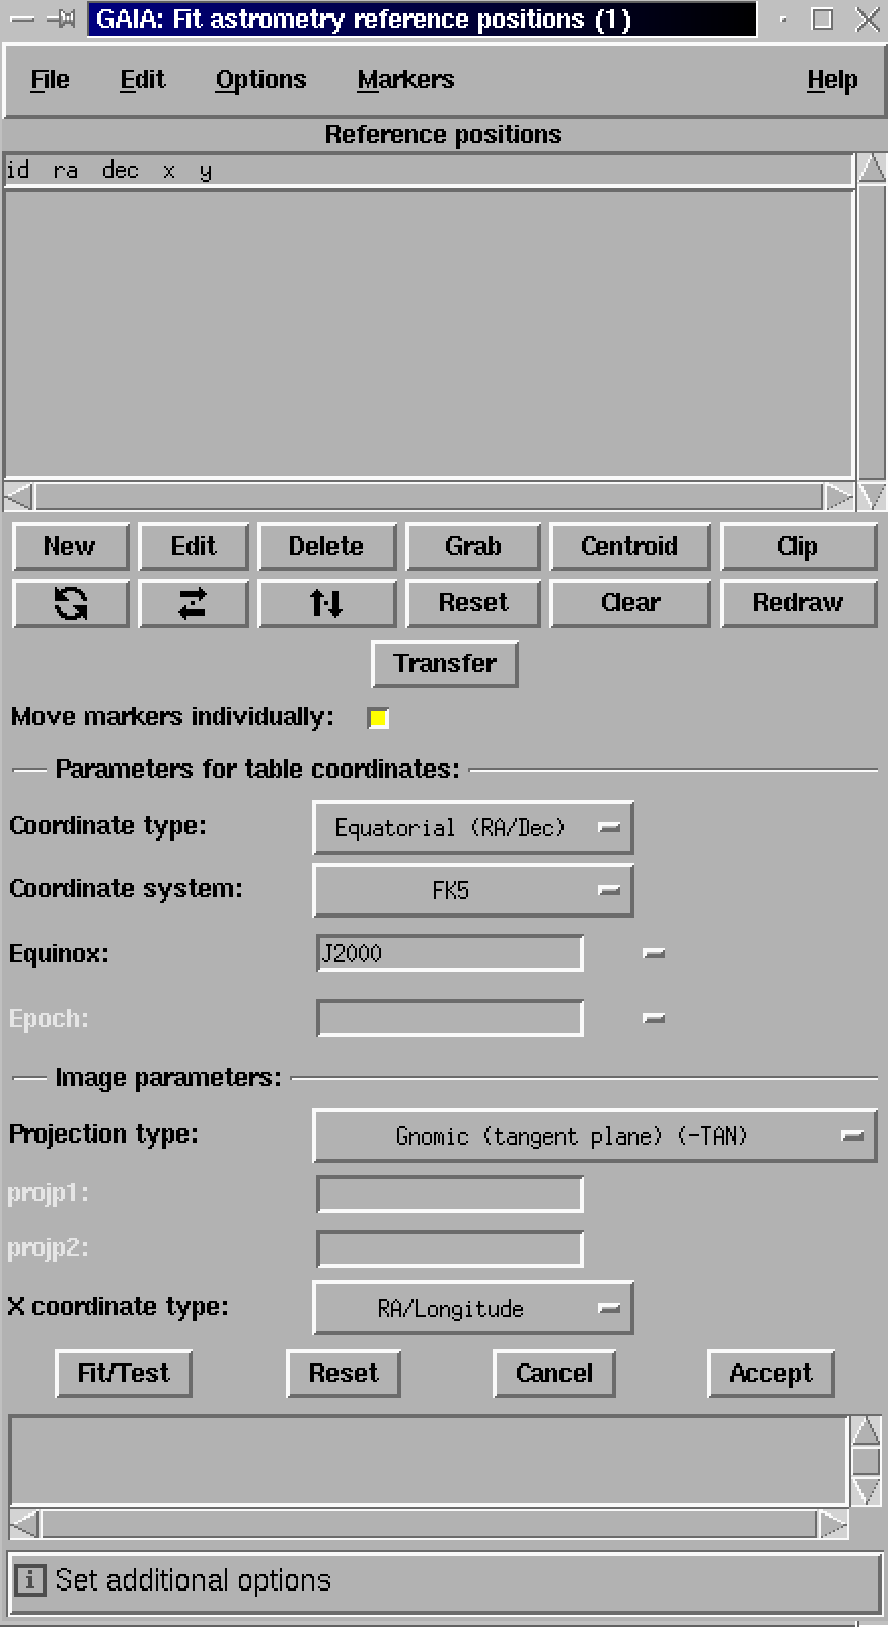
\includegraphics[clip,scale=0.5]{sun223_figures/gaia1}
  \caption{The main GAIA dialogue box used to create an RA/DEC calibration.}
  \label{fig:gaia1}
  \end{center}
  \end{figure}

\item Indicate the co-ordinate system in which your feature positions are
expressed. Do this by specifying suitable values using the \emph{co-ordinate
system:}, \emph{Equinox:} and \emph{Epoch:} buttons. You will usually have
either (FK4, equinox B1950) or (FK5, equinox J2000) positions. The epoch
defaults to B1950 for FK4 positions, and J2000 for FK5 positions.

\item Press the \emph{New} button, to indicate that you want to add some
new positions to the (currently empty) list of reference positions. This
should produce the dialogue box shown in
Figure~\ref{fig:gaia2}.

  \begin{figure}[htb]
  \begin{center}
  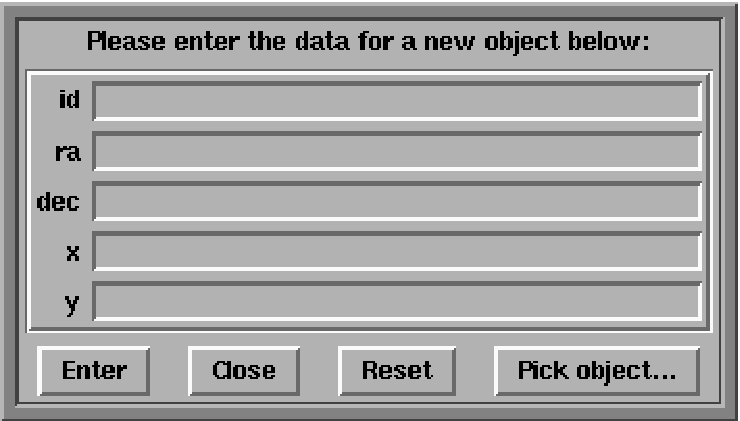
\includegraphics[clip,scale=0.5]{sun223_figures/gaia2}
  \caption{The GAIA dialogue box used to give a new reference position.}
  \label{fig:gaia2}
  \end{center}
  \end{figure}

\item Now press the \emph{Pick object...} button. This will create the
dialogue box shown in Figure~\ref{fig:gaia3}.
The upper black box displays a section of the main image centred on the position
of the cursor. Position the cursor in the main GAIA window over a feature
(usually a star) for which you know the RA/DEC. This star should appear
in the box in the ``object picker'' dialogue box (Figure~\ref{fig:gaia3}).
If there are any other significant features visible in the box, you should
reduce the size of the box using the zoom-out button below the displayed
image section. Once you are happy with the
sample size, re-position the cursor over the star and press the left
mouse button. The pixel co-ordinates at the centre of the feature are
displayed in the \emph{Image X:} and \emph{Image Y:} fields within the
object picker dialogue box

  \begin{figure}[htb]
  \begin{center}
  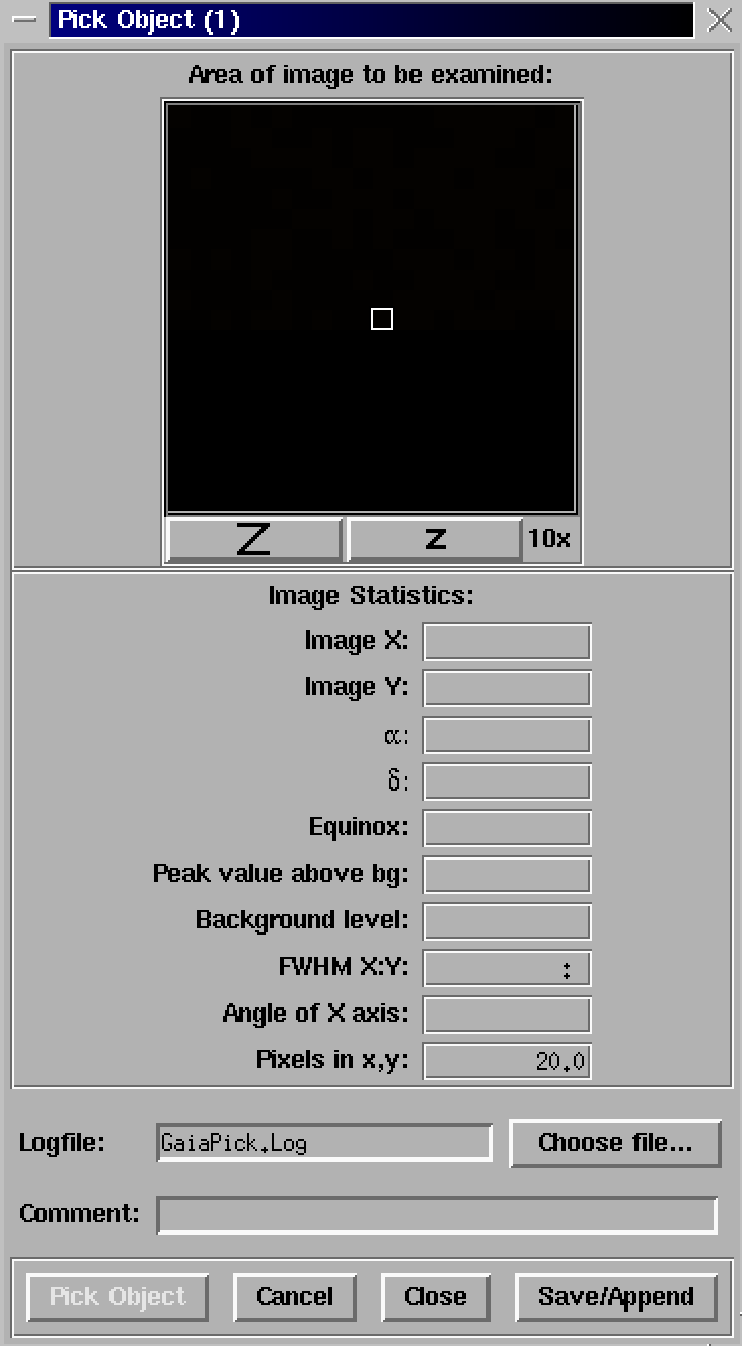
\includegraphics[clip,scale=0.5]{sun223_figures/gaia3}
  \caption{The GAIA object picker dialogue box.}
  \label{fig:gaia3}
  \end{center}
  \end{figure}

\item Raise the dialogue box shown in Figure~\ref{fig:gaia2}. You should
find that the pixel co-ordinates of the star have been copied into the
X and Y fields. Click in the \emph{ra} field, and enter the RA of the
star (\emph{e.g.} "12:23:34.1"). Then do the same with the \emph{dec} field. Then
click in the \emph{id} field, and enter an integer value which can be
used to identify the star (for instance, use 1 for your first star, 2 for
your second, \emph{etc}). The star is now fully specified, so press the
\emph{Enter} button. After confirmation, this will add the object into
the list of reference objects in the dialogue box shown in
Figure~\ref{fig:gaia1}.

\item All the windows will remain open, so you can continue to enter new
reference stars in the same way. First click on the \emph{Pick Object}
button in the dialogue box shown in Figure~\ref{fig:gaia3}. Then position
the cursor over a star in the main window, click with the left button, enter
the RA, DEC and ID values for the star, and press \emph{Enter}.

\item Once you have entered all your reference positions, close the
dialogue boxes shown in Figures~\ref{fig:gaia2} and~\ref{fig:gaia3} by
pressing the \emph{Close} button in each one.

\item Press the \emph{Fit/Test} button in the dialogue box shown in
Figure~\ref{fig:gaia1}. This will calculate the best RA/DEC calibration
given your reference positions. It then uses this calibration to work out
the pixel co-ordinates corresponding to each of your reference positions,
and displays markers in the main image at these pixel co-ordinates. You
should find that they fall on top of the corresponding stars. If they do
not, you have probably entered a bad RA or DEC value. You should correct
the reference positions, and then press the \emph{Fit/Test} button again. To
correct the reference positions, position the pointer over the erroneous
line in the list of reference positions, and click the left button (the
selected line will be highlighted). Then click the \emph{Edit} button, the
dialogue box shown in Figure~\ref{fig:gaia2} will re-appear, loaded with
the details of the selected feature. Correct the values, and then press
\emph{Enter}, followed by \emph{Close}. Now you can press \emph{Fit/Test}
again to re-calculate the RA/DEC calibration.

\item Once you are happy with the calibration, press the \emph{Accept}
button. You can now save the RA/DEC calibration by pressing the \emph{File}
menu button in the main window, and then the \emph{Save as} menu item. Use the
resulting dialog box to save the image (with the RA/DEC calibration) in a
new file. This is most simply done by entering the new file name in the
\emph{Selection} box, and pressing \emph{OK}. Do not worry if a message is
displayed saying that the WCS could only be saved as an AST native
representation.

\end{enumerate}

\newpage

\section{\label{APP:SNGBM}\xlabel{CalculationofStokesVectorsinSingle-beamMode}
Calculation of Stokes Vectors in Single-beam Mode}

This section describes the algorithm used by \htmlref{POLCAL}{POLCAL} to
created Stokes vectors from single-beam data. It assumes that the data is
single-waveband. Spectropolarimetry data is processed in the same way,
except that an intensity `image'' is actually an intensity ``cube''
containing two spatial axes and one spectral axis. In this context, no
distinction is usually made between spatial and spectral axes\footnote{
The only exception is that when data is ``smoothed'' it is only smoothed
in the two spatial axes - no smoothing occurs between spectral channels.}.

Given a set of observed intensity values and corresponding variance values,
a set of Stokes vectors with associated variances can be produced
following the technique described by Sparks \& Axon (\emph{P.A.S.P.} in
prep.). The full error analysis given by Sparks \& Axon also allows the
estimation of the co-variance between Q and U which occurs when
non-orthogonal analyser positions are used. POLCAL produces these
co-variances and stores them as a separate 2D NDF within the POLPACK
extension of the output cube. However, the calculation of the degree and
orientation of the polarization performed by \htmlref{POLVEC}{POLVEC} and
\htmlref{POLBIN}{POLBIN} do not as yet use these co-variances\footnote{Neither
do they use the improved de-biassing technique described by Sparks \&
Axon.}. It is hoped that this will be rectified in a future release of
POLPACK.

The technique described by Sparks \& Axon is basically a case of fitting
the intensity values at each pixel with the following function:

\begin{myquote}
\begin{eqnarray}
  \label{EQN:IEXP}
  I'_{k} & = & \frac{t}{2}( I + \epsilon.( Q.\cos 2\phi_{k} + U.\sin 2\phi_{k} ) )
\end{eqnarray}
\end{myquote}

where $I'_{k}$ is the expected intensity in image $k$, $t$ is the analyser
transmission factor, $\epsilon$ is the analyser efficiency factor, and
$\phi_{k}$ is the anti-clockwise angle from the reference direction to the
analyser position (or effective analyser position if using a half-wave
plate) for image $k$. The Stokes parameters $I$, $Q$ and $U$ are chosen
to minimize $\chi^2$, half the weighted sum of the squared residuals between
the expected intensity $I'_{k}$ and observed intensity $I_{k}$, where the sum is taken over all images
(\emph{i.e.} all values of $k$). The weights used are the reciprocals of
the variances associated with the observed intensity values:

\begin{myquote}
\begin{eqnarray}
  \label{EQN:CHI}
  \chi^2 & = & \frac{1}{2}\sum_{k} \frac{(I_{k}-I'_{k})^2}{\sigma^2_{k}}
\end{eqnarray}
\end{myquote}

A minimum of three images are required, taken at different analyser
positions, to perform this fit. The basic algorithm gives little
protection against badly aberrant input values (\emph{e.g.} cosmic rays,
etc.) which can corrupt the fit. However, if more than three images are
obtained with different half-wave plate positions, then an iterative
process can be used to identify and reject such aberrant data values.
This process works by first calculating the Stokes vectors using all
input data values. The expected intensity value at each input pixel is
then found from these Stokes vectors using equation \ref{EQN:IEXP}. The
residual between this expected intensity value and the observed intensity
value is then found. If this residual is larger than a specified
multiple\footnote{Specified by POLCAL parameter NSIGMA.} of the standard
deviation associated with the observed intensity value, $\sigma_k$, then
the observed intensity value is rejected. The Stokes vectors are
calculated again, excluding all the rejected intensity values. This
process is repeated a number of times, as specified by POLCAL parameters
MAXIT and TOLR. The number of pixels rejected in each image at each iteration can
be displayed by setting POLCAL parameter ILEVEL to 3. There is an option
to reject output pixels (\emph{i.e.} set them bad) if more than a given
fraction of the input intensity values are rejected as aberrant by the
above iterative procedure (see parameter MINFRAC).

If no usable variances are available for the observed data values, the
simplest option is to assume a constant value of $1.0$ for $\sigma_{k}$
(\emph{i.e.} give all input values equal weight). In this case no
variances for $I$, $Q$ and $U$ can be produced, and the iterative rejection
of input data described above cannot be performed. This option can be
used by setting POLCAL parameter WEIGHTS to 4.

In the absence of input variances, another option is to estimate these
variances by looking at the deviations of the observed intensity values
from the best fitting sine curve given by equation \ref{EQN:IEXP}. This
allows variances for the output Stokes vectors to be created, and also
allows the iterative rejection of bad data. This option can be used by
setting POLCAL parameter WEIGHTS to 3. The technique is described in the
following pseudo-code, and is illustrated diagrammatically in
Figure~\ref{fig:varest}:

\begin{terminalv}
1    Fill the variance image with the value 1.0
2    Calculate Stokes vectors
3    Set ITER = 0
4    While ( not converged and ITER < MAXIT ) do...
5       Reduce the noise in the Stokes vectors
6       Calculate expected intensity values implied by the smoothed
          I, Q and U values
7       Find the squared residuals between these intensity estimates
          and the observed intensity values
8       Find the mean squared residual at each pixel position
9       Smooth the image holding these mean squared residual values
10      Copy this smoothed image to the current variance image
11      Copy the input intensity values, excluding values for which
          the squared residual found above is too large
12      Calculate I, Q and U again using only the copied input values,
          and the current variance image
13      Set ITER = ITER + 1
14   End do
15   Reject any Stokes vectors corresponding to pixel with few good
       input intensity values.
\end{terminalv}

  \begin{figure}[htbp]
  \begin{center}
  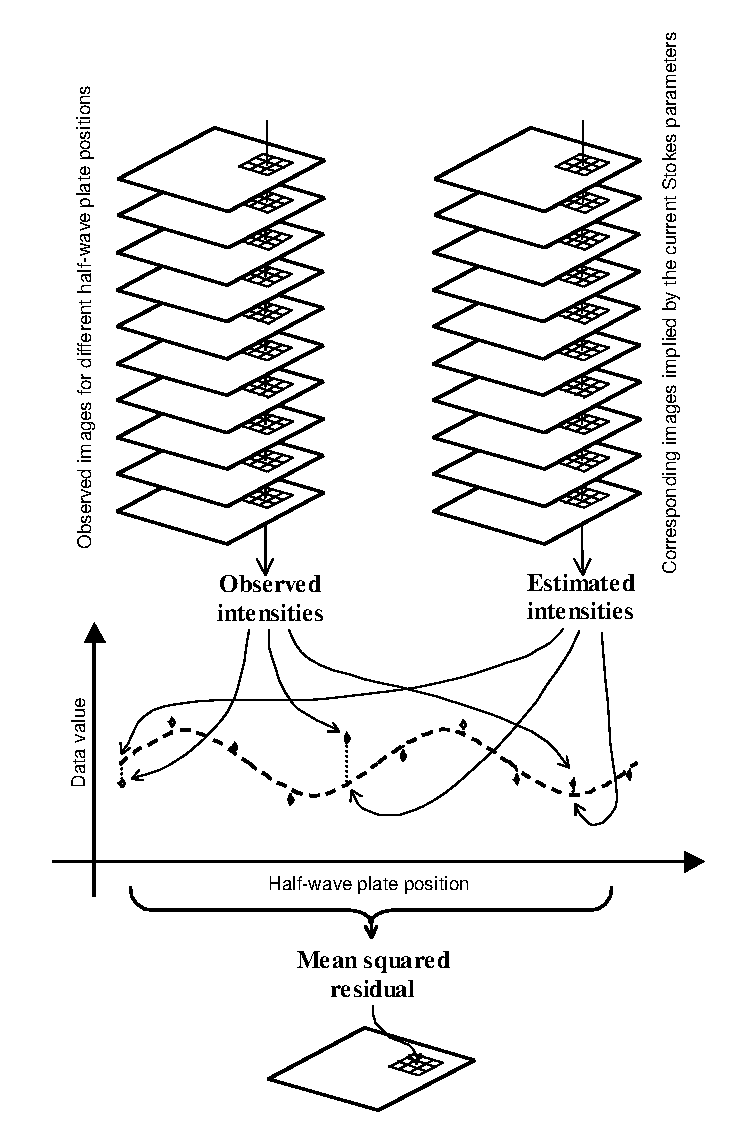
\includegraphics[clip,scale=0.9]{sun223_figures/varest}
  \caption[The estimation of input variances.]{The estimation of input variances. The observed and expected
           intensity images are combined to form a single variance image.}
  \label{fig:varest}
  \end{center}
  \end{figure}

Each step in this process is described further below:

\begin{enumerate}

\item The \emph{variance image} holds the variance to associate with each
input intensity value. Initially, all variances are set to $1.0$ so that
all input data values have equal weight. Note, there is only one variance
image. A given input pixel is given the same variance in equation
\ref{EQN:CHI}, no matter which input image it comes from. If this were
not the case (\emph{i.e.} if each input image had its own variance image)
the better images would receive higher weight, resulting in them being
fitted more closely. On the next iteration, they would then be found to
have smaller residuals, and so would receive even higher weight,
resulting in them being fitted even more closely. This circular process
would repeat until the fit was totally dominated by the best input image.

\item The Stokes vectors are calculated using the constant weights set up
in step 1. All input data is used.

\item The variable \verb+ITER+ counts the number of iterations which have
been performed.

\item Loop round performing iterations until the process converges, or
the maximum number of iterations specified by parameter MAXIT is reached.
If MAXIT is zero, the Stokes vectors produced in step 2 are returned.

The convergence criterion is specified by parameter TOLR. Convergence is
assumed to have been reached when the number of pixels rejected from each
input image changes by less than TOLR pixels between iterations. If the
number of pixels rejected from any image changes by more than the value
of TOLR, then another iteration is performed (subject to the MAXIT limit).
The default value for TOLR is zero, resulting in iterations being
performed until the number of pixels rejected from each image no longer
changes.

\item The three images holding $I$, $Q$ and $U$ are smoothed to reduce
the noise. The extent of the smoothing (in pixels) is controlled by POLCAL
parameter SMBOX. Setting SMBOX to 1 or 0 results in no smoothing
being performed.

As mentioned above, the likely error in a set of observed intensity
values can be estimated by comparing them with the best fitting sine
curve defined by the current Stokes vectors. This estimation can be
performed independently for each pixel. However, unless your images are
badly under-sampled, it is also reasonable in the absence of noise to
expect each image to be spatially smooth over some small scale. So we
could also estimate the noise by spatially smoothing each image and
looking at the residuals between the smoothed and original data. The two
methods can be combined by smoothing the Stokes vectors before finding the
estimated intensity values.

In some cases this smoothing is essential. For instance, consider the
case where only three analyser positions are available. In the absence of
any smoothing, the best fitting sine curve would always be an exact fit
to the three observed data values, no matter what the noise may be. Therefore
the input variances could not be estimated. Introducing some spatial
smoothing changes the expected intensity values so that they are no
longer identical to the observed values, thus producing non-zero
residuals and allowing the input variances to be estimated. In general,
the fewer the number of analyser positions, the more important is the
spatial smoothing.

However, spatial smoothing can introduce problems. The loss in resolution
can result in real structure being interpreted as noise (\emph{i.e.}
having large residuals). This in turn, can result in the input variances
being over-estimated, and pixels being rejected from the calculation of
the Stokes vectors. This is particularly apparent close to small bright
features such as stars, but generally affects any region with significant
spatial gradient. For this reason, you may want to consider turning off
the smoothing if you have sufficient analyser positions to manage without
it. Having said that, the smoothing is implemented in a way which
minimises these effects by minimising the loss of resolution. A common
method for smoothing an image is to convolve the image with some Point
Spread Function. For instance a block filter replaces each pixel with the
mean of the values within a box centred on the pixel. The smoothing
performed by POLCAL is not done in this way. Instead, a quadratic surface
is fitted to the data in the box, and the value of the fitted surface at
the central pixel is taken as the smoothed pixel value. This method is
illustrated in Figure~\ref{fig:quadfit}.

  \begin{figure}[htbp]
  \begin{center}
  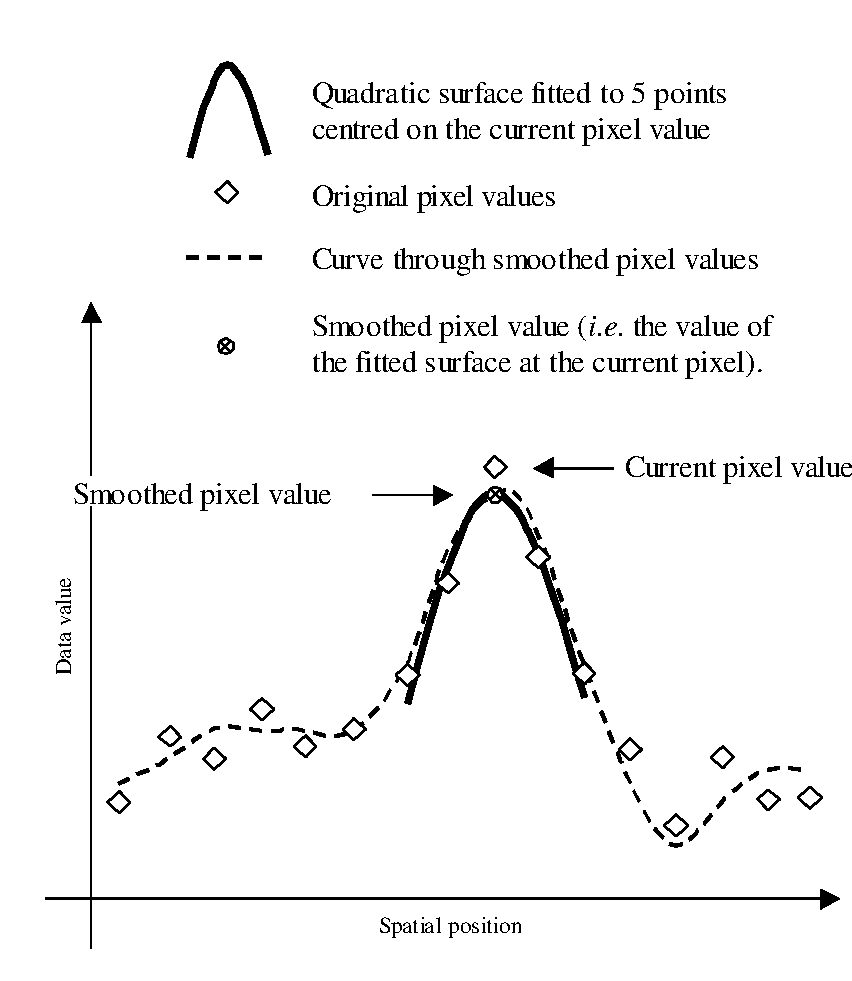
\includegraphics[clip,scale=0.75]{sun223_figures/quadfit}
  \caption[A 1-D representation of the smoothing performed in
  single-beam mode.]{A 1-dimensional representation of the smoothing performed by
           POLCAL in single-beam mode. In this example, each pixel is
           replaced by the value of a quadratic surface fitted to the
           nearest 5 data values.}
  \label{fig:quadfit}
  \end{center}
  \end{figure}

\item Equation \ref{EQN:IEXP} is used to calculate the intensity
values which would be expected on the basis of the smoothed Stokes vectors.

\item For each input image, the residuals between these expected intensity
values and the corresponding observed intensity values are found, and
squared. If the input images have differing zero points (caused by
instrumental effects or imperfect sky subtraction, for instance), then
the residuals for an individual image may well not have a mean of zero.
If left uncorrected, this would result in the mean squared residual at
each pixel being an over-estimate of the actual input variance. To reduce
this effect, there is an option (see parameter DEZERO) to apply a zero
point correction to each input image. This takes the form of a constant
value to be added to the image. This constant value is chosen so that the
mean of the residuals calculated in this step is zero, and is displayed
if parameter ILEVEL is set to 3 or more. If the DEZERO option is
selected, the zero point corrections are also used when calculating the
Stokes vectors themselves. The DEZERO option slows down the convergence
of the iterative procedure, resulting in a larger number of iterations
being required, and thus a larger run time.

\item The images containing the squared residuals are stacked together
into a single image holding the mean squared residual at each input pixel.

\item The image produced by the previous step is smoothed by replacing
each pixel with the mean of the values in a box centred on the pixel.
The size of the box used is the same as in step 5. So setting
parameter SMBOX to 1 or 0 will result in no smoothing being performed
at this point.

Consider again the case of three analyser positions. The residuals found in
step 7 will represent samples from the noise distribution. The
mean of the squared residuals in a small box thus gives an estimate of the
variance of the noise distribution. If the number of analyser positions,
$N$ is larger than 3, then the residuals produced in 7 will already
represent in some way the mean of $N$ noise samples, and so the need to
smooth the squared residuals is less.

\item These mean squared residuals are used as the variance estimates
for the next iteration. Note again, the same variance value is used for
a given pixel, no matter which input image the pixel comes from.

\item The residual between the observed and expected intensity values at
each pixel is compared with the square root of the current variance estimate
for the pixel. Any pixel for which the residual is greater than NSIGMA
times the standard deviation is flagged as bad, and is not used in the
next iteration.

\item A new set of Stokes vectors are produced using the observed
intensity values, and the current estimate of the variances. Any values
flagged as bad in the previous step are not included in the calculation.

\item Indicate that another iteration has been performed.

\item Go round for the next iteration.

\item Once convergence (or the maximum number of iterations) has been
reached, a check is made on the number of good intensity values which
contributed to each output Stokes vector. If too many of the input
intensity values were rejected as aberrant in step 11, then the Stokes
vector is set bad. This criterion is set by parameter MINFRAC, which
gives the minimum fraction of the input intensity values which must pass
the check in step 11 in order to create a good Stokes vector. The default
value of zero result in no Stokes vectors being rejected.

\end{enumerate}


\subsection{The Noise Level in Individual Input Images}
If the ILEVEL parameter is set to 3, the number of pixels rejected from
each input image at each iteration is displayed. In addition, the RMS
value of the residuals in each input image is displayed. This gives an
estimate of the mean noise level in each input image. Note, though, that
these RMS values are not used in the above algorithm, which gives equal
weight to all input images.

There is an option for POLCAL to store these mean variance values in the
VARIANCE components of the input images (see parameter SETVAR). If this
option is selected, the VARIANCE array in each input image is filled with
a constant value equal to the mean variance in the image estimated on the
final iteration.

So you may want to run POLCAL twice; the first time just to estimate the
mean noise level in each input image, and the second time to use these
mean noise levels to calculate the Stokes vectors. The first time you set
parameter WEIGHTS to 3 and SETVAR to TRUE, causing the input variances to
be estimated and stored in the input images. You then re-run POLCAL
setting parameter WEIGHTS to 1 in order to use these variances. This
would then produce Stokes vectors in which the better input images have
higher weight.

\subsection{Using POLSIM to Investigate Noise Characteristics}
The \htmlref{POLSIM}{POLSIM} application is a useful tool for
investigating the noise within a set of observed intensity images. It
takes in a cube of Stokes vectors as produced by \htmlref{POLCAL}{POLCAL},
together with a set of template intensity images, and creates a set of
intensity images analogous to the templates, but filled with the expected
intensity values given by equation \ref{EQN:IEXP}. The analyser properties
(angle, efficiency and transmission) are defined by the templates, as are
the required pixel positions.

So if you use POLCAL to generate a cube of Stokes vectors from a set of
observed intensity images, you could then use POLSIM to convert the
Stokes vectors back into intensity estimates, using the original observed
intensity images as templates. In a noise-free world, the resulting
estimated intensity images should be identical to the original observed
data. The presence of noise in the input data will result in this not
being the case, and the residuals between the two sets of images will
give an indication of the noise in the input images.

POLSIM can also be used to verify that the Stokes vectors produced by
POLCAL are consistent with the observed data.

\section{\label{APP:POLEXT}\xlabel{thepolpackndfextension}The POLPACK NDF Extension}

Figure~\ref{fig:polext} lists the items which may be stored in the
POLPACK extension within a data file. The \htmlref{POLEXP}{POLEXP} and
\htmlref{POLIMP}{POLIMP} applications may be used to transfer these items
to and from a set of corresponding FITS keywords. \htmlref{POLEXT}{POLEXT}
can be used to set them to explicit values (see \slhyperref{here}{section }
{}{SEC:IMPORT}). The contents of the POLPACK extension within an NDF may be
examined using POLEXT or the \xref{\texttt{hdstrace}}{sun102}{} command.

Versions of POLPACK prior to V2.0 included an extra item called ANGROT.
This gave the anti-clockwise angle from the first image axis to the
reference direction. POLPACK will still read these ANGROT values if they exist,
but will no longer write them. As of V2.0 the orientation of the reference
direction is specified instead by the POLANAL Frame added to the NDF WCS
component by POLIMP or POLEXT. If data written by POLPACK V2.0 or later
is read by an earlier version of POLPACK, a default value of zero will be
adopted for the missing ANGROT extension item (\emph{i.e.} it will be
assumed that the reference direction is parallel to the first image axis).

  \begin{figure}[htbp]
  \begin{center}
  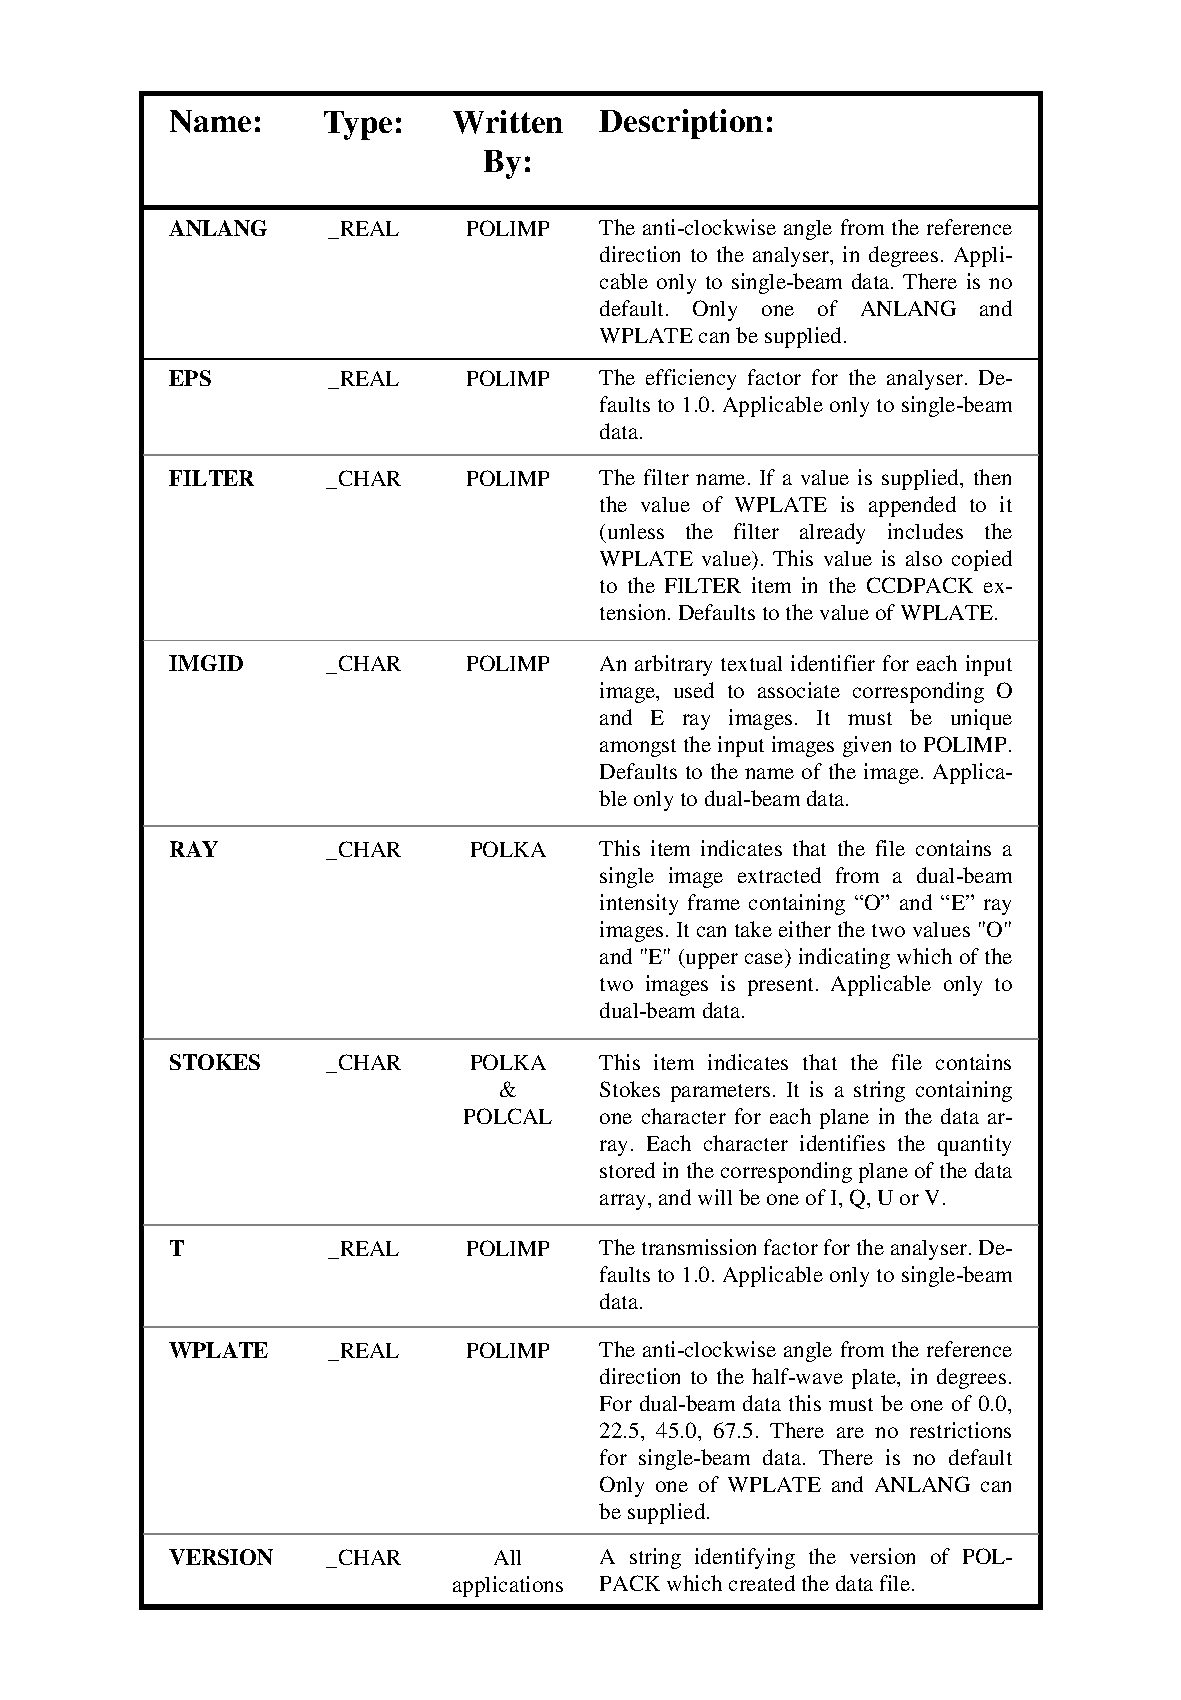
\includegraphics[clip,scale=0.75]{sun223_figures/polext}
  \caption{The allowed items within the POLPACK extension.}
  \label{fig:polext}
  \end{center}
  \end{figure}

\section{\label{APP:HISTORY}History}
This section describes the major changes introduced at each release of
POLPACK.



\subsection{V3.2-0}

\begin{itemize}
 \item A new command called POLROTREF has been added which will rotate
 the reference direction used by a pair of Q and U images.
 \item The POLVEC command now omits vectors from positions that have
 negative total intensity values.
\end{itemize}


\subsection{V3.1-5}

\begin{itemize}
 \item A bug in POLIMAGE that caused an error to be reported when deleting
 an AXIS Frame from the NDF WCS FrameSet has been fixed.

 \item POLVEC now uses the absloute value of I to normalise the other STokes
 vectors. Previously, a negative value of I would cause the normalised Q
 and U values to change sign, resulting in the vector rotating by 90
 degrees.
\end{itemize}


\subsection{V3.1-3}

\begin{itemize}
 \item Error messages indicating that a required column is not available
 have been expanded to suggest that deleting your \$HOME/.polpackrc
 file may solve the problem. This file can be left in a corrupt condition
 if a command fails whilst using the GAIA polarimetry toolbox.

\end{itemize}

\subsection{V3.1}

\begin{itemize}
\item POLPACK is now linked with native PGPLOT, instead of the Starlink
GKS-based version of PGPLOT.

\item The hidden command DATAPIC (used within POLKA) has been removed.

\end{itemize}

\subsection{V3.0}

\begin{itemize}
\item Most POLPACK commands have been changed to allow the processing of
spectropolarimery data. The main exception to this is the POLKA command,
which cannot be used with spectropolarimetry data. Instead, you should
align the data manually, and then use POLCAL directly to create Stokes
vectors.

\item Bugs have been fixed which allow catalogues in STL and TST formats
to be used (see \xref{SUN/190}{sun190}{FORMAT}).

\item A bug in POLPLOT has been fixed which caused inappropriate
text to be used for the default key heading.

\item A new hidden command POLZCONV has been added to transform between
calibrated values and pixel values along any spectral channel axis
present in a vector catalogue. This command is not intended for
interactive use.

\item Two new hidden commands POLWRTCL and POLRDCL have been added to
transfer catalogue data to and from the polarimetry toolbox within
\xref{GAIA}{sun214}{} (SUN/214). These commands are not
designed for interactive use.

\item POLIMP has a new parameter called ABORT which can be set TRUE
to force POLIMP to abort if any input data file cannot be processed.

\end{itemize}

\subsection{V2.1-7}
\begin{itemize}

\item A new logical-valued parameter called INTEGRATE has been added to
\htmlref{POLBIN}{POLBIN}. If set to a true value, the output catalogue
contains only a single vector formed by binning \emph{all} vectors
within the input catalogue. Otherwise, the output catalogue contains
vectors for a grid of bins determined by the BOX parameter, as before.

\item Two new hidden commands POLWRTCL and POLRDTCL have been added to
transfer catalogue data to and from the polarimetry toolbox within
\xref{GAIA}{sun214}{} (SUN/214). These commands are not
designed for interactive use.
\end{itemize}

\subsection{V2.1-5}

\begin{itemize}
\item The way \htmlref{POLBIN}{POLBIN} chooses the location of its bins
has been changed. The bins are now chosen so that origin of the (X,Y)
co-ordinate system (as defined by the X and Y columns in the input
catalogue), is always at the corner of a bin.

\item The WCS information stored with the output cube created by
\htmlref{POLCAL}{POLCAL} now has three axes instead of two (the Stokes
axis is now described in addition to the two spatial axes).

\item A new parameter called TRIMBAD has been added to \htmlref{POLCAL}{POLCAL}
to enable the output cube to be trimmed to exclude any borders of bad pixels.

\item \htmlref{POLBIN}{POLBIN} and \htmlref{POLVEC}{POLVEC} can now
optionally add RA and DEC columns to their output catalogues, so long as
suitable WCS information is available. See the new parameter RADEC.

\item The WCS FrameSet stored within catalogues by \htmlref{POLBIN}{POLBIN}
and \htmlref{POLVEC}{POLVEC} now include a GRID Frame describing the
grid co-ordinate system of the Stokes cube.

\item \htmlref{POLPLOT}{POLPLOT} now allows the key to be placed inside the
vector map by giving a negative value for the KEYPOS parameter. The text
included in the key can be specified using the Title attribute of
parameter KEYSTYLE.

\item The default vector scaling used by \htmlref{POLPLOT}{POLPLOT} has been
improved in cases where debiassing causes many zero length vectors to be
present.

\end{itemize}

\subsection{V2.0-14}

\begin{itemize}

\item A new command \htmlref{POLVERSION}{POLVERSION} has been added to check
the version number of the installed package.

\item The names of catalogues provided in response to parameter prompts
can now contain shell meta-characters (\emph{e.g.} \verb+$HOME/mycat+,
\verb+~/mycat+, \emph{etc.}).

\item The output cube created by POLCAL in dual-beam mode now covers the
union of the input frames, rather than the intersection.

\item A bug has been fixed which could cause the masks displayed by POLKA
in dual-beam mode to jump around as different images were selected.

\item A bug has been fixed in POLKA which caused the output NDFs to have
the wrong names if an image was supplied for parameter REFIN. The output
images corresponding to the first input image were stored in files
appropriate for the \emph{second} input image, \emph{etc.}, and the
output images for the final input image were not produced at all.

\item The use of the MARGIN parameter by POLPLOT to determine the width of
the margins to place around the annotated axes has been changed. The widths
of the margins used to be specified as fractions of the height or width
of the corresponding DATA plot. They are now given as fractions of the
height or width of the current picture.

\item The latex and hypertext documents now include the POLSTACK command,
previously only documented in the on-line help library.

\end{itemize}

\subsection{V2.0}

\begin{itemize}

\item \htmlref{POLCAL}{POLCAL} can now produce Stokes vectors from
single-beam data.

\item SUN/223 has been updated to include discussion of single-beam data.

\item \htmlref{POLKA}{POLKA} will now allow rotation between images in
single-beam mode.

\item POLPACK (including \htmlref{POLKA}{POLKA}) may now be used from the
ICL and IRAF cl command languages.

\item \htmlref{POLKA}{POLKA}) now has a REFIN parameter which may be used
to specify a reference image to which the other images should be aligned.
A reference image specified in this way will not be processed to create
any output files.

\item The NEWCOLMAP parameter has been removed from \htmlref{POLKA}{POLKA}.
POLKA will now use a private colour map automatically when necessary.

\item The Dump and Restore commands in the \htmlref{POLKA}{POLKA} File menu
now have an option to dump and restore the feature positions, masks and sky
areas for the display image alone to a text file.

\item A new command called \htmlref{POLSIM}{POLSIM} has been added, which
creates simulated intensity data from a cube of Stokes vectors and a set
of template intensity images. This is a useful tool for investigating
noise characteristics within a set of intensity images.

\item A new command called \htmlref{POLIMAGE}{POLIMAGE} has been added
which allows a 1 or 2 dimensional image to be created from a column of a
catalogue.

\item The reference direction for Stokes parameters created by
\htmlref{POLCAL}{POLCAL}, \htmlref{POLBIN}{POLBIN} and
\htmlref{POLVEC}{POLVEC} has been changed.
Prior to V2.0 the reference direction was the WPLATE=0 position (\emph{
i.e.} the direction of the fixed analyser). As of V2.0, the reference
direction will be north if there is WCS information available to define
north, or the positive Y axis (\emph{i.e.} the second pixel axis)
otherwise. \htmlref{POLVEC}{POLVEC} and \htmlref{POLBIN}{POLBIN} can still read data sets
created by earlier versions of POLPACK which use the previous convention, but will
write data sets using the new convention.

\item The angles produced by \htmlref{POLBIN}{POLBIN} and
\htmlref{POLVEC}{POLVEC} which
give the orientation of the polarization vectors are now referred to the
same reference direction as the Stokes parameters. Previously, these
angles were measured anti-clockwise form the positive X axis (\emph{
i.e.} the first pixel axis). They are now measured anti-clockwise from
the same reference direction as the Stokes parameters.
\htmlref{POLPLOT}{POLPLOT}
will automatically determine the correct convention to use, based on the
POLPACK version number stored in the supplied catalogue.

\item The way in which the reference direction is recorded within a
POLPACK data file has been changed. Prior to V2.0, the POLPACK extension
item named ANGROT was used. The reference direction is now specified by
the POLANAL co-ordinate Frame added to the WCS component when
\htmlref{POLIMP}{POLIMP} or \htmlref{POLEXT}{POLIMP} is run. V2.0 will read
ANGROT values in existing data sets, but will no longer write them.

\item The facilities for processing textual values within an import
control table used by \htmlref{POLIMP}{POLIMP} have been expanded.
Concatenation and replacement can now be combined together, using
parentheses to indicate the order in which sub-expressions should be
evaluated. References to keywords may be included in a replacement
specification (on either side of the equals sign) by enclosing the name
in parentheses. In fact such parentheses may include any general
character expression, containing nested replacement specifications,
concatentation, \emph{etc.}

\item The choice of default vector scale in \htmlref{POLPLOT}{POLPLOT}
has been improved. It now uses the 90\% percentile point, so that 10\% of
all vectors are at least equal to 1/15th of the length of the smaller plot
dimension.

\item The facilities for accessing groups of data files have been changed
to allow multiple NDFs within a single container file to be read.

\item A bug has been fixed which limited the number of data files which
could be processed by \htmlref{POLIMP}{POLIMP} when run as a monolith.

\item A bug in \htmlref{POLEXT}{POLEXT} has been fixed which prevented
POLEXT from being able to change an IMGID value.

\item Specifying the keyword STARTHELP when starting \htmlref{POLKA}{POLKA}
no longer requires POLKA to use a private colour map.

\item A bug in \htmlref{POLKA}{POLKA} has been fixed which resulted in a
Tcl error being reported when Saving or Exiting if any of the image names
begin with an upper case letter.

\item \htmlref{POLEXT}{POLEXT} and \htmlref{POLIMP}{POLIMP} no longer abort
if non-unique IMGID values are supplied. This allows IMGID values to be set
for  extracted O and E ray images.

\item \htmlref{POLEXT}{POLEXT} now allows POLPACK extension items to be
set for Stokes cubes and extracted O or E ray images, as well as raw
intensity images. The extension items are now written to output
parameters as well as to the screen.

\end{itemize}



\subsection{V1.1}
The handling of World Co-ordinate System (WCS) information within POLPACK
has been improved, and is now consistent with WCS handling within KAPPA
V0.13:

\begin{itemize}
\item New sections have been added to SUN/223 describing the use of
RA/DEC calibrations within POLPACK, and how to use GAIA to create them.
\item POLKA now propagates WCS information from input to output. This makes
it possible to retain WCS information throughout an entire POLPACK
reduction.
\item The COSYS parameter used by POLPLOT has been replaced by FRAME.
A new parameter called EPOCH has been added to allow the specification of
an epoch for celestial co-ordinate systems.
\item POLVEC no longer stores a GRID co-ordinate Frame in the output
catalogue (since there is no data grid defined within a catalogue).
\item WCS information can now be read from a FITS or IRAS90 NDF extension
if the NDF has no WCS component.
\item A bug has been fixed which caused POLPLOT to display vectors in
incorrect positions when annotating the axes with sky co-ordinates. This bug
was not seen if the vectors were plotted over an existing picture.
\item Catalogues created by POLVEC now inherit the Current co-ordinate Frame
from the supplied Stokes cube. Previously the Current Frame was always reset to
pixel co-ordinates.
\item The vector positions in the catalogue supplied to POLPLOT must now
be given in the Base Frame of the WCS information stored in the catalogue.
\end{itemize}

Other non-WCS related changes include:
\begin{itemize}
\item Vectors produced by POLPLOT no longer intersect the border.
\item If POLKA is used to define a sky region which is then transferred to
a second image, the sky region will be ignored if it does not have an overlap
with the second image. In this case, a warning is issued and the user is
asked to specify a new sky region for the second image.
\item The handling of graphical styles within POLPLOT (using parameters
STYLE and KEYSTYLE) is now consistent with KAPPA V0.13. In particular:
\begin{enumerate}
\item Defaults for unspecified plotting attributes are now read from file
\verb+$KAPPA_DIR/style.def+.
\item The values supplied for STYLE and KEYSTYLE are retained and re-used
on subsequent invocations of POLPLOT (unless new values are given).
\item The size of text produced for a given value of the Size attribute is
now (roughly) proportional to the size of the picture being used.
\item The default title is now obtained from the TITLE component of
the Stokes cube. Previously it was obtained from the Title attribute of
the WCS information.
\item A new parameter called ``RAY'' has been added to POLEXT to allow the RAY
component of the POLPACK extension to be assigned a value.
\end{enumerate}
\item The vertical spacing between lines in the key produced by POLPLOT can
now be controlled using the TextLabGap attribute (see parameter KEYSTYLE).
\item A new parameter called MARGIN has been added to POLPLOT. It can be
used to specify the widths of the margins left for axis annotation around
the vector map.
\end{itemize}

\begin{latexonly}

\cleardoublepage

\latexonlysection{Backpage alphabetic listing}

%
% set up a mini table of contents for the back pages of document.
%

\quickdes{POLBIN}{Bins a catalogue containing Stokes vectors.}{POLBIN}

\quickdes{POLCAL}{Calculates Stokes vectors from a set of aligned intensity images.}{POLCAL}

\quickdes{POLEXP}{Exports POLPACK information within an NDF to a FITS extension.}{POLEXP}

\quickdes{POLEXT}{Sets explicit values in the POLPACK extension.}{POLEXT}

\quickdes{POLIMP}{Imports POLPACK information into an NDF from a FITS extension.}{POLEXP}

\quickdes{POLHELP}{Displays textual help information for POLPACK.}{POLHELP}

\quickdes{POLIMAGE}{Converts a catalogue into an NDF.}{POLIMAGE}

\quickdes{POLKA}{An X-based GUI which converts raw photometric images into Stokes vectors.}{POLKA}

\quickdes{POLPLOT}{Displays polarization vectors supplied in a catalogue.}{POLPLOT}

\quickdes{POLROTREF}{Rotates the reference direction for a pair of Q and U images.}{POLROTREF}

\quickdes{POLSIM}{Produces intensity images corresponding to given Stokes vectors.}{POLSIM}

\quickdes{POLSTACK}{Stack a set of intensity images.}{POLSTACK}

\quickdes{POLVEC}{Converts a Stokes vector cube into a catalogue of polarization vectors.}{POLVEC}

\end{latexonly}

\end{document}
